%% lyan doctoral dissertation
%% init @ 03/26/2013
%% TODO: make a better template

%% the preamble below is from the template
%%
%% uctest.tex 11/3/94
%% Copyright (C) 1988-2004 Daniel Gildea, BBF, Ethan Munson.
%
% This work may be distributed and/or modified under the
% conditions of the LaTeX Project Public License, either version 1.3
% of this license or (at your option) any later version.
% The latest version of this license is in
%   http://www.latex-project.org/lppl.txt
% and version 1.3 or later is part of all distributions of LaTeX
% version 2003/12/01 or later.
%
% This work has the LPPL maintenance status "maintained".
% 
% The Current Maintainer of this work is Daniel Gildea.
%
% 2007/08/01
% LaTeX Package "ucr" is modified from LaTeX package "ucthesis."
% This modification is therefore under to the conditions of 
% the LaTeX Project Public License.
% Its formality is suitable for the dissertation of Universty of
% California, Riverside.
% This test document is for the convenience of all students of
% Universty of California, Riverside.
% Contact Charles Yang at chcyang@yahoo.com if you like.
% Charles Yang has nothing to do with the original author's sarcasm.
%
% \documentclass[11pt]{ucthesis}
% \documentclass[11pt]{ucr}
\documentclass[oneside,final]{ucr}
\usepackage{amssymb}
%%%%%%%%%%%%%%%%%%%%%%%%%%%%%%%%%%%%%%%%%%%%%%%%%%%%%%%%%%%%%%%%%%%%%%%%%%%%%%%%%%%%%%%%%%%%%%%%%%%%
\usepackage{bm}
\usepackage{amsmath}
%\usepackage[dvips]{graphicx}
%\usepackage{graphics}
\usepackage{graphicx}
\usepackage{caption,subcaption,enumerate}
\usepackage{flafter}
\usepackage{sw20uctd}

\usepackage{tikz}
\usetikzlibrary{shapes}
%% pseudocode related
\usepackage[nothing]{algorithm}
\usepackage{algorithmicx}
\usepackage[noend]{algpseudocode}
\usepackage{array}

\floatname{algorithm}{Pseudocode}
\renewcommand{\algorithmicrequire}{\textbf{Input:}}
\renewcommand{\algorithmicensure}{\textbf{Output:}}


\newtheorem{theorem}{Theorem}
\newtheorem{acknowledgement}[theorem]{Acknowledgement}
%%\newtheorem{algorithm}[theorem]{Algorithm}
\newtheorem{axiom}[theorem]{Axiom}
\newtheorem{case}[theorem]{Case}
\newtheorem{claim}[theorem]{Claim}
\newtheorem{conclusion}[theorem]{Conclusion}
\newtheorem{condition}[theorem]{Condition}
\newtheorem{conjecture}[theorem]{Conjecture}
\newtheorem{corollary}[theorem]{Corollary}
\newtheorem{observation}[theorem]{Observation}
\newtheorem{criterion}[theorem]{Criterion}
\newtheorem{definition}[theorem]{Definition}
\newtheorem{example}[theorem]{Example}
\newtheorem{exercise}[theorem]{Exercise}
\newtheorem{fact}[theorem]{Fact}
\newtheorem{lemma}[theorem]{Lemma}
\newtheorem{notation}[theorem]{Notation}
\newtheorem{problem}[theorem]{Problem}
\newtheorem{proposition}[theorem]{Proposition}
\newtheorem{remark}[theorem]{Remark}
\newtheorem{solution}[theorem]{Solution}
\newtheorem{summary}[theorem]{Summary}
\newenvironment{proof}[1][Proof]{\textbf{#1.} }{\ \rule{0.5em}{0.5em}}
\def\dsp{\def\baselinestretch{2.0}\large\normalsize}
\dsp

%% The user must use \textheight and \topmargin to control to button margin.
\textheight = 8.25in
\topmargin = 0.750in


%%%%%%%%%%%%%%%%%%%%%%%%%%%%%%%%%%%%%%%%%%%%%%%%%%%%%%%%%%

% non-math stuff

\newcommand{\myparagraph}[1]{{\smallskip\noindent{\bf #1}}}
\newcommand{\emparagraph}[1]{{\smallskip\noindent{\it #1}}}
\newcommand{\etal}{{\it et al.}}
\newcommand{\myif}{{\mbox{\rm\ if \ }}}
\newcommand{\mycase}[1]{\mbox{{\underline{Case #1}}:\/}}

\newcommand{\margincomment}[1]%
    {{%
      \marginpar{{\tiny\begin{minipage}{0.5in}
                       \begin{flushleft}
                          {#1}
                       \end{flushleft}
                       \end{minipage}
                }}
    }}


%%%%%%%%%%%%%%%%%%%%%%%%%%%%%%%%%%%%%%%%%%%%%%%%%%%%%%%%%%

% various letters

\newcommand{\hatc}{{\hat c}}
\newcommand{\hatC}{{\hat C}}
\newcommand{\hatr}{{\hat r}}
\newcommand{\hatx}{{\hat x}}
\newcommand{\haty}{{\hat y}}
\newcommand{\dotx}{{\dot x}}
\newcommand{\doty}{{\dot y}}
\newcommand{\dotr}{{\dot r}}
\newcommand{\boldx}{{\mathbf x}}

\newcommand{\doubledone}{{\bar 1}}
\newcommand{\doubledtwo}{{\bar 2}}
\newcommand{\barc}{{\bar c}}
\newcommand{\bart}{{\bar t}}

\newcommand{\barx}{{\bar x}}
\newcommand{\bary}{{\bar y}}
\newcommand{\barz}{{\bar z}}
\newcommand{\barr}{{\bar r}}
\newcommand{\barX}{{\bar X}}
\newcommand{\barY}{{\bar Y}}
\newcommand{\barZ}{{\bar Z}}
\newcommand{\bara}{{\bar a}}
\newcommand{\bard}{{\bar d}}
\newcommand{\barm}{{\bar m}}
\newcommand{\barA}{{\bar A}}
\newcommand{\barB}{{\bar B}}
\newcommand{\barC}{{\bar C}}
\newcommand{\barG}{{\bar G}}
\newcommand{\barE}{{\bar E}}
\newcommand{\barV}{{\bar V}}

\newcommand{\wbarC}{{\overline{C}}}
\newcommand{\wbarD}{{\overline{D}}}
\newcommand{\wbarN}{{\overline{N}}}
\newcommand{\wbarX}{{\overline{X}}}


\newcommand{\barbeta}{{\bar\beta}}
\newcommand{\bargamma}{{\bar\gamma}}
\newcommand{\apomega}{{\bar\omega}}

\newcommand{\bfr}{\boldsymbol{r}}
\newcommand{\bfv}{{\bf v}}
\newcommand{\bfx}{\boldsymbol{x}}
\newcommand{\bfy}{\boldsymbol{y}}
\newcommand{\bfz}{{\bf z}}
\newcommand{\bfQ}{{\bf Q}}
\newcommand{\bfR}{{\bf R}}
\newcommand{\bfS}{{\bf S}}
\newcommand{\bfT}{{\bf T}}
\newcommand{\bfV}{{\bf V}}
\newcommand{\bfone}{{\bf 1}}
\newcommand{\bfalpha}{\boldsymbol{\alpha}}
\newcommand{\bfbeta}{\boldsymbol{\beta}}

\newcommand{\calA}{{\cal A}}
\newcommand{\calB}{{\cal B}}
\newcommand{\calC}{{\cal C}}
\newcommand{\calD}{{\cal D}}
\newcommand{\calE}{{\cal E}}
\newcommand{\calG}{{\cal G}}
\newcommand{\calH}{{\cal H}}
\newcommand{\calJ}{{\cal J}}
\newcommand{\calK}{{\cal K}}
\newcommand{\calL}{{\cal L}}
\newcommand{\calM}{{\cal M}}
\newcommand{\calN}{{\cal N}}
\newcommand{\calS}{{\cal S}}
\newcommand{\calU}{{\cal U}}
\newcommand{\calX}{{\cal X}}
\newcommand{\calT}{{\cal T}}

\newcommand{\hatcalI}{{\hat{\cal I}}}
\newcommand{\barcalI}{{\bar{\cal I}}}
\newcommand{\dotcalI}{{\dot{\cal I}}}

\newcommand{\vecS}{{\bar S}}
\newcommand{\vecT}{{\bar T}}
\newcommand{\vecone}{{\bf 1}}
\newcommand{\tildec}{{\tilde c}}
\newcommand{\tilded}{{\tilde d}}
\newcommand{\tildeD}{{\tilde D}}
\newcommand{\tildeC}{{\widetilde C}}
\newcommand{\tildeZ}{{\tilde Z}}
\newcommand{\tilder}{{\widetilde r}}
\newcommand{\tildex}{{\widetilde x}}
\newcommand{\wtildeN}{{\widetilde N}}
\newcommand{\tildebfr}{\widetilde{\boldsymbol{r}}}
\newcommand{\tildebfx}{\widetilde{\boldsymbol{x}}}
\newcommand{\tildebfy}{\widetilde{\boldsymbol{y}}}

\newcommand{\barbfx}{\bar{\boldsymbol{x}}}
\newcommand{\barbfy}{\bar{\boldsymbol{y}}}
\newcommand{\hatbfx}{\hat{\boldsymbol{x}}}
\newcommand{\hatbfy}{\hat{\boldsymbol{y}}}
\newcommand{\dotbfx}{\dot{\boldsymbol{x}}}
\newcommand{\dotbfy}{\dot{\boldsymbol{y}}}

\newcommand{\wbarcalC}{{\overline{\calC}}}
\newcommand{\wbarcalD}{{\overline{\calD}}}
\newcommand{\eps}{{\epsilon}}

%%%%%%%%%%%%%%%%%%%%%%%%%%%%%%%%%%%%%%%%%%%%%%%%%%%%%%%%%%

\newcommand{\half}{{\mbox{$\frac{1}{2}$}}}
\newcommand{\threehalfs}{{\mbox{$\frac{3}{2}$}}}
\newcommand{\threefourths}{{\mbox{$\frac{3}{4}$}}}
\newcommand{\fivehalfs}{{\mbox{$\frac{5}{2}$}}}
\newcommand{\onethird}{{\mbox{$\frac{1}{3}$}}}
\newcommand{\twothirds}{{\mbox{$\frac{2}{3}$}}}
\newcommand{\fourthirds}{{\mbox{$\frac{4}{3}$}}}
\newcommand{\fivethirds}{{\mbox{$\frac{5}{3}$}}}
\newcommand{\fivefourths}{{\mbox{$\frac{5}{4}$}}}
\newcommand{\onefourth}{{\mbox{$\frac{1}{4}$}}}
\newcommand{\onefifth}{{\mbox{$\frac{1}{5}$}}}
\newcommand{\twofifths}{{\mbox{$\frac{2}{5}$}}}
\newcommand{\threefifths}{{\mbox{$\frac{3}{5}$}}}
\newcommand{\fourfifths}{{\mbox{$\frac{4}{5}$}}}
\newcommand{\ninefifths}{{\mbox{$\frac{9}{5}$}}}
\newcommand{\sevensixths}{{\mbox{$\frac{7}{6}$}}}
\newcommand{\oneeighth}{{\mbox{$\frac{1}{8}$}}}
\newcommand{\threeeighths}{{\mbox{$\frac{3}{8}$}}}
\newcommand{\fiveeighths}{{\mbox{$\frac{5}{8}$}}}
\newcommand{\seveneighths}{{\mbox{$\frac{7}{8}$}}}
\newcommand{\onetenth}{{\mbox{$\frac{1}{10}$}}}
\newcommand{\seventenths}{{\mbox{$\frac{7}{10}$}}}
\newcommand{\ninetenths}{{\mbox{$\frac{9}{10}$}}}
\newcommand{\twonineths}{{\mbox{$\frac{2}{9}$}}}
\newcommand{\fivenineths}{{\mbox{$\frac{5}{9}$}}}
\newcommand{\elevennineths}{{\mbox{$\frac{11}{9}$}}}
\newcommand{\threetwentieths}{{\mbox{$\frac{3}{20}$}}}
\newcommand{\twentyfivenineteenths}{{\mbox{$\frac{25}{19}$}}}

\newcommand{\sqrttwo}{\sqrt{2}}

%%%%%%%%%%%%%%%%%%%%%%%%%%%%%%%%%%%%%%%%%%%%%%%%%%%%%%%%%%

% various delimiters

\newcommand{\braced}[1]{{ \left\{ #1 \right\} }}
\newcommand{\angled}[1]{{ \left\langle #1 \right\rangle }}
\newcommand{\brackd}[1]{{ \left[ #1 \right] }}
\newcommand{\parend}[1]{{ \left( #1 \right) }}
\newcommand{\barred}[1]{{ \left| #1 \right| }}
\newcommand{\dbarred}[1]{{ \left\| #1 \right\| }}
\newcommand{\floor}[1]{{ \lfloor #1 \rfloor }}
\newcommand{\ceiling}[1]{{ \lceil #1 \rceil }}

%%%%%%%%%%%%%%%%%%%%%%%%%%%%%%%%%%%%%%%%%%%%%%%%%%%%%%%%%%

% some math symbols

\newcommand{\set}{\,{\leftarrow}\,}
\newcommand{\suchthat}{{\,:\,}}
\newcommand{\cost}{{\it cost}}
\newcommand{\yield}{{\it yield}}
\newcommand{\opt}{{\it opt}}

\newcommand{\algA}{{\bf A}}
\newcommand{\LHS}{{\rm LHS}}
\newcommand{\RHS}{{\rm RHS}}
\newcommand{\reals}{{\bf R}}
\newcommand{\posreals}{{\bf R}^+}

\newcommand{\assign}{{\,\leftarrow\,}}

\newcommand{\absvalue}[1]{{\barred{#1}}}
\newcommand{\posvalue}[1]{{\brackd{#1}^+}}

\newcommand{\NP}{{\mbox{\sf NP}}}
\newcommand{\PP}{{\mbox{\sf P}}}
\newcommand{\DTIME}{{\mbox{\sf DTIME}}}

\newcommand{\letbox}[1]{{\makebox[11pt]{{\small {$#1$}}}}}
\newcommand{\optstring}[1]{{ \frame{\;\raisebox{0pt}[12pt][5pt]{#1}\;} }}

\newcommand{\leftend}{{\diamond}}
\newcommand{\rightend}{{\diamond}}

%\newcommand{\argmin}{{\mbox{\rm argmin}}}
\DeclareMathOperator*{\argmin}{arg\,min}

\newcommand\litem[1]{\item{\bfseries #1\enspace}}
\newcommand{\ceil}[1] {\lceil #1 \rceil}
\newcommand{\naive}{na\"{\i}ve}
\newcommand{\LP}{\mbox{\rm LP}}
\newcommand{\OPT}{\mbox{\rm OPT}}
\newcommand{\ALG}{\mbox{\rm ALG}}
\newcommand{\LPR}[1]{{\mbox{\rm LPR#1}}}
\newcommand{\smallLPR}[1]{{\mbox{\tiny\rm LPR#1}}}
% algorithm names
\newcommand{\ESTA}{\mbox{\rm ESTA}} % 4approx
\newcommand{\EGUP}{\mbox{\rm EGUP}} % 3approx
\newcommand{\ECHS}{\mbox{\rm ECHS}} % 1.736
\newcommand{\EBGS}{\mbox{\rm EBGS}} % 1.575
\newcommand{\GUP}{\mbox{\rm GUP}}
\newcommand{\smallESTA}{\mbox{\tiny\rm ESTA}}
\newcommand{\smallEGUP}{\mbox{\tiny\rm EGUP}}
\newcommand{\smallECHS}{\mbox{\tiny\rm ECHS}}
\newcommand{\smallEBGS}{\mbox{\tiny\rm EBGS}}

\newcommand{\SOL}[1]{{{\mbox{\rm SOL}}_{#1}}}
\newcommand{\FTFP}{\mbox{\rm FTFP}}
\newcommand{\FTFL}{\mbox{\rm FTFL}}
\newcommand{\calI}{\mathcal{I}}
\newcommand{\avg}{{\mbox{\scriptsize\rm avg}}}

\newcommand{\dmax}{\text{dmax}}
\newcommand{\davg}{\text{davg}}
\newcommand{\favg}{f_{\text{avg}}}
\newcommand{\conn}{\text{conn}}
\newcommand{\cls}{\text{cls}}
\newcommand{\far}{\text{far}}

\newcommand{\sitesset}{\mathbb{F}}
\newcommand{\clientset}{\mathbb{C}}
\newcommand{\facilityset}{\overline{\sitesset}}
\newcommand{\demandset}{\overline{\clientset}}

%\newcommand{\dist}{{\mbox{dist}}}
\newcommand{\concost}{C^{\avg}}
\newcommand{\faccost}{F^{\avg}}
\newcommand{\tcc}{\textrm{tcc}}
\newcommand{\clsdist}{C_{\cls}^{\avg}}
\newcommand{\fardist}{C_{\far}^{\avg}}
\newcommand{\clsmax}{C_{\cls}^{\max}}
\newcommand{\clsnb}{N_{\cls}}
\newcommand{\farnb}{N_{\far}}
\newcommand{\wbarclsnb}{\wbarN_{\cls}}
\newcommand{\wbarfarnb}{\wbarN_{\far}}

\newcommand{\Exp}{\mbox{\rm Exp}}

\newcommand{\FacilityDistSort}{{\textsc{FacilityDistSort}}}
\newcommand{\NearestUnitChunk}{{\textsc{NearestUnitChunk}}}
\newcommand{\AugmentToUnit}{{\textsc{AugmentToUnit}}}
\newcommand{\connsum}{{\textrm{conn}}}

%%%%%%%%%%%%%%%%%%%%%%%%%%%%%%%%%%%%%%%%%%%%%%%%%%%%%%%%%%

% theorem and such

\newtheorem{fact}[theorem]{Fact}
\newtheorem{observation}[theorem]{Observation}

%%%%%%%%%%%%%%%%%%%%%%%%%%%%%%%%%%%%%%%%%%%%%%%%%%%%%%%%%%

\newcommand{\ignore}[1]{}

% for \cal definition
\makeatletter
\DeclareRobustCommand*\cal{\@fontswitch\relax\mathcal}
\makeatother
\setlength\headsep{-0.5in} 
\begin{document}

% Declarations for Front Matter

\title{Approximation Algorithms for the Fault-Tolerant Facility Placement Problem}
\author{Li Yan}
\degreemonth{June}
\degreeyear{2013}
\degree{Doctor of Philosophy}
\chair{Professor Marek Chrobak}
\othermembers{Professor Tao Jiang\\
Professor Stefano Lonardi\\
Professor Neal Young}
\numberofmembers{4}
\field{Computer Science}
\campus{Riverside}

\maketitle
\copyrightpage{}
\approvalpage{}

\degreesemester{Summer}

\begin{frontmatter}

\begin{acknowledgements}
  I would thank my advisor, Marek Chrobak, for bringing me
  into the PhD program of University of California
  Riverside, and for his guidance and patience on my study
  and research in the past five years. I am also grateful
  for the committee, Tao Jiang, Stefano Lonardi, and Neal
  Young for helpful discussions and comments on my research
  and this dissertation.

  The supportive environment of the algorithm lab and
  computer science department has made PhD study here a
  pleasant experience and I am grateful for Claire Huang,
  Wei Li and the algorithm lab for helpful discussions and
  stimulation of ideas.
\end{acknowledgements}

\begin{dedication}
\null\vfil
{\large
\begin{center}
  To my parents, who always have faith on my endeavor.
\end{center}}
\vfil\null
\end{dedication}

\begin{abstract}
  In this thesis we study the fault-tolerant facility
  placement problem (FTFP). In the FTFP problem, we are
  given a set of sites where we can open facilities, and a
  set of clients each with an integral demand. To satisfy
  their demands, clients need to be connected to open
  facilities in sites. The goal is to satisfy all clients'
  demands while minimizing the total cost, that is the cost
  of opening facilities and the cost of connecting clients
  to facilities. The problem is shown to be NP-hard and
  hence we study the approximation algorithms and their
  performance guarantee. Approximation algorithms are
  algorithms that run in polynomial time with provable
  performance when compared to optimal solutions.

  We present two techniques that lead to several LP-rounding
  algorithms with progressively improved approximation
  ratio. The best ratio we have is 1.575. We also study the
  primal-dual approaches. In particular, we show that a
  natural greedy algorithm analyzed using the dual-fitting
  technique gives an approximation ratio of O(logn). On the
  negative side, under a natural assumption, we give an
  example showing the dual-fitting analysis cannot give a
  ratio better than O(logn/loglogn).
\end{abstract}

\tableofcontents
\listoffigures
\listoftables

\end{frontmatter}

%% ch1 intro
\chapter{Introduction} \label{ch: intro}

\section{The Problem and the Background}
Facility location problems (FL) are about selecting a set of
candidate places to build (or open) facilities and
connecting clients to the facilities to satisfy their
demands. These problems model real world scenarios like
setting up warehouses to deliver commodities to retailers,
building power suppliers to serve the needs of a district of
residents, placing content servers in a network to send
files to subscribers. This simple model has been studied
extensively since 1960s (see books by Mirchandani and
Francis~\cite{Francis90}) due to its practical
significance. The problems have been an active topic in both
Operations Research and Computer Science research
communities, and a number of approaches have been proposed,
including heuristic solutions, branch and bound,
probabilistic methods, and approximation algorithms.

The facility location problems come with different
formulations and the variant studied in this thesis is
called the Fault-Tolerant Facility Placement problem
(\FTFP). In the {\FTFP} problem, we are given a set of sites
where one or more facilities could be opened, and a set of
clients each with a demand. A client needs to be connected
to several different facilities with the number of
connections equal to its demand. We are also given the
opening cost of a site, which is the cost to open one
facility at that site, and the distance between a site and a
client.  A solution consists of a specification of the
number of facilities to open at each site, and the number of
connections between a client and a site. Open multiple
facilities at the same site incurs a cost of the opening
cost for this site multiplied by the number of facilities
opened. The connection cost between a site and a client is
the number of connections times the distance between the
two, with the constaint that the number of connections
cannot exceed the number of open facilities at that
site. The FTFP problem asks for a solution with minimum
total cost, that is, the sum of facility cost and connection
cost.

As many optimization problems arising in practical
applications, the {\FTFP} problem is \NP-hard, and thus
precludes a promise for polynomial time algorithms that
solve the problems exactly. Nonetheless, there are
polynomial-time algorithms that deliver a solution with cost
only a small percentage off from the cost of optimal
solutions. These algorithms, known as approximation
algorithms and their performance analysis, are the subject
of this thesis.

By restricting the demand to $1$ for every client, we obtain
a more restricted problem, the uncapacitated facility
location problem (UFL). The {\UFL} problem has been studied
extensively in the past two decades. Many of our results on
{\FTFP} use the idea from the known results for {\UFL}. The
UFL problem with general distances has an algorithm with
approximation ratio $O(\log n)$ where $n$ is the number of
clients, due to Hochbaum~\cite{Hochbaum82}. A matching lower
bound of $\Omega(\log n)$ is immediate, as the UFL problem
contains the well-known Set Cover problem as a special
case. More on the relation of the two problems, UFL and Set
Cover can be found in Section~\ref{sec:hardness}.

Renewed interest in the UFL problem has been possible after
Shmoys, Tardos and Aardal~\cite{ShmoysTA97} showed that,
when distances form a metric, there is an algorithm with
$O(1)$ approximation ratio. Improved algorithms with more
sophisticated ideas have been proposed. The past two decades
has observed a sequence of improved approximation ratio,
from the original $4$-approximation of Shmoys
{\etal}~\cite{ShmoysTA97}, to the $1.488$-approximation by
Li~\cite{Li11}, the best known approximation ratio to date.

\section{Notation and Definition}
In the fault-tolerant facility placement problem ({\FTFP}),
we denote the set of sites as $\sitesset$ and the set of
clients as $\clientset$. Each client $j \in \clientset$ has
a demand $r_j$, meaning that client $j$ needs to be
connected to $r_j$ different facilities. The distance
between a site $i$ and a client $j$ is denoted as
$d_{ij}$. To open one facility at site $i$ incurs a cost of
$f_i$. To make one connection from client $j$ to a facility
at site $i$ incurs a cost of $d_{ij}$.  An {\FTFP} instance
is then fully specified by $\sitesset$, $\clientset$, $r_j$
for every $j\in\clientset$, and $d_{ij}$ for every
$i\in\sitesset,j\in\clientset$.

A solution to the {\FTFP} problem is a vector of $(\bfx,
\bfy)$ such that $x_{ij} \in \{0, 1, 2, \ldots\}$ denotes
the number of connections between site $i$ and client $j$,
and $y_i \in \{0, 1, 2\ldots\}$ denotes the number of
facilities opened at site $i$.  A feasible solution is one
such that $y_i \geq x_{ij}$ for every $i \in \sitesset, j
\in \clientset$ and $\sum_{i\in\sitesset} x_{ij} = r_j$ for
all clients $j \in \clientset$. We would like to have a
feasible solution with minimum total cost, that is $\sum_{i
  \in \sitesset} f_i y_i + \sum_{i \in \sitesset, j \in
  \clientset} d_{ij} x_{ij}$. For a given solution
$(\bfx,\bfy)$, we call the first term $\sum_{i \in
  \sitesset} f_i y_i$ the facility cost of the solution, and
the second term $\sum_{i \in \sitesset, j \in \clientset}
d_{ij} x_{ij}$ the connection cost of the solution.

For both the uncapacitated facility location problem (UFL)
and the fault-tolerant facility placement problem (FTFP), we
have a metric version of the problem in which the distances
satisfy the triangle inequality, that is, for any two
facilities/sites $i_1,i_2$ and any two clients $j_1,j_2$, we
have
\begin{equation*}
  d_{i_1 j_2} \leq d_{i_1 j_1} + d_{i_2 j_1} + d_{i_2 j_2}.
\end{equation*}
Unless otherwise stated explicitly, we assume the problem
under study is the metric version.

\section{Optimization Problem, P vs NP, and Approximation}
All problems studied in this thesis are optimization
problems. An optimization problem is defined by a set of
parameters and constraints and is either a minimization
problem or a maximization problem. Specifying the values of
the parameters defines an instance of the problem. A
feasible solution to an optimalization problem is a solution
that satisfies all the constraints. The problem also
specifies a cost function that evalutes every feasible
solution to a numerical cost. For a minimization problem, an
optimal solution is a feasible solution whose cost is no
more than the cost of any other feasible solution.

An algorithm is said to solve an optimization problem
exactly if for every instance, the algorithm always computes
an optimal solution, or reports that no feasible solution
exists. For problems that are \NP-hard, such an exact
algorithm that also runs in polynomial time is not possible
unless $\PP = \NP$. Therefore we focus our attention on
polynomial-time algorithms that computes a feasible solution
whose cost can be proved to be within some factor away from
an optimal solution's cost. Such algorithms are called
approximation algorithms.

\section{Hardness Results on Approximating UFL and FTFP}
\label{sec:hardness}

Not only is the FTFP problem \NP-hard, more can be said
about to what extent we can approximate an optimal
solution. Results showing that problems cannot be
approximated to certain numbers, using well repsected
assumptions like $\PP\neq \NP$, are called hardness results
and we present the hardness results on the {\FTFP} problem
in this section.

Since the fault-tolerant facility location problem (\FTFP)
contains the uncapacitated facility location problem (\UFL)
as a special case (setting all $r_j=1$ in {\FTFP} we get
{\UFL}) , any hardness result obtained on UFL remains
applicable to FTFP. In the following, we review some
well-known hardness results on UFL, with the implication
that the same claims hold for FTFP as well.

The UFL problem is easily seen to be NP-hard, as they
contain the Set Cover problem as a special case. The Set
Cover problem is that, given a universe $\,\calU = \{e_1,
\ldots, e_n\}$ and a collection $\calS$ of sets such that
$\calS = \{S_1, \ldots, S_m\}$ and $S_l \subseteq \calU$ for
$l=1,\ldots,m$, find a minimum number of sets in $\calS$ to
cover all elements in $\calU$. That is, find a set $\calS'
\subseteq \calS$ such that $\bigcup_{S\in \calS'} = \calU$
and $|\calS'|$ is minimized. It is well-known that the
Set Cover problem is NP-hard.

%%% NP-optimization problems:
%%% - can verify instance validity in polynomial time
%%% - can verify solution feasibility in polynomial time
%%% - can compute solution cost in polynomial time
%%%
%%% Turing reduction (polynomial time, then Cook reduction)
%%% from problem A to problem B
%%% given an algorithm for B, then can solve A by constructing
%%% an oracle machine with oracle for B.
\begin{proposition}\label{prop:UFLNP}
  The general~\footnote{\emph{general} means no restriction
    on the distances $d_{ij}$. This is in constrast with the
    \emph{metric} version where $d_{ij}$ satisfies the
    triangle inequality.} UFL problem is NP-hard.
\end{proposition}
\begin{proof}
  Reduction from the Set Cover problem. In the Set Cover
  problem, we are given a universe of elements, that is
  $\calU = \{e_1, \ldots, e_n\}$, and a collection of sets
  $\calS = \{S_1, \ldots, S_m\}$ such that $S_i \subseteq
  \calU$ for $i=1,\ldots,m$. We construct a general UFL
  instance like this: for each element $e_j, j=1,\ldots,n$,
  we have a client $j$; and for each set $S_i,
  i=1,\ldots,m$, we have a facility $i$. The facility cost
  $f_i=1$ for every facility
  $i=1,\ldots,m$~\footnote{Actually any value of $f_i > 0$
    will work, for example, we can set $f_i=100$ for every
    facility $i$.}. The distance $d_{ij} = 1$ if $e_j \in
  S_i$ and $d_{ij} = \infty$ if $e_j \notin S_i$. Clearly an
  optimal solution for the UFL instance can only use edges
  with $d_{ij} = 1$. It is easy to see that given any
  optimal solution to the Set Cover instance, we can
  construct an optimal solution for the UFL instance, simply
  by taking the facilities whose corresponding sets are
  chosen in the set cover. On the other hand, given an
  optimal solution to the UFL instance, we can only have
  $d_{ij}=1$ connections. This implies that, for every
  client $j$, the corresponding element $e_j$ is covered by
  some set $S_i$, whose corresponding facility $i$ is chosen
  to open in the {\UFL} solution. Let $I$ be the set of
  facilities chosen in the {\UFL} solution, it is easily
  seen that the corresponding sets in the Set Cover instance
  form a set cover.
\end{proof}

\begin{proposition} \label{prop:metricNP}
  The metric UFL problem is NP-hard.
\end{proposition}
\begin{proof}
  The reduction is also from the Set Cover problem. Unlike
  the general UFL problem, we can no longer have edges with
  length $1$ and $\infty$ now, as the distances are
  constrained by the triangle inequality. We still have sets
  $S_i$ in the Set Cover instance correspond to the
  facilities $i$ in the metric UFL instance, and elements
  $e_j$ in the Set Cover instance correspond to the clients
  $j$ in the metric UFL instance. Our facility cost $f_i =
  \epsilon$ for some small number $\epsilon > 0$, and every
  facility $i$ has the same facility cost. Our distance
  $d_{ij}$ is now $1$ if $e_j \in S_i$ and $3$ if $e_j
  \notin S_i$.

  Given the construction, it is clear that any optimal
  solution for the metric UFL instance cannot use an edge of
  distance $3$, as there exists another solution that beats
  such a solution with lower cost, namely a solution that
  opens all facilities with total cost $m\epsilon + n\cdot 1
  = m\epsilon + n$, as we can choose $\epsilon = 1/m^2$. It
  follows that any optimal solution for the metric UFL
  instance must have all clients connected at distance of
  $1$. Such a solution would have a facility set corresponds
  to a set cover for the Set Cover instance, as for every
  client $j$, the corresponding element $e_j$ is covered by
  some set $S_i$ corresponding to facility $i$, since
  $d_{ij} = 1$ implies $e_j \in S_i$.
\end{proof}

%%% MaxSNP, a technically difficult class of problems
%%% includes: Max2SAT, B-Max3SAT, B-VertexCover, B-IndependentSet, MaxCut
%%% Assume P != NP, MaxSNP hard problems cannot have PTAS.
Now we show the {\MaxSNP}-hardness of the metric UFL
problem. This implies that there exists some constant $c$
such that the metric UFL problem cannot be approximated to
better than $c$-approximation. As a consequence, the metric
UFL problem cannot have polynomial-time approximation scheme
(PTAS), that is, algorithms that for any constant $\epsilon
> 0$, compute a solution with cost no more than
$(1+\epsilon)$ from the optimal, and the running time is
polynomial in the input size with $\epsilon$ treated as a
constant.

\begin{proposition}\label{prop:maxsnp} \cite{GuhaK98}
  The metric UFL problem is {\MaxSNP}-hard.
\end{proposition}
\begin{proof}
  Sketch: The full proof can be found in~\cite{GuhaK98} and
  we only sketch the main idea here.

  The proof is by a reduction from the B-Vertex Cover
  problem, a problem known to be {\MaxSNP}-hard. In the
  B-Vertex Cover problem, we are given a graph $G=(V,E)$,
  and a constant $B$, such that every vertex $u\in V$ has
  degree no more than $B$. And the problem asks for a vertex
  cover with minimum size. That is, we are to find a minimum
  set $V' \subseteq V$ such that every edge $e \in E$ has at
  least one endpoint in $V'$.

  The idea is to show that, for any given constant $0 <
  \epsilon < 1$, given an algorithm for the metric UFL
  problem with approximation ratio $1+\epsilon$, we are able
  to find an algorithm for the B-Vertex Cover problem with
  approximation ratio $1+\epsilon'$ such that $\epsilon'$ is
  a constant depending on $\epsilon$ and possibly $B$, and
  $\epsilon'$ approaches $0$ as $\epsilon$ approaches
  $0$. It turns out that we can set $\epsilon' =
  (1+B)\epsilon$ for our purpose.

  Given an instance of B-Vertex Cover, we construct an
  instance of metric UFL. For every vertex $u \in V$ we have
  a facility $i$ and for every edge $e \in E$ we have a city
  $j$. $d_{ij} = 1$ if the corresponding edge $e$ of client
  $j$ is incident on vertex $u$, which corresponds to the
  facility $i$, $d_{ij} = 3$ otherwise. We set all
  facilities to have the same facility opening cost $f$,
  that is $f_i = f$ for all facilities $i$. The value of $f$
  is chosen to expedite the derivation of desired
  inequalities. We also assume that we know the size of an
  optimal vertex cover, call it $k$, as our choice of $f$
  depends on $k$. In general we do not know $k$, as it is
  {\NP}-hard to compute $k$, the optimal solution value for
  B-Vertex Cover. However, we can still proceed assuming
  knowing $k$, because we can perform the proof for every
  possible $k=1,2,\ldots,n$. If our proof goes through for
  every choice of $k$, our claim must hold on the (unknown)
  value of $k$ as well. The same trick is used in the proof
  of Theorem~\ref{thm:1463}.

  The proof completes by showing that we can use an
  $(1+\epsilon)$-approximation algorithm $\calA_{\smallUFL}$
  for metric UFL to construct an
  $(1+\epsilon')$-approximation algorithm
  $\calA_{\smallBVC}$ for B-Vertex Cover. Since B-Vertex
  Cover is \MaxSNP-hard, and therefore no such algorithm
  $\calA_{\smallBVC}$ exists unless $\PP=\NP$, we conclude
  that no such $\calA_{\smallUFL}$ can exist under the same
  assumption. Therefore the metric {\UFL} problem is
  \MaxSNP-hard as well.
\end{proof}

After we have shown the metric UFL problem is {\MaxSNP}-hard,
we focus on the metric version from now on. In the follow,
we mention UFL and FTFP without explicitly specifying that
their distances form a metric, that is, $d_{ij}$'s are
symmetric and satisfy the triangle inequality.

From Proposition~\ref{prop:maxsnp} we know there exists a
constant $c$ such that the {\UFL} problem cannot be
approximated better than $c$. The last piece of hardness
result presented in this section gives the best known such
constant $c=1.463$. This result is also due to Guha and
Khuller.
\begin{theorem}\label{thm:1463} \cite{GuhaK98}
  {\UFL} cannot be approximated to less than $1.463$ unless
  \\ 
  $\NP \subseteq \DTIME(n^{O(\log\log n)})$.
\end{theorem}
\begin{proof}
  The proof is by contradiction. More precisely, we show
  that if the metric UFL problem can be solved by a
  polynomial-time algorithm with approximation ratio
  $\gamma$ that is less than $\gamma_0 =
  1.463$~\footnote{$\gamma_0$ is the solution to the
    equation $\gamma = 1 + 2/e^\gamma$.}, then we would have
  a polynomial-time algorithm with approximation ratio
  $(1/\rho) \ln n$ for some constant $\rho > 1$ for the Set
  Cover problem. Here $n$ is the number of elements in the
  universe in the Set Cover instance. Using a result by
  Feige~\cite{Feige98}, the existence of a $(1/\rho) \ln n$
  approximation algorithm for a constant $\rho > 1$ implies
  $\NP \subseteq \DTIME(n^{O(\log\log n)})$.

  Given a Set Cover instance with a universe $\,\calU =
  \{e_j \suchthat j=1,\ldots, n\}$ of elements and a family
  of sets $\calS = \{S_i\suchthat i=1,\ldots,m\}$ with every
  set $S_i \in \calS$ being a subset of $\,\calU$. The proof
  proceeds in iterations. In each iteration we construct a
  metric UFL instance and run the supposedly
  $\gamma$-approximation algorithm for {\UFL}. After that we
  remove clients connected at distance of $1$ (call them
  \emph{covered} in this iteration) in the {\UFL}
  solution. So future iterations will deal with a smaller
  set of clients. We repeat until all clients are covered.

  Consider the $t^{th}$ iteration and let $n_t$ be the
  number of clients not yet covered. The metric {\UFL}
  instance for this iteration consists of a set of
  facilities $\sitesset$ corresponding to the set $\calS$,
  and a set of clients with one client $j$ for each
  uncovered element $e_j$. The distance $d_{ij}$ is $1$ if
  $e_j \in S_i$, and $3$ otherwise. The opening cost of all
  facilities are equal and we set every $f_i = c\,n_t / k$,
  where $c$ is some constant decided later to optimize our
  lower bound on approximation ratio. Here $k$ is the number
  of sets in an optimal solution for the Set Cover instance.
  Note that we can perform the rest of the proof for every
  possible $k=1,\ldots,n$, so we can assume we know $k$.

  Our construction ensures that, at any iteration, if the
  UFL solution found by the $\gamma$-approximation {\UFL}
  algorithm does not cover a large portion of the clients,
  then the ratio $\gamma$ between this UFL solution's cost
  and the optimal solution's cost must be at least
  $1.463$. The solution with $k$ facilities and all clients
  connected at distance $1$ is used for estimating the
  optimal solution's cost. The other case is that in every
  iteration we have an UFL solution that covers a large
  portion of clients. This would then give us a solution for
  the given Set Cover instance with cost (number of sets) no
  more than $(k/\rho) \ln n$, that is no more than $(1/\rho)
  \ln n$ times of an optimal solution for constant $\rho >
  1$. This then implies $\NP \subseteq \DTIME(n^{O(\log\log
    n)})$ by Feige's result~\cite{Feige98}.
%%  Let $k$ be the number of sets in an optimal solution for
%%  the Set Cover instance. Note that we can run the following
%%  for every $k=1,\ldots,n$, so we can assume we know $k$.  We
%%  now give the construction of the UFL instance. In
%%  iteration $t$, suppose we begin with $n_t$ elements
%%  uncovered. Then we have a UFL instance with $|\sitesset| =
%%  m, |\clientset| = n_t$, $d_{ij} = 1 \text{ or } 3$ and
%%  $f_i$ to be specified but all $i\in\sitesset$ have equal
%%  $f_i$, although $f_i$ is set to a different value in each
%%  iteration. Now suppose the UFL algorithm chooses $\beta_t
%%  k$ facilities and covers $\gamma_t n_t$ clients, the rest
%%  $(1-\gamma_t) n_t$ clients are then servied at a distance
%%  of $3$. The cost of this UFL solution is
%%\begin{equation*}
%%  \ALG_{\smallUFL} = \beta_t k f_i + \gamma_t n_t \cdot 1 + (1 -
%%  \gamma_t) n_t \cdot 3.
%%\end{equation*}
%%We set $f_i = c\,n_t / k$ for some constant $c$. Notice that
%%the same constant $c$ is used for all iterations and we
%%shall use $c$ to optimize our analysis on the lower bound of
%%approximation ratio of any UFL algorithms. The cost of the
%%UFL solution now becomes
%%\begin{equation*}
%%  \beta_t c n_t + \gamma_t n_t + 3 (1-\gamma_t) n_t = n_t
%%  (c\beta_t + 3 - 2\gamma_t).
%%\end{equation*}
%%
%%On the other hand, we know that there exists a solution with
%%$k$ facilities that covers all clients at distance $1$,
%%which corresponds to an optimal Set Cover solution. So an
%%optimal UFL solution has cost no more than
%%\begin{equation*}
%%  \OPT_{\smallUFL} \leq k f_i + n_t = c n_t + n_t = (1+c)n_t.
%%\end{equation*}
%%
%%Since we are running an $\alpha$-approximation algorithm for
%%the UFL instance, we have
%%\begin{equation*}
%%  \alpha \geq \frac{\ALG_{\smallUFL}}{\OPT_{\smallUFL}} \geq \frac{n_t
%%  (c\beta_t + 3 - 2\gamma_t)}{(1+c)n_t} = \frac{\beta_t + 3 -
%%2\gamma_t}{1+c}.
%%\end{equation*}
%%
%%Let $\rho > 1$ be some fixed constant. Now we have two
%%cases:
%%
%%\mycase{1} There exists some iteration $t$ such that $\gamma_t <
%%1 - e^{-\rho\beta_t}$. Then we have
%%\begin{equation*}
%%  \alpha > \frac{c\beta_t + 3 - 2 (1 - e^{-\rho\beta_t})}{1+c} =
%%  \frac{c\beta_t + 1 + 2 e^{-\rho\beta_t}}{1+c}.
%%\end{equation*}
%%Because we have no control over $\beta_t$, we set $\beta_t$
%%so that the right hand side is minimized, and this would
%%surely be a lower bound on $\alpha$. Fix $c$ and $\rho$, and
%%view the right hand side as a function of a single variable
%%of $\beta_t$. We then choose $\beta_t$ to minimize the right
%%hand side. By setting the derivative with respect to
%%$\beta_t$ to zero, we have $\beta_t = (1/\rho)\ln
%%(2\rho/c)$. Therefore
%%\begin{equation*}
%%  \alpha > \frac{c/\rho \ln (2\rho/c) + 1 + c/\rho}{1 +
%%    c}.
%%\end{equation*}
%%Now we deal with $\rho$. For any fixed $c > 0$, we observe
%%that the right hand side is a decreasing function of $\rho >
%%1$. So the lower bound on $\alpha$ is tightest when $\rho$
%%is close to $1$. By taking $\rho$ arbitrarily close to $1$
%%(although $\rho$ remains a constant strictly greater than
%%1), we have $\alpha > \frac{c\ln (2/c) + 1 + c}{1+c}$. Since
%%we have the choice of $c$, we choose $c$ to maximize the
%%right hand side of the above, by taking the derivative of
%%the right hand side with respect to $c$ and set it to
%%zero. This will give us as good a lower bound on $\alpha$ as
%%possible. We thus have $c$ being the solution of the
%%equation $\ln (2/c) = 1+c$ and solve for
%%$c=0.463$. Substitute the value $c$ back, we have $\alpha >
%%1.463$ in this case.
%%
%%\mycase{2} The other case is that we have $\gamma_t \geq
%%1-e^{-\rho\beta_t}$ for every iteration $t$. Suppose we have $l$
%%iterations, we then have
%%\begin{equation*}
%%  n (1-\gamma_1) (1-\gamma_2) \ldots (1-\gamma_l) = 1.
%%\end{equation*}
%%Applying the assumed inequality $\gamma_t \geq 1 - e^{-\rho\beta_t}$,
%%we have
%%\begin{equation*}
%%  n \prod_{t=1}^l e^{-\rho\beta_t} \geq 1,
%%\end{equation*}
%%which is
%%\begin{equation*}
%%  e^{-\sum_{t=1}^l \rho\beta_t} \geq 1/n,
%%\end{equation*}
%%which is
%%\begin{equation*}
%%  \sum_{t=1}^l \rho\beta_t \leq \ln n.
%%\end{equation*}
%%Notice that we have a Set Cover solution with $(\sum_{t=1}^l
%%\beta_t)k$ sets, so this Set Cover solution has cost no more
%%than $\sum_{t=1}^l \beta_t$ times $k$, where $k$ is the
%%number of sets in an optimal Set Cover solution. So we have
%%a Set Cover algorithm with approximation ratio no more than
%%$\sum_{t=1}^l \beta_t k / k \leq 1/\rho \ln n$ for some
%%$\rho > 1$. Using Feige's result we have that metric UFL
%%cannot have approximation algorithm with ratio less than
%%$1.463$ unless $\NP \subseteq \DTIME(n^{O(\log\log n)})$.
\end{proof}

Using an observation by Sviridenko, the underlying
assumption\\ $\NP \nsubseteq \DTIME(n^{O(\log\log n)})$ can
be strengthened to $\PP \neq \NP$. That is, metric UFL
cannot have a polynomial-time algorithm with ratio less than
$1.463$ unless $\PP = \NP$. With that, we conclude the
discussion on the hardness results for the Uncapaciated
Facility Location problem ({\UFL}), with the implication
that all these hardness results carry on to our problem, the
Fault-tolerant Facility Placement problem (\FTFP) as well.
%% end of ch1

%%%%%%%%%%%%%%%%%%%%%%%%%%%%%%%%%%%%%%%%%%%%%%%%%%%%
%% ch2 related work and results summary
%%%%%%%%%%%%%%%%%%%%%%%%%%%%%%%%%%%%%%%%%%%%%%%%%%%%
\chapter{Related Work and Known Results} \label{ch: related_work}

In this chapter we review the history and results of the
Fault-Tolerant Facility Placement problem (FTFP), and those
for the two closely related problems, the Uncapacitated
Facility Location problem (UFL) and the Fault-Tolerant
Facility Location problem (FTFL). In all three problems, we
are given a set of sites $\sitesset$ that we could open
facilities, and a set of clients $\clientset$ with demands
that need to be connected to open facilities. The cost to
open one facility at site $i$ is $f_i$, and the cost to make
one connection between a client $j$ to a facility at site
$i$ is $d_{ij}$. A client $j$ with demand $r_j$ needs to be
connected to $r_j$ different facilities (Facilities at the
same site are considered different.). Our goal is to open a
set of facilities at the given sites, and connecting clients
to those facilities in such a way that all clients' demands
are satisfied, and the total cost is minimized. The
difference between the problems are: In the {\UFL} problem,
all demands are $1$, that is $r_j=1$ for all clients $j$,
then we need no more than $1$ facility at a site; In the
{\FTFL} problem, demands may be more than $1$, but each site
can open at most $1$ facility; In the {\FTFP} problem,
demands may be more than $1$, and each site can open any
number of facilities, including zero.

In designing algorithms for the facility location problems
(FL), which encompass all three problems, {\UFL}, {\FTFL},
and {\FTFP}, we have two competing goals: On one hand we
want to open as few facilities as possible so that our
facility cost is small; On the other hand we need as many
facilities as possible so that every client can connect to
nearby facilities.

Before delving into specific results and techniques for the
facility location problems, we give some simple observations
about the {\UFL} problem, which apply to other FL problems
with minor adjustments. In the {\UFL} we need no more than
$1$ facility in each site so we talk about facility without
mentioning the site. The following observations are obvious.

\begin{observation}
  If all facility opening cost are zero, then an optimal
  solution is to open all facilities and connect each client
  to the nearest facility.
\end{observation}

\begin{observation}
  If all distances are zero, that is, all facilities and
  clients are colocated at the same point, then an optimal
  solution is to open the cheapest facility and connect all
  clients to that facility.
\end{observation}

\begin{observation}
  For a fixed set of open facilities, there is a polynomial
  algorithm to find the optimal way to connect clients to
  facilities.
\end{observation}
\begin{proof}
  For UFL, it is a simple matter of finding the nearest open
  facility for each client and a brute force search only
  takes time $O(|\sitesset|\cdot |\clientset|)$. Even for
  more complicated variants where the facilities each has a
  capacity, the optimal assignment can be found by using the
  mincost flow algorithm.
\end{proof}

Next we review the known algorithms for UFL and FTFL. These
two are well-studied problems in literature, and are closely
related to our problem, FTFP. In particular, the LP-rounding
algorithms for UFL inspired our approach to the FTFP
problem.

\section{Related Work on UFL}
The Uncapacitated Facility Location problem (UFL) is the
simpliest variant of the Facility Location problems (FL),
and has received the most attention in research
community. One thing that is surprising about UFL is that a
wide range of different techniques to design approximation
algorithms have been successful on the UFL problem. As is
the case for many other optimization prolems, the analysis
of the approximation ratio hinges on estimating the optimal
value using the solution to a linear program (LP). For the
{\UFL} problem, the LP formulation by Balinski~\cite{Bal66}
is now standard. In the LP we use $y_i\in \{0,1\}$ to
indicate whether facility $i\in\sitesset$ is open or not,
and $x_{ij} \in \{0,1\}$ to indicate whether client $j$ is
connected to facility $i$. Relaxing the integral constraint
to allow fractional values, we obtain the following
LP~(\ref{eqn:ufl_primal}) for the UFL problem. Observe that
we do not need an explicit constraint of $x_{ij} \leq 1$ or
$y_i \leq 1$ as any optimal solution to
LP~(\ref{eqn:ufl_primal}) must satisfy the two constaints
automatically. The LP is,
%%%%%%%%%%%
\begin{alignat}{3}
  \textrm{minimize} \quad \sum_{i\in \sitesset}f_iy_i &\,+
  \sum_{i\in \sitesset, j\in \clientset} d_{ij}x_{ij}
  &\label{eqn:ufl_primal}
\\ \notag
\textrm{subject to} \quad y_i - x_{ij} &\geq 0 &\quad\quad & \forall i\in \sitesset, j\in \clientset 
\\ \notag
\sum_{i\in \sitesset} x_{ij} &\geq 1 & &\forall j\in \clientset
\\ \notag
x_{ij} \geq 0, y_i &\geq 0 & &\forall i\in \sitesset, j\in \clientset 
\\ \notag
\end{alignat}

%%%%%%%%%%%%

\noindent
The dual program is:

\begin{alignat}{3}
  \textrm{maximize}\quad \sum_{j\in \clientset} \alpha_j&\label{eqn:ufl_dual}  
  \\ \notag
  \textrm{subject to} \quad 
  \sum_{j\in \clientset}\beta_{ij} &\leq f_i  &\quad\quad &\forall i \in \sitesset  
  \\ \notag
  \alpha_{j} - \beta_{ij} &\leq  d_{ij} &  & \forall i\in \sitesset, j\in \clientset 
  \\ \notag
  \alpha_j \geq 0, \beta_{ij} &\geq 0 &  & \forall i\in \sitesset, j\in \clientset
  \\ \notag
\end{alignat}

Two general approaches using LP to design approximation
algorithms are LP-rounding and primal-dual. LP-rounding
algorithms start with calling an LP-solver to obtain an
optimal fractional solution $(\bfx^\ast,\bfy^\ast)$, and
then round the fractional solution in a way that preserves
the feasibility while keeps the cost from increasing by too
much. On the other hand, primal-dual algorithms do not
require solving the LP and the use of LP in the algorithms
and their analysis is implicit. Those algorithms work by
constructing an integral feasible primal solution and a
feasible (fractional) dual solution simultaneously, such
that the cost of the primal solution is related to the cost
of the dual solution. We can then estimate the cost of an
optimal solution by the cost of the dual solution. Note that
the cost of any feasible dual solution provides a lower
bound of the optimal fractional solution value for the
primal, assuming the primal is a minimization program and
the dual is a maximization program. For more information
about Linear Programming and its application in
approximation algorithms, we refer the reader to
Appendix~\ref{sec: ILP}.

\paragraph{Approximation Results}
The first $O(1)$-approximation algorithm was obtained by
Shmoys, Tardos and Aardal~\cite{ShmoysTA97}, with a ratio of
$3.16$, using LP-rounding. The Shmoys {\etal}'s algorithm
also established a general framework that underpins all
subsequent LP-rounding algorithms. In the framework the
clients are partitioning into clusters and each cluster has
a representative client. The rounding algorithm guarantees
that each representative has a nearby facility to connect
to, and the rest of the clients can then use the facility
via their representative. The same solution structure is
used in all known LP-rounding algorithms for the UFL
problem. The $3.16$ algorithm had made some greedy choices
in several steps and left quite some room for
improvement. Chudak and Shmoys~\cite{ChudakS04} was the
first to use the idea of randomized rounding to improve the
approximation ratio. Roughly speaking, in their algorithm,
each facility $i$ is opened with probabiliy $y_i^\ast$ where
$y_i^\ast$ is given by the optimal fractional solution
$(\bfx^\ast,\bfy^\ast)$ to the LP
(\ref{eqn:ufl_primal}). The expected connection cost is then
estimated using a provably worse random process in which
each facility was opened indepedently and hence the expected
connection cost is easier to analyze. With a very refined
analysis and some technical inequality, they obtained a
ratio of $1+2/e = 1.736$. Sviridenko~\cite{Svi02} further
improved the ratio to $1.582$, by using a scaled version of
the optimal fractional solution, and a judicious choice of
some distribution of the scaling parameter. The rounding
process is called pipage rounding, a deterministic rounding
process that takes advantage of the concave property of some
cost function. The analysis is highly technical.

Combinatorial algorithms that do not require solving the LP
have also been found successful in obtaining good
approximation ratio for {\UFL}. Most notably, Jain and
Vazirani~\cite{JainV01} introduced a primal-dual algorithm
with ratio $3$. The algorithm grows a feasible dual solution
from zero, and updates a primal solution accordingly until
the primal solution is feasible. The approximation ratio is
obtained via a relaxed version of the complementary
slackness conditions. The conditions provide a bound on the
cost of the primal solution in terms of the cost of the dual
solution. Clearly the cost of a feasible dual solution
provides a lower bound on the cost of an optimal primal
solution, assuming the primal is a minimization problem. A
slightly different primal-dual based result is obtained by
Jain, Markakis, Mahdian, Saberi and
Vazirani~\cite{JainMMSV03}. They analyzed a greedy algorithm
that repeatedly picks the most cost-effective star until all
clients are connected. A star consists of one facility and a
subset of clients. The cost-effectiveness is the cost of the
star, which includes facility cost and connection cost of
all clients to that facility, divided by the number of
clients in that star. In each iteration, the algorithm picks
the best star, connects all member clients to the facility,
and set the facility cost to zero. The clients just get
connected are removed from future consideration but the
facility could be reused for future stars. Jain {\etal}
analyzed the greedy algorithm and its variant using the
dual-fitting technique. They first showed that the greedy
algorithm can be interpreted as a process of growing a dual
solution and updating a primal solution. Moreover, the cost
of the primal solution is equal to the cost of the dual
solution produced by the greedy algorithm. It might appear
that we have solved the {\UFL} problem optimally, although
we know that this cannot be the case, as the {\UFL} problem
is {\NP}-hard. The catch is that the dual solution computed
by the greedy algorithm is not feasible. The next step is to
find a common factor $\gamma$, such that the dual values,
after shrinking by $\gamma$, is feasible to the dual
program. That common factor $\gamma$ is then the desired
approximation ratio. They showed their algorithms have
approximation ratio $1.861$~\footnote{An improved analysis
  by Mahdian showed the actual ratio is $1.81$.} and $1.61$
respectively.

A still different approach is local search, in which we
start with a feasible integral solution and make local moves
to improve the solution, and stop at some local optimum. The
set of allowed local moves needs to be chosen carefully, as
more powerful moves allow local optimal to be closer to
global optimal, on the other hand restricting on a few
simple moves results in faster algorithms and easier
analysis. Arya {\etal}~\cite{AryaGKMMP01} showed that local
search gives a ratio of $3$ for the {\UFL} problem.

To date, the best known approximation results for {\UFL} are
due to Byrka~\cite{Byrka07} with ratio $1.5$ and a follow-up
work by Li~\cite{Li11} with ratio $1.488$. Both use a
combination of two algorithms, one is an LP-rounding
algorithm and the other is the $1.61$ greedy algorithm of
Jain, Mahdian and Saberi~\cite{JainMS02}. Since the hybrid
approach requires the introduction of the notion of
\emph{bifactor} analysis, we postpone the discussion of
Byrka and Li's result for now and introduce the notion of
bifactor analysis first.

\paragraph{Bifactor Analysis}
Given that the total cost of a solution to the {\UFL}
problem consists of two parts, the facility cost and the
connection cost, a notion of bifactor approximation was
introduced by Jain {\etal} in~\cite{JainMMSV03}. An
algorithm with facility cost $F_{\smallALG}$ (sum of $f_i$
for all open facility $i$) and connection cost
$C_{\smallALG}$ (sum of $d_{ij}$ for pairs of $(i,j)$
connected), is said to be $(\gamma_f,\gamma_c)$-
approximation if, for every feasible solution {\SOL}, with
facility cost $F_{\smallSOL}$ and connection cost
$C_{\smallSOL}$, we have
\begin{equation*}
  F_{\smallALG} + C_{\smallALG} \leq \gamma_f F_{\smallSOL} +
  \gamma_c C_{\smallSOL}.
\end{equation*}
In particular, for the optimal fractional solution
$(\bfx^\ast,\bfy^\ast)$ with facility cost $F^\ast =
\sum_{i\in\sitesset} f_i y_i^\ast$ and connection cost
$C^\ast = \sum_{j\in\clientset} d_{ij} x_{ij}^\ast$, we have
\begin{equation*}
  F_{\smallALG} + C_{\smallALG} \leq \gamma_f F^\ast +
  \gamma_c C^\ast.
\end{equation*}
The notion of bifactor approximation is helpful when an
algorithm has imbalanced factors $\gamma_f$ and
$\gamma_c$. It is easy to see such an algorithm has
approximation ratio $\max\{\gamma_f, \gamma_c\}$. However,
more can be said, as there are techniques like cost scaling
and greedy augmentation to balance the two factors, that is,
to decrease one at the expense of increasing the other, thus
achieving a better overall approximation ratio. The
techniques of cost scaling and greedy augmentation and their
use to balance the two factors are introduced by Guha,
Khuller and Charikar~\cite{GuhaK98, CharikarG05}. For
example, the primal-dual algorithm by Jain and
Vazirani~\cite{JainV03} is a (1,3)-approximation algorithm
and using cost scaling and greedy augmentation, it is
possible to show the algorithm can achieve a ratio of
$1.85$~\cite{CharikarG05}.

Finally we return to the hybrid algorithms by Byrka and
Aardal~\cite{ByrkaA10} and Li~\cite{Li11}. Byrka and Aardal
gave an LP-rounding algorithm with bifactor $(1.68,1.37)$,
and showed that this algorithm, when combined with a
$(1.11,1.78)$ algorithm by Jain {\etal}~\cite{JainMMSV03},
gives a ratio of $1.50$. Li showed that by choosing a
nontrivial distribution of the scaling factor of Byrka's
algorithm, the analysis can be refined to show an overall
ratio of $1.488$. The $1.488$ ratio is currently best known
approximation result.

\paragraph{LP-rounding on UFL}
We now present a more detailed description on the
LP-rounding approaches, as our results on {\FTFP} are built
on the work of LP-rounding for {\UFL}.

Every LP-rounding algorithm for {\UFL} starts with solving
the LP (\ref{eqn:ufl_primal}) to obtain an optimal fraction
solution $(\bfx^\ast,\bfy^\ast)$. Then we need to round the
fractional solution to an integral solution
$(\hat\bfx,\hat\bfy)$ without increasing the cost by
much. As hinted in the above discussion, an integral
solution with small cost would have each client connect to a
nearby facility and few facilities open. Consider a client
$j$, to get a handle on the connection cost, we would like
$j$ to connect to some neighboring facility $i\in N(j)$,
where $N(j) \defeq \{i\in\sitesset \suchthat x_{ij}^\ast >
0\}$. For the sake of connection cost, it is desirable for a
client to have a neighboring facility open, as those are
facilities not too far away. In fact, at the end of
Appendix~\ref{sec: ILP} we give a bound on the distance from
a client to any of its neighbors. However, it is in general
not possible to have every client connect to a neighboring
facility, or we would have to open too many facilities, and
thus incur a high facility cost. An alternative is to select
a subset of clients, denoted as $C' \subseteq \clientset$
and only require clients in $C'$ have a neighboring facility
open. Clients outside $C'$ are then connected to a facility
via some client in $C'$. The connection cost for clients in
$\clientset \setminus C'$ are then bounded using the
triangle inequality. For this strategy to work, the clients
$j$ outside $C'$ need to be able to find some client $j'$ in
$C'$ such that both $d_{jj'} \defeq \min_{i\in \sitesset}
d_{ij} + d_{ij'}$ and $d_{\phi(j') j'}$ are small. Here
$\phi(j')$ is the facility that $j'$ connects to.

Suppose we have chosen a subset $C'$ of client, we then open
one facility for each client $j'$ in $C'$ and $j'$ would
connect to that facility. Let $j$ be any client in
$\clientset$, denote by $\phi(j)$ the facility that $j$
connects to. To bound the facility cost $F_{\smallALG}$, it
suffices to require the clients $j'$ in $C'$ have disjoint
neighborhood $N(j')$, and $f_{\phi(j')}$ be bounded by the
average facility cost of $N(j')$, that is, $f_{\phi(j')}
\leq \sum_{i\in N(j')} f_i y_i^\ast$. Call two clients $j_1$
and $j_2$ \emph{related} if their neighborhood overlap, that
is $N(j_1) \cap N(j_2) \neq \emptyset$. The requirement of
disjoint neighborhood on the set $C'$ immediately implies
that between every two related clients, we can select at
most one of them into the set $C'$. Suppose we choose a
client $j'$ into the set $C'$. This would then disqualify
every client $j$ that is related to $j'$. We then define a
cluster as the set of all clients $j$ that are related to
$j'$, and call $j'$ the \emph{representative} of that
cluster, and we say other clients in that cluster are
\emph{assigned} to that representative.

Suppose we have chosen the set $C'$ of representative
clients, and we open one facility, which is $\phi(j')$ for
each representative client $j'$ in $C'$, in a way that
$f_{\phi(j')}$ is no more than the average cost of
facilities in $N(j')$, that is $f_{\phi(j')} \leq \sum_{i\in
  N(j')} f_{i} y_{i}$. Then we know that the facility cost
is bounded by $\sum_{i\in \sitesset} f_i y_i^\ast = F^\ast$
because the neighborhood of clients in $C'$ are disjoint.

For connection cost, each client $j'$ in $C'$ connects to
the only facility open in $N(j')$ and we have mentioned
earlier that there is a way to bound the distance from
$\phi(j')$ to $j'$ when $\phi(j') \in N(j')$, see the end of
Appendix~\ref{sec: ILP}. For clients $j$ not in $C'$, we
need to have an open facility for it to connect to. One
possibility is to use $\phi(j')$, if $j$ is assigned to
$j'$. When that happens, $d_{\phi(j'), j}$ can be bounded by
the triangle inequality as
\begin{equation}
  \label{eqn:bound phi(j)}
  d_{\phi(j),j} = d_{\phi(j'), j} \leq d_{\phi(j'), j'} + d_{j'j} \leq
  d_{\phi(j'), j'} + d_{i,j'} + d_{i,j} \text{ for all } i
  \in \sitesset.
\end{equation}
In the above $d_{jj'}$ denotes the shortest distance between
client $j$ and $j'$, that is $d_{jj'} = \min_{i\in\sitesset}
d_{ij'} + d_{ij}$. Now if we can show a bound on both
$d_{\phi(j'),j'}$ and $d_{j'j}$ in terms of some quantity of
client $j$, we can expect to have a bound on $d_{\phi(j),j}$
using the same quantity. Since the inequality
(\ref{eqn:bound phi(j)}) holds for any facility $i \in
\sitesset$, it would certainly hold for some facility $i'$
in $N(j') \cap N(j)$. Such facility $i'$ exists because of
the way the relation between clients are defined. We then
have a bound on all three quantities, namely $d_{\phi(j'),
  j'}, d_{i'j'}$ and $d_{i'j}$, because the corresponding
facilities are all in the clients' neighborhood. Now we only
need $d_{\phi(j') j'}$ and $d_{i'j'}$ to be small in terms
of $d_{i'j}$. Since we have a choice on which
representatives to pick from the client set, we greedily
pick a representative client to minimize some measure on a
client, and then remove both the client and clients assigned
to it from future consideration. Repeat until no client
remains to be considered. This process gives us a set of
representatives and their associated clusters of
clients. This structure is then used in the rounding
process.

We now describe a general rounding process based on the
above discussions. Let $N'(j)$ be a subset of facilities
defined for each client $j$ and let $g(j)$ be some measure
on client $j$ such that for any facility $i$ in $N'(j)$, we
have $d_{ij} \leq g(j)$. For any reasonable choice of
$g(j)$, we shall have $N'(j)$ be a subset of $N(j)$,
although $N'(j)$ could be a strict subset. Recall that $N(j)
\defeq \{i\in\sitesset \suchthat x_{ij}^\ast > 0\}$ is the
neighborhood of client $j$. Then our integral solution
consists of one facility from each reduced neighborhood
$N'(j')$. Notice that this implies that every representative
client $j'$ is connected to a facility with distance at most
$g(j')$. Given $g(j)$ for all clients $j\in\clientset$, we
can choose the representative $j'$ as the one that minimizes
the measure $g(j)$ among all clients assigned to
$j'$~\footnote{We consider $j'$ assigned to itself.}. One
consequence is that any client $j$ outside $C'$, that is,
clients that are not representatives, can now have their
connection cost being bounded as:
\begin{equation*}
  d_{\phi(j), j} \leq d_{\phi(j'), j'} + d_{i'j'} + d_{i'j}
  \leq g(j') + g(j') + g(j) \leq g(j) + g(j) + g(j) = 3g(j).
\end{equation*}
In other words, given the function $g(j)$ and its associated
reduced neighborhood $N'(j)$ for each client $j\in
\clientset$, we are able to round the fractional solution
$(\bfx^\ast, \bfy^\ast)$ into an integral solution such that
$F_{\smallALG} \leq F^\ast$ and $d_{\phi(j), j} \leq 3
g(j)$. Summing the second inequality over all clients, we
have the total connection cost bounded by
$3\sum_{j\in\clientset} g(j)$.

Next we discuss specific choices of the function $g(j)$. Two
ways are possible: One is to use the dual solution
$(\bfalpha^\ast, \bfbeta^\ast)$, and then the complementary
slackness conditions tell us that $d_{ij} \leq
\alpha_j^\ast$ for every $i \in N(j) = \{i\in\sitesset
\suchthat x_{ij}^\ast > 0\}$. This allows us to define $g(j)
= \alpha_j^\ast$ and $N'(j) = N(j)$. The other way is to
trim the neighborhood of a client by throwing away most
distant neighbors so that the farthest facility remaining in
the trimmed neighborhood is at a distance within some factor
of the average distance $C_j^\ast \defeq \sum_{i\in N(j)}
d_{ij} x_{ij}^\ast$. We now open one facility in $N'(j')$
for each representative $j' \in C'$ in a way that
$f_{\phi(j')}$ is no more than the average facility cost of
facilities in $N'(j')$, that is $\sum_{i\in N'(j')} f_i y_i
/ \sum_{i \in N'(j')} y_i$. Now we have a bound on
$d_{\phi(j),j}$ in terms of $C_j^\ast$. However, our
facility cost is now bounded by
\begin{equation*}
  F_{\smallALG} \leq \sum_{j'\in C'} \left(\sum_{i\in N'(j')} f_i y_i^\ast /
    \sum_{i\in N'(j')} y_i^\ast\right).
\end{equation*}
To estimate this cost, we assume a lower bound $\gamma$ on
$\sum_{i\in N'(j')} y_i^\ast$ for every client $j' \in C'$.
Our facility cost can then be bounded as
\begin{align*}
  F_{\smallALG} &\leq \sum_{j'\in C'} \left(\sum_{i\in
      N'(j')} f_i y_i^\ast /
    \sum_{i\in N'(j')} y_i^\ast\right) \qquad (\text{choice
    of } \phi(j'))\\
  &\leq \sum_{j'\in C'}
  \sum_{i \in N'(j')} f_i y_i^\ast /\gamma \qquad
  (\text{assumption } \sum_{i\in N'(j')} y_i^\ast \leq \gamma)\\
  &= \frac{1}{\gamma} \sum_{j' \in C'} \sum_{i \in N'(j')}
  f_i y_i^\ast\\
  &\leq \frac{1}{\gamma} \sum_{j' \in C'} \sum_{i \in N(j')}
  f_i y_i^\ast \qquad (\text{replace } N'(j) \text{ with } N(j))\\
  &=
  \frac{1}{\gamma} \sum_{i \in \sitesset} f_i y_i^\ast = F^\ast.\\
\end{align*}
We note that the factor that bounds $g(j)$ by $C_j^\ast$ is
related to $\gamma$ and we denote that factor as a function
of $\gamma$, that is $f(\gamma)$. Thus we have $g(j) \leq
f(\gamma) C_j^\ast$. It follows that we can obtain an
integral solution with facility cost no more than $\gamma
F^\ast$ and connection cost no more than $3 \sum_{j\in
  \clientset} g(j) = 3 \sum_{j\in \clientset} f(\gamma)
C_j^\ast = 3 f(\gamma) C^\ast$. Recall that $F^\ast =
\sum_{i\in \sitesset} f_i y_i^\ast$ and $C^\ast =
\sum_{i\in\sitesset, j\in\clientset} d_{ij} x_{ij}^\ast$ and
we also define $\LP^\ast = F^\ast + C^\ast$. Since $\LP^\ast
\leq \OPT$, because the cost of an optimal fractional
solution, that is $\LP^\ast$ is no more than that of an
optimal integral solution $\OPT$. Our rounded solution then
has approximation ratio $\max\{\gamma, 3 f(\gamma)\}$.

For concreteness we now describe a simple rounding algorithm
by Chudak~\cite{Chudak98}, as well as the original algorithm
by Shmoys, Tardos and Aardal~\cite{ShmoysTA97}, followed by
improvement by Chudak and Shmoys~\cite{ChudakS04} and
Sviridenko~\cite{Svi02}, Byrka~\cite{Byrka07} and
Li~\cite{Li11}.

We start with an algorithm by Chudak that gives an easy
$4$-approximation. The algorithm starts with fractional
optimal solution $(\bfx^\ast,\bfy^\ast)$ for the primal and
optimal solution $(\bfalpha^\ast, \bfbeta^\ast)$ for the
dual. The algorithm then repeatedly picks an unconnnected
client $j$ with minimum $\alpha_j^\ast$, open a cheapest
facility $i$ in $N(j)$, and then connect $j$ to $i$. In
addition, unconnected clients with a neighborhood
overlapping $N(j)$ are connected to $i$ as well. The
algorithm terminates when all clients are connected.  Given
the previous discussion, clearly the facility cost is no
more than $F^\ast$. For connection cost, we can use $g(j) =
\alpha_j^\ast$, and every client $j$ is connected to a
facility with distance no more than $3 g(j) = 3
\alpha_j^\ast$. Summarizing, we have total cost no more than
$F^\ast + \sum_{j\in\clientset} 3\alpha_j^\ast = F^\ast +
3\,\LP^\ast \leq 4\,\LP^\ast \leq 4\OPT$, where $\LP^\ast$
is the cost of an optimal fractional solution and $\OPT$ is
the cost of an optimal integral solution.

Another $4$-approximation algorithm, the original approach
by Shmoys, Tardos and Aardal, uses a different way to obtain
$g(j)$, by cutting the neighborhood $N(j)$ to a smaller set
$N'(j)$. More precisely, for each client $j$, they cut at a
distance $g(j)$ such that the accumulated fractional value
is at least some constant $\gamma$, that is
\begin{equation*}
  \sum_{i\in N(j)\suchthat d_{ij} \leq g(j)} x_{ij}^\ast \geq \gamma.
\end{equation*}
By definition, the farthest facility in the trimmed
neighborhood $N'(j)$, is at a distance of $g(j)$ from client
$j$. To bound $g(j)$, we use an argument similar to the
proof of Markov's inequality. More precisely, we have
\begin{equation*}
  C_j^\ast \stackrel{\text{def}}{=} \sum_{i\in N(j)} d_{ij} x_{ij}^\ast \geq \sum_{i\in
    N(j)\setminus N'(j)} d_{ij} x_{ij}^\ast \geq \sum_{i \in N(j)
    \setminus N'(j)} g(j) x_{ij}^\ast \geq g(j) (1 - \gamma).
\end{equation*}
As a result $g(j) \leq C_j^\ast / (1 - \gamma)$ and notice
that $\sum_{j\in \clientset} C_j^\ast = C^\ast$. As
discussed above, we have total connection cost no more than
$3C^\ast/(1-\gamma)$. For the facility cost, since we have
limited ourselves only facilities in $N'(j)$, as opposed to
$N(j)$. If we open the cheapest facility in $N'(j)$ for each
chosen client $j$, all we can say now is that the facility
cost is not more than
\begin{equation*}
  \sum_{j \in P} \sum_{i\in N'(j)} f_i y_i^\ast / \sum_{i\in N'(j)} y_i^\ast.
\end{equation*}
Here $P$ is the set of representative clients that were
chosen by the algorithm.  We are blessed since we have an
lower bound of $\gamma$ on $\sum_{i\in N'(j)} y_i^\ast$ for
every client $j$. As shown earlier, the above sum can be
upper bounded by
\begin{equation*}
  \sum_{j \in P} \sum_{i\in N'(j)} f_i y_i^\ast / \gamma \leq
  \frac{1}{\gamma} \sum_{j \in P} \sum_{i \in N(j)} f_i y_i^\ast \leq
  \frac{1}{\gamma} \sum_{i \in \sitesset} f_i y_i^\ast =
  \frac{1}{\gamma} F^\ast.
\end{equation*}
So our approximation ratio is $\max\{3/(1-\gamma),
1/\gamma\}$. Pick $\gamma=1/4$ and we have a
$4$-approximation.

The simpliest rounding algorithms described so far is
clearly not the best possible and there have been several
improvement proposed afterwards. Nonetheless, they all
follow the same structure by partitioning clients into
clusters with representatives, and open exactly one facility
for each representative client. To save on connection cost,
one observes that a not chosen client can use a neighboring
facility provided that the neighbor is open. For facility
cost, it is not necessary to open the cheapest facility in
the reduced neighborhood $N'(j)$. By choosing each facility
in a neighborhood with probability proportional to
$y_i^\ast$, we would have an expectation of facility cost
bounded by $F^\ast$ as well, and this would help the
expected connection cost. The analysis, however, is much
more involved and requires one to estimate the probability
of a non-representative client connecting to its neighbor
and the probability to connect to the facility opened by its
assigned representative. We shall not elaborate the
intricacies here as our rounding algorithms for the FTFP
problem in the main part, Chapter~\ref{ch: lp-rounding} will
rephrase and prove similar theorems there. This concludes
our review on the known approximation results for the
Uncapacitated Facility Location problem (UFL).


\section{Related Work on FTFL}
The fault-tolerant facility location problem (\FTFL), was
first introduced by Jain and Vazirani~\cite{JainV03}.  The
LP is
\begin{alignat}{3}
  \textrm{minimize} \quad \sum_{i\in \sitesset}f_iy_i &\,+
  \sum_{i\in \sitesset, j\in \clientset} d_{ij}x_{ij}
  &\label{eqn:ftfl_primal}
\\ \notag
\textrm{subject to} \quad y_i - x_{ij} &\geq 0 &\quad\quad & \forall i\in \sitesset, j\in \clientset 
\\ \notag
\sum_{i\in \sitesset} x_{ij} &\geq r_j & &\forall j\in \clientset
\\ \notag
y_i &\leq 1 & &\forall i \in \sitesset
\\ \notag
x_{ij} \geq 0, y_i &\geq 0 & &\forall i\in \sitesset, j\in
\clientset 
\\ \notag
\end{alignat}

Jain and Vazirani adapted their primal-dual algorithm for
UFL to {\FTFL} to gain a ratio of $3\ln R$ where $R=\max_j
r_j$ is the maximum demand among all clients. The first
constant approximation algorithm was given by Guha, Meyerson
and Munagala~\cite{GuhaMM03}, using LP-rounding similar to
the Shmoys, Tardos and Aardal's~\cite{ShmoysTA97} approach
for the {\UFL} problem. Subsequent improvement was made by
Swamy and Shmoys~\cite{SwamyS08} using pipage rounding with
a ratio of $2.076$. The current best known approximation
ratio is $1.7245$, due to Byrka, Srinivasan and
Swamy~\cite{ByrkaSS10}, using dependent rounding with a
laminar clustering structure.


We note that all the known $O(1)$-approximation algorithms
for {\FTFL} are LP-rounding algorithms and they need to
solve the LP as a first step. Given the success of
primal-dual based approaches for {\UFL}, it is natural to
ask whether such algorithms could be adapted to {\FTFL} with
a good ratio. To the best of the author's knowledge, it is
not known whether there is a primal-dual algorithm for
{\FTFL} with a sub-logarithmic approximation ratio. This is
in stark constrast with the fact that two different
primal-dual algorithms~\cite{JainV03,JainMMSV03} achieve
constant ratio for {\UFL}. We shall have more to say about
this in Chapter~\ref{ch: primal-dual}.

\section{Our Problem: FTFP}
Our problem, the fault-tolerant facility placement problem
(\FTFP), was introduced by Xu and
Shen~\cite{XuS09}~\footnote{In their paper they call the
  problem the fault-tolerant facility allocation problem, or
  FTFA.}. The study of {\FTFP} was partly motivated to
obtain a better understanding of the implication of the
fault-tolerant requirement on facility location
problems. The Xu and Shen's results seem to be valid only
for a special case of {\FTFP}. We later adapted the Chudak's
4-approximation algorithm for {\UFL} to {\FTFP}, thus
obtaining the first $O(1)$-approximation algorithm for
{\FTFP}~\cite{YanC11}. The algorithm was based on
LP-rounding. Since then we have worked on improving the
algorithm and analysis on LP-rounding. Our most recent
results in \cite{YanC13} demonstrated that LP-rounding
algorithms for {\FTFP} can achieve an approximation ratio
that matches that for {\UFL}. For the applicability of
primal-dual techniques on {\FTFP}, we provide an explanation
of possible difficulty in obtaining sub-logarithmic ratio
using the dual-fitting approach. More details on primal-dual
approaches can be found in Chapter~\ref{ch: primal-dual}.


%% linear program
\chapter{Linear Program} \label{ch:lp} 

In all our algorithms, we use the standard linear
program~(\ref{eqn:fac_primal}) and its
dual~(\ref{eqn:fac_dual}), first formulated by
Balinski~\cite{Bal66}, to develop our algorithms and
estimate the optimal solution value. For readers unfamiliar
with Linear Programming (LP) and Integer Programming (IP),
and their application on approximation algorithms, we
included a short introductory section in the
appendix~\ref{sec: ILP}.

The FTFP problem has a natural Integer Programming (IP)
formulation. Let $y_i$ represent the number of facilities
built at site $i$ and let $x_{ij}$ represent the number of
connections from client $j$ to facilities at site $i$. If we
relax the integrality constraints, we obtain the following
LP.

%%%%%%%%%%%
\begin{alignat}{3}
  \textrm{minimize} \quad \cost(\bfx,\bfy) &= \textstyle{\sum_{i\in \sitesset}f_iy_i 
								+ \sum_{i\in \sitesset, j\in \clientset}d_{ij}x_{ij}}\label{eqn:fac_primal}\hspace{-1.5in}&&
									\\ \notag
  \textrm{subject to}\quad y_i - x_{ij} &\geq 0 			&\quad 		&\forall i\in \sitesset, j\in \clientset 
									\\ \notag
     \textstyle{\sum_{i\in \sitesset} x_{ij}} &\geq r_j  &			&\forall j\in \clientset
 									\\ \notag
  	  x_{ij} \geq 0, y_i &\geq 0 						& 			&\forall i\in \sitesset, j\in \clientset 
  									\\ \notag
\end{alignat}

%%%%%%%%%%%%

\noindent
The dual program is:

\begin{alignat}{3}
  \textrm{maximize}\quad \textstyle{\sum_{j\in \clientset}} r_j\alpha_j&\label{eqn:fac_dual}  
     						\\ \notag
  \textrm{subject to} \quad \textstyle{
    \sum_{j\in \clientset}\beta_{ij}} &\leq f_i  &\quad\quad			&\forall i \in \sitesset  
							\\ \notag
  \alpha_{j} - \beta_{ij} 	&\leq  d_{ij}       &                 & \forall i\in \sitesset, j\in \clientset 
							\\ \notag
  \alpha_j \geq 0, \beta_{ij} &\geq 0           &            & \forall i\in \sitesset, j\in \clientset
  							\\ \notag
\end{alignat}

In each of our algorithms we will fix some optimal
solutions of the LPs (\ref{eqn:fac_primal}) and (\ref{eqn:fac_dual})
that we will denote by $(\bfx^\ast, \bfy^\ast)$ and
$(\bfalpha^\ast,\bfbeta^\ast)$, respectively.

With $(\bfx^\ast, \bfy^\ast)$ fixed, we can define the
optimal facility cost as $F^\ast=\sum_{i\in\sitesset} f_i
y_i^\ast$ and the optimal connection cost as $C^\ast =
\sum_{i\in\sitesset,j\in\clientset} d_{ij}x_{ij}^\ast$.
Then $\LP^\ast = \cost(\bfx^\ast,\bfy^\ast) = F^\ast+C^\ast$
is the joint optimal value of (\ref{eqn:fac_primal}) and
(\ref{eqn:fac_dual}).  We can also associate with each
client $j$ its fractional connection cost $C^\ast_j =
\sum_{i\in\sitesset} d_{ij}x_{ij}^\ast$.  Clearly, $C^\ast =
\sum_{j\in\clientset} C^\ast_j$.  Throughout the paper we
will use notation $\OPT$ for the optimal integral solution
of (\ref{eqn:fac_primal}).  $\OPT$ is the value we wish to
approximate, but, since $\OPT\ge\LP^\ast$, we can instead use
$\LP^\ast$ to estimate the approximation ratio of our
algorithms.

%%%%%%%%%

\paragraph{Completeness and facility splitting.}
Define $(\bfx^\ast, \bfy^\ast)$ to be \emph{complete} if
$x_{ij}^\ast>0$ implies that $x_{ij}^\ast=y_i^\ast$ for all $i,j$. In
other words, each connection either uses a site fully or not at all.
As shown by Chudak and Shmoys~\cite{ChudakS04}, we can modify the
given instance by adding at most $|\clientset|$ sites to obtain an
equivalent instance that has a complete optimal solution, where
``equivalent" means that the values of $F^\ast$, $C^\ast$ and
$\LP^\ast$, as well as $\OPT$, are not affected. Roughly, the argument
is this: We notice that, without loss of generality, for each client
$k$ there exists at most one site $i$ such that $0 < x_{ik}^\ast <
y_i^\ast$.  We can then perform the following \emph{facility
  splitting} operation on $i$: introduce a new site $i'$, let
$y^\ast_{i'} = y^\ast_i - x^\ast_{ik}$, redefine $y^\ast_i$ to be
$x^\ast_{ik}$, and then for each client $j$ redistribute $x^\ast_{ij}$
so that $i$ retains as much connection value as possible and $i'$
receives the rest. Specifically, we set
%
\begin{align*}
  &y^\ast_{i'} \;\assign\; y^\ast_i - x^\ast_{ik},\;   y^\ast_{i} \;\assign\; x^\ast_{ik}, \quad \text{ and }\\
  &x^\ast_{i'j} \;\assign\;\max( x^\ast_{ij} - x^\ast_{ik}, 0 ),\;	 x^\ast_{ij} \;\assign\; \min( x^\ast_{ij} , x^\ast_{ik}) 
			\quad	\textrm{for all}\ j \neq k.
\end{align*}
%
This operation eliminates the partial connection between $k$
and $i$ and does not create any new partial
connections. Each client can split at most one site and
hence we shall have at most $|\clientset|$ more sites.

By the above paragraph, without loss of generality we can
assume that the optimal fractional solution $(\bfx^\ast,
\bfy^\ast)$ is complete. This assumption will in fact
greatly simplify some of the arguments in the
paper. Additionally, we will frequently use the facility
splitting operation described above in our algorithms to
obtain fractional solutions with desirable properties. Those
properties allow a smooth generalization of known
LP-rounding algorithms for {\UFL} to be applicable to
{\FTFP}, and handles the fault-tolerant requirement of the
problem without effort.


%% ch3 techniques
\chapter{Techniques} \label{ch: techniques} 

After obtaining an optimal fractional solution to LP
(\ref{eqn:fac_primal}) and (\ref{eqn:fac_dual}), we employ
two techniques to obtain approximation results on the FTFP
problem. Our first technique, which we call \emph{demand
  reduction}, allows us to restrict our attention to a
restricted version of the {\FTFP} problem, in which all
demands $r_j$ are not too large. This restriction then sets
stage for the application of our next technique,
\emph{adaptive partition}, so that we obtain an FTFP
instance with facilities at sites and unit demand points
derived from clients. For this FTFP instance, each facility
can be either open or close, and each unit demand point
connects to one of the open facilities. We would like to
point out that we still need to cater the fault-tolerant
requirement, that is, unit demands originated from the same
client must connect to different facilities. We shall see
that our adaptive partitioning step takes care of the
fault-tolerant requirement smoothly.

\section{Demand Reduction}
\label{sec: polynomial demands}

This section presents a \emph{demand reduction} trick that
reduces the problem for arbitrary demands to a special case
where demands are bounded by $|\sitesset|$, the number of
sites.  (The formal statement is a little more technical --
see Theorem~\ref{thm: reduction to polynomial}.)  Our
algorithms in the sections that follow process individual
demands of each client one by one, and thus they critically
rely on the demands being bounded polynomially in terms of
$|\sitesset|$ and $|\clientset|$ to keep the overall running time polynomial.

The reduction is based on an optimal fractional solution
$(\bfx^\ast,\bfy^\ast)$ of LP~(\ref{eqn:fac_primal}). From
the optimality of this solution, we can also assume that
$\sum_{i\in\sitesset} x^\ast_{ij} = r_j$ for all
$j\in\clientset$.  As explained in Section~\ref{ch:lp}, we
can assume that $(\bfx^\ast,\bfy^\ast)$ is complete, that is
$x^\ast_{ij} > 0$ implies $x^\ast_{ij} = y^\ast_i$ for all
$i,j$.  We split this solution into two parts, namely
$(\bfx^\ast,\bfy^\ast) = (\hatbfx,\hatbfy)+
(\dotbfx,\dotbfy)$, where
%
\begin{align*}
\haty_i &\;\assign\; \floor{y_i^\ast}, \quad
			\hatx_{ij} \;\assign\; \floor{x_{ij}^\ast} \quad\textrm{and}
			\\
\doty_i &\;\assign\; y_i^\ast - \floor{y_i^\ast}, \quad
 	\dotx_{ij} \;\assign\; x_{ij}^\ast -  \floor{x_{ij}^\ast}
\end{align*}
%
for all $i,j$. Now we construct two
FTFP instances $\hatcalI$ and $\dotcalI$ with the same
parameters as the original instance, except that the demand of each client $j$ is
$\hatr_j = \sum_{i\in\sitesset} \hatx_{ij}$ in instance $\hatcalI$ and
$\dotr_j = \sum_{i\in\sitesset} \dotx_{ij} = r_j - \hatr_j$ in instance $\dotcalI$. 
It is obvious that if we have integral solutions to both $\hatcalI$
and $\dotcalI$ then, when added together, they form an integral
solution to the original instance.  Moreover, we have the
following lemma.

%%%%%%%%%%

\begin{lemma}\label{lem: polynomial demands partition}
{\rm (i)}
  $(\hatbfx, \hatbfy)$ is a feasible integral solution to
  instance $\hatcalI$.

\noindent
{\rm (ii)}
  $(\dotbfx, \dotbfy)$ is a feasible fractional
  solution to instance $\dotcalI$.

\noindent
{\rm (iii)}
$\dotr_j\leq |\sitesset|$ for every client $j$.

\end{lemma}

\begin{proof}
(i) For feasibility, we need to verify that the constraints of LP~(\ref{eqn:fac_primal})
are satisfied. Directly from the definition, we have $\hatr_j = \sum_{i\in\sitesset} \hatx_{ij}$.
For any $i$ and $j$, by the feasibility of $(\bfx^\ast,\bfy^\ast)$ we have
$\hatx_{ij} = \floor{x_{ij}^\ast} \le \floor{y^\ast_i} = \haty_i$.

(ii) From the definition, we have  $\dotr_j = \sum_{i\in\sitesset} \dotx_{ij}$.
It remains to show that $\doty_i \geq \dotx_{ij}$ for all $i,j$. 
If $x_{ij}^\ast=0$, then $\dotx_{ij}=0$ and we are done. 
Otherwise, by completeness, we have $x_{ij}^\ast=y_i^\ast$. 
Then  $\doty_i = y_i^\ast - \floor{y_i^\ast} = x_{ij}^\ast - \floor{x_{ij}^\ast} =\dotx_{ij}$. 

(iii) From the definition of $\dotx_{ij}$ we have
  $\dotx_{ij} < 1$.  Then the bound follows from the definition of $\dotr_j$.
\end{proof}

Notice that our construction relies on the completeness assumption; in fact, it is
easy to give an example where $(\dotbfx, \dotbfy)$ would not be feasible if we
used a non-complete optimal solution $(\bfx^\ast,\bfy^\ast)$.
Note also that the solutions $(\hatbfx,\hatbfy)$ and $(\dotbfx, \dotbfy)$ are in fact
optimal for their corresponding instances, for if a better solution to $\hatcalI$ or
$\dotcalI$ existed, it could
give us a solution to $\calI$ with a smaller objective value.

%%%%%%%%%%%%%%%

\begin{theorem}\label{thm: reduction to polynomial}
  Suppose that there is a polynomial-time algorithm $\calA$
  that, for any instance of {\FTFP} with maximum demand
  bounded by $|\sitesset|$, computes an integral solution
  that approximates the fractional optimum of this instance
  within factor $\rho\geq 1$.  Then there is a
  $\rho$-approximation algorithm $\calA'$ for {\FTFP}.
\end{theorem}

%%%%%%%%%%%%%%%

\begin{proof}
  Given an {\FTFP} instance with arbitrary demands, Algorithm~$\calA'$ works
as follows: it solves the LP~(\ref{eqn:fac_primal}) to obtain a
  fractional optimal solution $(\bfx^\ast,\bfy^\ast)$, then it constructs
  instances $\hatcalI$ and $\dotcalI$ described above,  applies
  algorithm~$\calA$ to $\dotcalI$, and finally combines (by adding
  the values) the integral solution $(\hatbfx, \hatbfy)$ of
  $\hatcalI$ and the integral solution of $\dotcalI$ produced
  by $\calA$. This clearly produces a feasible integral
  solution for the original instance $\calI$.
The solution produced by $\calA$ has cost at most
$\rho\cdot\cost(\dotbfx,\dotbfy)$, because $(\dotbfx,\dotbfy)$
is feasible for $\dotcalI$. Thus the cost of $\calA'$ is at most
% 
 \begin{align*}
 \cost(\hatbfx, \hatbfy) + \rho\cdot\cost(\dotbfx,\dotbfy)
	\le
 \rho(\cost(\hatbfx, \hatbfy) + \cost(\dotbfx,\dotbfy))
		= \rho\cdot\LP^\ast \le \rho\cdot\OPT,
  \end{align*}
%
where the first inequality follows from $\rho\geq 1$. This completes
the proof.
\end{proof}

%%%%%%%%%%%%%%%% TODO: expand this %%%%%%%%%%%%%%%%%%
Two nice consequences are immediate, given demand reduction
above.

\subsection{Reduction from FTFP to FTFL}
Given demand reduction, we may assume that we are working
with a restricted version of FTFP where every demand $r_j$
is no more than $|\sitesset|$. In this case we can reduce
this version of FTFP into FTFL. The reduction simply creates
$|\sitesset|$ facilities at each site, and every such
facility may be open or close later. Then we have an FTFL
instance where every client have a demand $r_j$ and every
facility could be open or close. Then any FTFL rounding
algorithm can be applied to solve this FTFL instance, and
the solution trivially maps into a solution for the
corresponding FTFP instance. Moreover, the approximation
ratio for FTFL is preserved for FTFP. Given that FTFL has a
$1.7245$-approximation algorithm by Byrka, Srinivasan and
Swamy~\cite{ByrkaSS10}, it is easy to see that FTFP has an
approximation algorithm with the same ratio. On the other
hand, as we show in Chapter~\ref{ch: lp-rounding}, {\FTFP}
can be approximated to a ratio of $1.575$, a ratio that
matches the best LP-based ratio for {\UFL}. So from the
standpoint of approximation, {\FTFP} is more amenable than
{\FTFL}.

\subsection{Asymptotic Approximation Ratio for Large
  Demands}
When all demands are large, one would expect the fractional
optimal solution to LP (\ref{eqn:fac_primal}) is very close
to an integral solution, and it is reasonable to expect that
in this case the fractional solution can be rounded to an
integral solution with almost the same cost. We made this
intuition a concrete statement, Theorem~\ref{thm:largeR},
and provide an affirmative answer to this statement.

\begin{theorem}
  \label{thm:largeR}
  Given an {\FTFP} instance $(\sitesset, \clientset, r_j,
  d_{ij} \text{ for } i\in\sitesset, j\in\clientset)$, let
  $m = |\sitesset|$ be the number of sites, and the minimum
  demand $Q = \min_{j\in\clientset} r_j$, then there is an
  approximation algorithm with ratio $1 + O(m/Q)$. In
  particular, when $Q$ is large compared to $m$, this ratio
  approaches $1$.
\end{theorem}

\begin{proof}
  We first solve the LP for this instance and obtain optimal
  frational solution $(\bfx^\ast, \bfy^\ast)$, then apply
  demand reduction to obtain the two instance $\hat \calI$
  and $\dot \calI$. For the $\hat \calI$ instance we already
  have an optimal integral solution, namely
  $(\hat\bfx,\hat\bfy)$. And we now deal with the
  $\dot\calI$ instance.

  Lemma~\ref{lem: polynomial demands partition} tells us
  that $\dot r_j$ is no more than $|\sitesset|$ for every
  client $j$. So we can solve the $\dot \calI$ instance by
  creating $m$ independent {\UFL} instances with the same
  parameters $\sitesset, \clientset, d_{ij}$ and all demands
  are $1$. Clearly combining the integral solutions to the
  $m$ {\UFL} problem would give us an integral solution to
  the $\dot \calI$ instance (We might have to remove some
  redundant connections and facilities, but this only
  reduces the total cost.). Using an $c$-approximation
  algorithm for {\UFL}~\footnote{We actually need more than
    that. What we need is that the integral solution for the
    {\UFL} instance needs to have cost no more than $c$
    times the cost of an optimal fractional
    solution. However, most LP-rounding algorithms do have
    this property.}, we can obtain a solution with cost no
  more than $cm\cdot\LP_{\smallUFL}$, where
  $\LP_{\smallUFL}$ is the cost of the optimal fractional
  solution for the {\UFL} instance. On the other hand, it is
  easy to see that $(\bfx/Q,\bfy/Q)$ constitutes a feasible
  solution to the {\UFL} instance as we have $r_j \geq Q$
  for every client $j$. Therefore, we have an integral
  solution to instance $\dot\calI$ with cost at most $(cm/Q)
  \OPT$ where $\OPT$ is the optimal integral solution to the
  original {\FTFP} instance $\calI$ with demands $r_j$ for
  client $j$. This solution to $\dot\calI$, obtained from
  solutions to $m$ {\UFL} instances, call it $S_1$, when
  combined with the solution to $\hat\calI$, call it $S_2 =
  (\hat\bfx,\hat\bfy)$, gives a feasible integral solution
  to the instance $\calI$, and the total cost is no more
  than
  \begin{equation*}
    \cost(S_1) + \cost(S_2) \leq (cm/Q) \OPT + \OPT = (1 +
    cm/Q) \OPT = 1 + O(m/Q) \OPT.
  \end{equation*}
\end{proof}


\section{Adaptive Partition}
\label{sec: adaptive partitioning}

In this section we develop our second technique, which we
call \emph{adaptive partitioning}. Given an FTFP instance
and an optimal fractional solution $(\bfx^\ast, \bfy^\ast)$
to LP~(\ref{eqn:fac_primal}), we split each client $j$ into
$r_j$ individual \emph{unit demand points} (or just
\emph{demands}), and we split each site $i$ into no more
than $|\sitesset|+2R|\clientset|^2$ \emph{facility points} (or
\emph{facilities}), where $R=\max_{j\in\clientset}r_j$. We
denote the demand set by $\demandset$ and the facility set
by $\facilityset$, respectively.  We will also partition
$(\bfx^\ast,\bfy^\ast)$ into a fractional solution
$(\barbfx,\barbfy)$ for the split instance.  We will
typically use symbols $\nu$ and $\mu$ to index demands and
facilities respectively, that is $\barbfx =
(\barx_{\mu\nu})$ and $\barbfy = (\bary_{\mu})$.  As before,
the \emph{neighborhood of a demand} $\nu$ is
$\wbarN(\nu)=\braced{\mu\in\facilityset \suchthat
  \barx_{\mu\nu}>0}$.  We will use notation $\nu\in j$ to
mean that $\nu$ is a demand of client $j$; similarly,
$\mu\in i$ means that facility $\mu$ is on site
$i$. Different demands of the same client (that is,
$\nu,\nu'\in j$) are called \emph{siblings}.  Further, we
use the convention that $f_\mu = f_i$ for $\mu\in i$,
$\alpha_\nu^\ast = \alpha_j^\ast$ for $\nu\in j$ and
$d_{\mu\nu} = d_{\mu j} = d_{ij}$ for $\mu\in i$ and $\nu\in
j$.  We define $\concost_{\nu}
=\sum_{\mu\in\wbarN(\nu)}d_{\mu\nu}\barx_{\mu\nu} =
\sum_{\mu\in\facilityset}d_{\mu\nu}\barx_{\mu\nu}$. 
One can think of $\concost_{\nu}$ as the
average connection cost of demand $\nu$, if we chose a
connection to facility $\mu$ with probability
$\barx_{\mu\nu}$. In our partitioned fractional solution we
guarantee for every $\nu$ that $\sum_{\mu\in\facilityset}
\barx_{\mu\nu}=1$.

Some demands in $\demandset$ will be designated as
\emph{primary demands} and the set of primary demands will
be denoted by $P$. By definition we have $P\subseteq \demandset$.
 In addition, we will use the overlap
structure between demand neighborhoods to define a mapping
that assigns each demand $\nu\in\demandset$ to some primary
demand $\kappa\in P$. As shown in the rounding algorithms in
later sections, for each primary demand we guarantee exactly
one open facility in its neighborhood, while for a
non-primary demand, there is constant probability that none
of its neighbors open. In this case we estimate its
connection cost by the distance to the facility opened in
its assigned primary demand's neighborhood. For this reason
the connection cost of a primary demand must be ``small''
compared to the non-primary demands assigned to it. We also
need sibling demands assigned to different primary demands to satisfy
the fault-tolerance requirement. Specifically, this
partitioning will be constructed to satisfy a number of
properties that are detailed below.
%
\begin{description}
	
      \renewcommand{\theenumii}{(\alph{enumii})}
      \renewcommand{\labelenumii}{\theenumii}

\item{(PS)} \emph{Partitioned solution}.
Vector $(\barbfx,\barbfy)$ is a partition of $(\bfx^\ast,\bfy^\ast)$, with unit-value
  demands, that is:

	\begin{enumerate}
		%
	\item \label{PS:one} 
          $\sum_{\mu\in\facilityset} \barx_{\mu\nu} = 1$ for each demand $\nu\in\demandset$. 
		%
	\item \label{PS:xij} $\sum_{\mu\in i, \nu\in j} \barx_{\mu\nu}
          = x^\ast_{ij}$ for each site $i\in\sitesset$ and client $j\in\clientset$.
		%
	\item \label{PS:yi}
          $\sum_{\mu\in i} \bary_{\mu} = y^\ast_i$ for each site $i\in\sitesset$.
		%
	\end{enumerate}
		
\item{(CO)} \emph{Completeness.}
	Solution   $(\barbfx,\barbfy)$ is complete, that is $\barx_{\mu\nu}\neq 0$ implies
				$\barx_{\mu\nu} = \bary_{\mu}$, for all $\mu\in\facilityset, \nu\in\demandset$.

\item{(PD)} \emph{Primary demands.}
	Primary demands satisfy the following conditions:

	\begin{enumerate}
		
	\item\label{PD:disjoint}  For any two different primary demands $\kappa,\kappa'\in P$ we have
				$\wbarN(\kappa)\cap \wbarN(\kappa') = \emptyset$.

	\item \label{PD:yi} For each site $i\in\sitesset$, 
		$ \sum_{\mu\in i}\sum_{\kappa\in P}\barx_{\mu\kappa} \leq y_i^\ast$.
		
	\item \label{PD:assign} Each demand $\nu\in\demandset$ is assigned
        to one primary demand $\kappa\in P$ such that

  			\begin{enumerate}
	
				\item \label{PD:assign:overlap} $\wbarN(\nu) \cap \wbarN(\kappa) \neq \emptyset$, and
				%
				\item \label{PD:assign:cost} $\concost_{\nu}+\alpha_{\nu}^\ast \geq
        			\concost_{\kappa}+\alpha_{\kappa}^\ast$.

			\end{enumerate}

	\end{enumerate}
	
\item{(SI)} \emph{Siblings}. For any pair $\nu,\nu'$ of different siblings we have
  \begin{enumerate}

	\item \label{SI:siblings disjoint}
		  $\wbarN(\nu)\cap \wbarN(\nu') = \emptyset$.
		
	\item \label{SI:primary disjoint} If $\nu$ is assigned to a primary demand $\kappa$ then
 		$\wbarN(\nu')\cap \wbarN(\kappa) = \emptyset$. In particular, by Property~(PD.\ref{PD:assign:overlap}),
		this implies that different sibling demands are assigned to different primary demands.

	\end{enumerate}
	
\end{description}

As we shall demonstrate in later sections, these properties allow us
to extend known UFL rounding algorithms to obtain an integral solution
to our FTFP problem with a matching approximation ratio. Our
partitioning is ``adaptive" in the sense that it is constructed one
demand at a time, and the connection values for the demands of a
client depend on the choice of earlier demands, of this or other
clients, and their connection values. We would like to point out that
the adaptive partitioning process for the $1.575$-approximation
algorithm (Section~\ref{sec: 1.575-approximation}) is more subtle than that for 
the $3$-apprximation (Section~\ref{sec: 3-approximation}) and the
$1.736$-approximation algorithms (Section~\ref{sec:
  1.736-approximation}), due to the introduction of close and far
neighborhood.

%%%%%%%%%%%%%%%%

\paragraph{Implementation of Adaptive Partitioning.}
We now describe an algorithm for partitioning the instance
and the fractional solution so that the properties (PS),
(CO), (PD), and (SI) are satisfied.  Recall that
$\facilityset$ and $\demandset$, respectively, denote the
sets of facilities and demands that will be created in this
stage, and $(\barbfx,\barbfy)$ is the partitioned solution
to be computed. 

The adaptive partitioning algorithm consists of two phases:
Phase 1 is called the partitioning phase and Phase 2 is called
the augmenting phase. Phase 1 is done in iterations, where
in each iteration we find the ``best'' client $j$ and create a
new demand $\nu$ out of it. This demand either becomes a
primary demand itself, or it is assigned to some existing
primary demand. We call a client $j$ \emph{exhausted} when
all its $r_j$ demands have been created and assigned to some
primary demands. Phase 1 completes when all clients are
exhausted. In Phase 2 we ensure that every demand has a
total connection values $\barx_{\mu\nu}$ equal to $1$, that is condition (PS.\ref{PS:one}).

For each site $i$ we will initially create one ``big" facility $\mu$
with initial value $\bary_\mu = y^\ast_i$.  While we partition the
instance, creating new demands and connections, this facility may end
up being split into more facilities to preserve completeness of the
fractional solution. Also, we will gradually decrease the fractional
connection vector for each client $j$, to account for the demands
already created for $j$ and their connection values.  These decreased
connection values will be stored in an auxiliary vector
$\tildebfx$. The intuition is that $\tildebfx$ represents the part of
$\bfx^\ast$ that still has not been allocated to existing demands and
future demands can use $\tildebfx$ for their connections. For
technical reasons, $\tildebfx$ will be indexed by facilities (rather
than sites) and clients, that is $\tildebfx = (\tildex_{\mu j})$.  At
the beginning, we set $\tildex_{\mu j}\assign x_{ij}^\ast$ for each
$j\in\clientset$, where $\mu\in i$ is the single facility created
initially at site $i$.  At each step, whenever we create a new demand
$\nu$ for a client $j$, we will define its values $\barx_{\mu\nu}$ and
appropriately reduce the values $\tildex_{\mu j}$, for all facilities
$\mu$. We will deal with two types of neighborhoods, with respect to
$\tildebfx$ and $\barbfx$, that is $\wtildeN(j)=\{\mu\in\facilityset
\suchthat\tildex_{\mu j} > 0\}$ for $j\in\clientset$ and
$\wbarN(\nu)=\{\mu\in\facilityset \suchthat \barx_{\mu\nu} >0\}$ for
$\nu\in\demandset$.  During this process we preserve the completeness
(CO) of the fractional solutions $\tildebfx$ and $\barbfx$. More
precisely, the following properties will hold for every facility $\mu$
after every iteration:
%
\begin{description}
	
	\item{(c1)} For each demand $\nu$ either $\barx_{\mu\nu}=0$ or
			$\barx_{\mu\nu}=\bary_{\mu}$. This is the same
      condition as condition (CO), yet we repeat it here as
      (c1) needs to hold after every iteration, while
      condition (CO) only applies to the final partitioned
      fractional solution $(\barbfx, \barbfy)$.

	\item{(c2)} For each client $j$,
			either $\tildex_{\mu j}=0$ or $\tildex_{\mu j}=\bary_{\mu}$.
			
\end{description}

A full description of the algorithm is given in
Pseudocode~\ref{alg:lpr2}.  Initially, the set $U$ of
non-exhausted clients contains all clients, the set
$\demandset$ of demands is empty, the set $\facilityset$ of
facilities consists of one facility $\mu$ on each site $i$
with $\bary_\mu = y^\ast_i$, and the set $P$ of primary
demands is empty (Lines 1--4).  In one iteration of the
while loop (Lines 5--8), for each client $j$ we
compute a quantity called $\tcc(j)$ (tentative connection
cost), that represents the average distance from $j$ to the
set $\wtildeN_1(j)$ of the nearest facilities $\mu$ whose
total connection value to $j$ (the sum of $\tildex_{\mu
  j}$'s) equals $1$.  This set is computed by Procedure
$\NearestUnitChunk()$ (see Pseudocode~\ref{alg:helper},
Lines~1--9), which adds facilities to $\wtildeN_1(j)$ in
order of nondecreasing distance, until the total connection
value is exactly $1$. (The procedure actually uses the
$\bary_\mu$ values, which are equal to the connection values,
by the completeness condition (c2).)  This may require splitting the last added
facility and adjusting the connection values so that
conditions (c1) and (c2) are preserved.

%%%%%%%%%%%

\begin{algorithm}[ht]
  \caption{Algorithm: Adaptive Partitioning}
  \label{alg:lpr2}
  \begin{algorithmic}[1]
    \Require $\sitesset$, $\clientset$, $(\bfx^\ast,\bfy^\ast)$
    \Ensure  $\facilityset$,  $\demandset$, $(\barbfx, \barbfy)$ 
    \Comment Unspecified $\barx_{\mu \nu}$'s and $\tildex_{\mu j}$'s are assumed to be $0$

    \State $\tildebfr \assign \bfr, U\assign \clientset, \facilityset\assign \emptyset,
    \demandset\assign \emptyset, P\assign \emptyset$
    \Comment{Phase 1}

    \For{each site $i\in\sitesset$} 
    \State create a facility $\mu$ at $i$ and add $\mu$ to $\facilityset$
    \State $\bary_\mu \assign y_i^\ast$ and $\tildex_{\mu j}\assign
    x_{ij}^\ast$ for each $j\in\clientset$ 
    \EndFor

    \While{$U\neq \emptyset$}
    \For{each $j\in U$}
    \State $\wtildeN_1(j) \assign {\NearestUnitChunk}(j, \facilityset, \tildebfx, \barbfx, \barbfy)$ \Comment see Pseudocode~\ref{alg:helper}
    \State $\tcc(j)\assign \sum_{\mu\in \wtildeN_1(j)} d_{{\mu}j}\cdot \tildex_{\mu j}$
    \EndFor
 
    \State $p \assign {\argmin}_{j\in U}\{ \tcc(j)+\alpha_j^\ast \}$
    \State create a new demand $\nu$ for client $p$

    \If{$\wtildeN_1 (p)\cap \wbarN(\kappa) \neq \emptyset$
      for some primary demand $\kappa\in P$}
    \State assign $\nu$ to $\kappa$
    \State $\barx_{\mu \nu}\assign \tildex_{\mu p}$ and $\tildex_{\mu p}\assign 0$ for each $\mu \in \wtildeN(p) \cap \wbarN(\kappa)$
    \Else 
    \State make $\nu$ primary, $P \assign P \cup \{\nu\}$, assign $\nu$ to itself
    \State set $\barx_{\mu\nu} \assign \tildex_{\mu p}$ and $\tildex_{\mu p}\assign 0$ for each $\mu\in \wtildeN_1(p)$

    \EndIf
    \State $\demandset\assign \demandset\cup \{\nu\},
    \tilder_p \assign \tilder_p -1$
	\State \textbf{if} {$\tilder_p=0$} \textbf{then} $U\assign U \setminus \{p\}$
    \EndWhile

    \For{each client $j\in\clientset$} \Comment{Phase 2}
    \For{each demand $\nu\in j$}    \Comment{each client $j$ has $r_j$ demands}
    \State \textbf{if} $\sum_{\mu\in \wbarN(\nu)}\barx_{\mu\nu}<1$
    \textbf{then} $\AugmentToUnit(\nu, j, \facilityset, \tildebfx, \barbfx, \barbfy)$ \Comment see Pseudocode~\ref{alg:helper}
    \EndFor
    \EndFor
  \end{algorithmic}
\end{algorithm}
%%%%%%%%%%%%%%%%%%%%%%%%%%%%
%% subroutine: NearestUnitChunk and AugmentToUnit
%%%%%%%%%%%%%%%%%%%%%%%%%%%%%
\begin{algorithm}[ht]
  \caption{Helper functions used in Pseudocode~\ref{alg:lpr2}}
  \label{alg:helper}
  \begin{algorithmic}[1]
    \Function{\NearestUnitChunk}{$j, \facilityset, \tildebfx, \barbfx,\barbfy$}		
						\Comment upon return, $\sum_{\mu\in\wtildeN_1(j)} \tildex_{\mu j} = 1$
    \State Let $\wtildeN(j) = \{\mu_1,...,\mu_{q}\}$ where $d_{\mu_1 j} \leq d_{\mu_2 j} \leq \ldots \leq d_{\mu_{q j}}$
    \State Let $l$ be such that $\sum_{k=1}^{l} \bary_{\mu_k} \geq 1$ and $\sum_{k=1}^{l -1} \bary_{\mu_{k}} < 1$
    \State Create a new facility $\sigma$ at the same site as $\mu_l$ and add it to $\facilityset$
			\Comment split $\mu_l$
    \State Set $\bary_{\sigma}\assign \sum_{k=1}^{l} \bary_{\mu_{k}}-1$
					and $\bary_{\mu_l} \assign \bary_{\mu_l} - \bary_{\sigma}$
    \State For each $\nu\in\demandset$ with $\barx_{\mu_{l}\nu}>0$
 			set $\barx_{\mu_{l}\nu} \assign \bary_{\mu_l}$ and $\barx_{\sigma \nu} \assign \bary_{\sigma}$
    \State For each $j'\in\clientset$ with $\tildex_{\mu_{l} j'}>0$ (including $j$)
			set $\tildex_{\mu_l j'} \assign \bary_{\mu_l}$ and $\tildex_{\sigma j'} \assign \bary_\sigma$
	\State (All other new connection values are set to $0$)
    \State \Return $\wtildeN_1(j) = \{\mu_{1},\ldots,\mu_{l-1}, \mu_{l}\}$    				
    \EndFunction

    \Function{\AugmentToUnit}{$\nu, j, \facilityset, \tildebfx, \barbfx, \barbfy$}
    					\Comment $\nu$ is a demand of client $j$
    \While{$\sum_{\mu\in \facilityset} \barx_{\mu\nu} <1$}
    					\Comment upon return, $\sum_{\mu\in\wbarN(\nu)} \barx_{\mu\nu} = 1$
    \State Let $\eta$ be any facility such that $\tildex_{\eta j} > 0$
    \If{$1-\sum_{\mu\in \facilityset} \barx_{\mu\nu} \geq \tildex_{\eta j}$}
    \State $\barx_{\eta\nu} \assign \tildex_{\eta j}, \tildex_{\eta j} \assign 0$
    \Else
    \State Create a new facility $\sigma$ at the same site as $\eta$ and add it to $\facilityset$
    					\Comment split $\eta$
    \State Let $\bary_\sigma \assign 1-\sum_{\mu\in \facilityset} \barx_{\mu\nu}, \bary_{\eta} \assign \bary_{\eta} - \bary_{\sigma}$
    \State Set $\barx_{\sigma\nu}\assign \bary_{\sigma},\; \barx_{\eta \nu} \assign  0,\; \tildex_{\eta j} \assign \bary_{\eta}, \; \tildex_{\sigma j} \assign 0$
    \State For each $\nu' \neq \nu$ with $\barx_{\eta \nu'}>0$, set $\barx_{\eta \nu'} \assign \bary_{\eta},\; \barx_{\sigma \nu'} \assign \bary_{\sigma}$
    \State For each $j' \neq j$ with $\tildex_{\eta j'}>0$, set $\tildex_{\eta j'} \assign \bary_{\eta}, \tildex_{\sigma j'} \assign \bary_{\sigma}$
	\State  (All other new connection values are set to $0$)
    \EndIf
    \EndWhile
    \EndFunction
  \end{algorithmic}
\end{algorithm}

%%%%%%%%%%%%%%


The next step is to pick a client $p$ with minimum
$\tcc(p)+\alpha_p^\ast$ and create a demand $\nu$ for $p$
(Lines~9--10). If $\wtildeN_1(p)$ overlaps the neighborhood
of some existing primary demand $\kappa$ (if there are
multiple such $\kappa$'s, pick any of them), we assign $\nu$
to $\kappa$, and $\nu$ acquires all the connection values
$\tildex_{\mu p}$ between client $p$ and facility $\mu$ in
$\wtildeN(p)\cap \wbarN(\kappa)$ (Lines~11--13). Note that
although we check for overlap with $\wtildeN_1(p)$, we then
move all facilities in the intersection with $\wtildeN(p)$,
a bigger set, into $\wbarN(\nu)$.  The other case is when
$\wtildeN_1(p)$ is disjoint from the neighborhoods of all
existing primary demands. Then, in Lines~15--16, $\nu$
becomes itself a primary demand and we assign $\nu$ to
itself. It also inherits the connection values to all
facilities $\mu\in\wtildeN_1(p)$ from $p$ (recall that
$\tildex_{\mu p} = \bary_{\mu}$), with all other
$\barx_{\mu\nu}$ values set to $0$.

At this point all primary demands satisfy
Property~(PS.\ref{PS:one}), but this may not be true for
non-primary demands. For those demands we still may need to
adjust the $\barx_{\mu\nu}$ values so that the total
connection value for $\nu$, that is $\connsum(\nu) \stackrel{\mathrm{def}}{=}
\sum_{\mu\in\facilityset}\barx_{\mu \nu}$, is equal $1$. This
is accomplished by Procedure $\AugmentToUnit()$ (definition
in Pseudocode~\ref{alg:helper}, Lines~10--21) that allocates
to $\nu\in j$ some of the remaining connection values
$\tildex_{\mu j}$ of client $j$ (Lines 19--21).
$\AugmentToUnit()$ will repeatedly pick any facility $\eta$ with
$\tildex_{\eta j} >0$.  If $\tildex_{\eta j} \leq
1-\connsum(\nu)$, then the connection value $\tildex_{\eta
  j}$ is reassigned to $\nu$. 
Otherwise, $\tildex_{\eta j} >
1-\connsum(\nu)$, in which case we split $\eta$ so that
connecting $\nu$ to one of the created copies of $\eta$ will
make $\connsum(\nu)$ equal $1$, and we'll be done.


\smallskip

Notice that we start with $|\sitesset|$ facilities and in
each iteration of the while loop in Line~5 (Pseudocode~\ref{alg:lpr2}) each client causes at most one split.
 We have a total of no more than $R|\clientset|$ iterations as in
each iteration we create one demand. (Recall that $R =
\max_jr_j$.) In Phase 2 we do an augment step for each
demand $\nu$ and this creates no more than $R|\clientset|$
new facilities.  So the total number of facilities we
created will be at most $|\sitesset|+ R|\clientset|^2 +
R|\clientset| \leq |\sitesset| + 2R|\clientset|^2$, which is
polynomial in $|\sitesset|+|\clientset|$ due to our earlier
bound on $R$.

%%% example for adaptive partition
\paragraph{Example.}
We now illustrate our partitioning algorithm with an example, where the FTFP instance
has four sites and four clients. The demands are $r_1=1$ and $r_2=r_3=r_4=2$.
The facility costs are $f_i = 1$ for all $i$. The distances are defined as follows: 
$d_{ii} = 3$ for $i=1,2,3,4$ and $d_{ij} = 1$ for all $i\neq j$. 
Solving the LP(\ref{eqn:fac_primal}), we obtain the fractional solution given in
Table~\ref{tbl:example_opt}.
%
{
\small
\begin{table}[ht]
%
\hfill
\setlength{\extrarowheight}{4pt}
\begin{subtable}{0.2\textwidth}
  \centering
  \begin{tabular}{c | c c c c | c }
    $x_{ij}^\ast$ & $1$ & $2$ & $3$ & $4$ & $y_{i}^\ast$\\
    \hline
    $1$ & 0 & $\fourthirds$ & $\fourthirds$ & $\fourthirds$ & $\fourthirds$ \\
    $2$ & $\onethird$ & 0 & $\onethird$ & $\onethird$ & $\onethird$ \\
    $3$ & $\onethird$ & $\onethird$ & 0 & $\onethird$ & $\onethird$ \\
    $4$ & $\onethird$ & $\onethird$ & $\onethird$ & 0 & $\onethird$ \\
  \end{tabular}
  \subcaption{}
  \label{tbl:example_opt}
\end{subtable}
%
\hspace{0.8in}
%
\begin{subtable}{0.4\textwidth}
  \centering
  \begin{tabular}{c | c c c c c c c | c} % seven demands, five facilities
    $\barx_{\mu\nu}$ & $1'$ & $2'$ & $2''$ & $3'$ & $3''$ & $4'$ & $4''$ & $\bary_{\mu}$ \\
    \hline
    $\dot{1}$ & 0 & 1 & 0 & 1 & 0 & 1 & 0 & 1\\
    $\ddot{1}$ & 0 & 0 & $\onethird$ & 0 & $\onethird$ & 0 & $\onethird$ & $\onethird$ \\
    $\dot{2}$ & $\onethird$ & 0 & 0 & 0 & $\onethird$ & 0 & $\onethird$  & $\onethird$ \\
    $\dot{3}$ & $\onethird$ & 0 & $\onethird$ & 0 & 0 & 0 & $\onethird$  & $\onethird$ \\
    $\dot{4}$ & $\onethird$ & 0 & $\onethird$ & 0 & $\onethird$ & 0 & 0 & $\onethird$ \\
  \end{tabular}
  \subcaption{}
  \label{tbl:example_part}
\end{subtable}
\hfill{\ }
%
\caption{
  An example of an execution of the partitioning algorithm.
  (a) An optimal fractional solution $x^\ast,y^\ast$.
  (b) The partitioned solution. $j'$ and $j''$ denote the first and second demand of a client $j$, 
	and $\dot{\imath}$ and $\ddot{\imath}$ denote the first and second facility at site $i$.}
%
\end{table}
}

It is easily seen that the fractional solution in
Table~\ref{tbl:example_opt} is optimal and complete ($x_{ij}^\ast > 0$
implies $x_{ij}^\ast = y_i^\ast$). The dual optimal solution has all
$\alpha_j^\ast = 4/3$ for $j=1,2,3,4$.

Now we perform Phase 1, the adaptive partitioning, following the
description in Pseudocode~\ref{alg:lpr2}. To streamline the
presentation, we assume that all ties are broken in favor of
lower-numbered clients, demands or facilities.  First we create one
facility at each of the four sites, denoted as $\dot{1}$, $\dot{2}$,
$\dot{3}$ and $\dot{4}$ (Line~2--4, Pseudocode~\ref{alg:lpr2}).  We
then execute the ``while'' loop in Line 5
Pseudocode~\ref{alg:lpr2}. This loop will have seven iterations.
Consider the first iteration. In Line 7--8 we compute $\tcc(j)$ for
each client $j=1,2,3,4$ in $U$. When computing $\wtildeN_1(2)$,
facility $\dot{1}$ will get split into $\dot{1}$ and $\ddot{1}$ with
$\bary_{\dot{1}}=1$ and $\bary_{\ddot{1}} = 1/3$. (This will happen in
Line~4--7 of Pseudocode~\ref{alg:helper}.)  Then, in Line~9 we will
pick client $p=1$ and create a demand denoted as $1'$ (see
Table~\ref{tbl:example_part}). Since there are no primary demands yet,
we make $1'$ a primary demand with $\wbarN(1') = \wtildeN_1(1) =
\{\dot{2}, \dot{3}, \dot{4}\}$. Notice that client $1$ is exhausted
after this iteration and $U$ becomes $\{2,3,4\}$.

In the second iteration we compute $\tcc(j)$ for $j=2,3,4$ and pick
client $p=2$, from which we create a new demand $2'$. We have
$\wtildeN_1(2) = \{\dot{1}\}$, which is disjoint from $\wbarN(1')$. So
we create a demand $2'$ and make it primary, and set $\wbarN(2') =
\{\dot{1}\}$. In the third iteration we compute $\tcc(j)$ for
$j=2,3,4$ and again we pick client $p=2$. Since $\wtildeN_1(2) =
\{\ddot{1}, \dot{3}, \dot{4}\}$ overlaps with $\wbarN(1')$, we create
a demand $2''$ and assign it to $1'$. We also set $\wbarN(2'') =
\wbarN(1') \cap \wtildeN(2) = \{\dot{3}, \dot{4}\}$. After this
iteration client $2$ is exhausted and we have $U = \{3,4\}$.

In the fourth iteration we compute $\tcc(j)$ for client $j=3,4$. We
pick $p=3$ and create demand $3'$. Since $\wtildeN_1(3) = \{\dot{1}\}$
overlaps $\wbarN(2')$, we assign $3'$ to $2'$ and set
$\wbarN(3') = \{\dot{1}\}$. In the fifth iteration we compute
$\tcc(j)$ for client $j=3,4$ and pick $p=3$ again. At this time
$\wtildeN_1(3) = \{\ddot{1},\dot{2},\dot{4}\}$, which overlaps with
$\wbarN(1')$. So we create a demand $3''$ and assign it to $1'$, as
well as set $\wbarN(3'') = \{\dot{2}, \dot{4}\}$.

In the last two iterations we will pick client $p=4$ twice and
create demands $4'$ and $4''$. For $4'$ we have $\wtildeN_1(4) =
\{\dot{1}\}$ so we assign $4'$ to $2'$ and set $\wbarN(4') =
\{\dot{1}\}$. For $4''$ we have $\wtildeN_1(4) = \{\ddot{1}, \dot{2},
\dot{3}\}$ and we assign it to $1'$, as well as set $\wbarN(4'') =
\{\dot{2}, \dot{3}\}$.

Now that all clients are exhausted we perform Phase 2, the augmenting
phase, to construct a fractional solution in which all demands have
total connection value equal to $1$.  We iterate through each of the
seven demands created, that is $1',2',2'',3',3'',4',4''$.  $1'$ and $2'$
already have neighborhoods with total connection value of $1$, so
nothing will change in the first two iterations.
$2''$ has $\dot{3},\dot{4}$ in its neighborhood, with total connection value of
$2/3$, and $\wtildeN(2) = \{\ddot{1}\}$ at this time, so we add
$\ddot{1}$ into $\wbarN(2'')$ to make $\wbarN(2'') = \{\ddot{1},
\dot{3}, \dot{4}\}$ and now $2''$ has total connection value of
$1$. Similarly, $3''$ and $4''$ each get $\ddot{1}$ added to their
neighborhood and end up with total connection value of $1$. The other
two demands, namely $3'$ and $4'$, each have $\dot{1}$ in its
neighborhood so each of them has already its total connection value
equal $1$. This completes Phase 2.

The final partitioned fractional solution is given in
Table~\ref{tbl:example_part}. We have created a total of five
facilities $\dot{1}, \ddot{1}, \dot{2}, \dot{3}, \dot{4}$, and seven
demands, $1',2',2'',3',3'',4',4''$. It can be verified that all the
stated properties are satisfied.

%%%% end example %%%

%%%%%%

\medskip

\emparagraph{Correctness.}  We now show that all the
required properties (PS), (CO), (PD) and (SI) are satisfied
by the above construction.

Properties~(PS) and (CO) follow directly from the
algorithm. (CO) is implied by the completeness condition
(c1) that the algorithm maintains after each
iteration. Condition~(PS.\ref{PS:one}) is a result of
calling Procedure~$\AugmentToUnit()$ in Line~21. To see that
(PS.\ref{PS:xij}) holds, note that
at each step the algorithm maintains the
invariant that, for every $i\in\sitesset$ and
$j\in\clientset$, we have $\sum_{\mu\in i}\sum_{\nu \in j}
\barx_{\mu \nu} + \sum_{\mu\in i} \tildex_{\mu j} =
x_{ij}^\ast$. In the end, we will create $r_j$ demands for
each client $j$, with each demand $\nu\in j$ satisfying
(PS.\ref{PS:one}), and thus $\sum_{\nu\in
  j}\sum_{\mu\in\facilityset}\barx_{\mu\nu}=r_j$.  This
implies that $\tildex_{\mu j}=0$ for every facility
$\mu\in\facilityset$, and (PS.\ref{PS:xij}) follows.
(PS.\ref{PS:yi}) holds because every time we split a
facility $\mu$ into $\mu'$ and $\mu''$, the sum of
$\bary_{\mu'}$ and $\bary_{\mu''}$ is equal to the old value of
$\bary_{\mu}$.

Now we deal with properties in group (PD).  First,
(PD.\ref{PD:disjoint}) follows directly from the algorithm,
Pseudocode~\ref{alg:lpr2} (Lines 14--16), since every
primary demand has its neighborhood fixed when created, and
that neighborhood is disjoint from those of the existing primary
demands.

Property (PD.\ref{PD:yi}) follows from (PD.\ref{PD:disjoint}), (CO) and
(PS.\ref{PS:yi}). In more detail, it can be justified as
follows. By (PD.\ref{PD:disjoint}), for each $\mu\in i$ there
is at most one $\kappa\in P$ with $\barx_{\mu\kappa} > 0$
and we have $\barx_{\mu\kappa} = \bary_{\mu}$ due do (CO).
Let $K\subseteq i$ be the set of those $\mu$'s for which
such $\kappa\in P$ exists, and denote this $\kappa$ by
$\kappa_\mu$. Then, using conditions (CO) and
(PS.\ref{PS:yi}), we have $ \sum_{\mu\in i}\sum_{\kappa\in
  P}\barx_{\mu\kappa} = \sum_{\mu\in K}\barx_{\mu\kappa_\mu}
= \sum_{\mu\in K}\bary_{\mu} \leq \sum_{\mu\in i}
\bary_{\mu} = y_i^\ast$.

Property (PD.\ref{PD:assign:overlap}) follows from the way the algorithm
assigns primary demands.  When demand $\nu$ of
client $p$ is assigned to a primary demand $\kappa$ in
Lines~11--13 of Pseudocode~\ref{alg:lpr2}, we move all
facilities in $\wtildeN(p)\cap \wbarN(\kappa)$ (the
intersection is nonempty) into $\wbarN(\nu)$, and we never
remove a facility from $\wbarN(\nu)$.  We postpone the proof 
for (PD.\ref{PD:assign:cost}) to Lemma~\ref{lem: PD:assign:cost holds}.

Finally we argue that the properties in group (SI)
hold. (SI.\ref{SI:siblings disjoint}) is easy, since for any client
$j$, each facility $\mu$ is added to the neighborhood of at most one
demand $\nu\in j$, by setting $\barx_{\mu\nu}$ to $\bary_\mu$, while
other siblings $\nu'$ of $\nu$ have $\barx_{\mu\nu'}=0$. Note that
right after a demand $\nu\in p$ is created, its neighborhood is
disjoint from the neighborhood of $p$, that is $\wbarN(\nu)\cap
\wtildeN(p) = \emptyset$, by Lines~11--13 of the algorithm. Thus all
demands of $p$ created later will have neighborhoods disjoint from the
set $\wbarN(\nu)$ before the augmenting phase 2. Furthermore,
Procedure~$\AugmentToUnit()$ preserves this property, because when it
adds a facility to $\wbarN(\nu)$ then it removes it from
$\wtildeN(p)$, and in case of splitting, one resulting facility is
added to $\wbarN(\nu)$ and the other to $\wtildeN(p)$. Property
(SI.\ref{SI:primary disjoint}) is shown below in Lemma~\ref{lem:
  property SI:primary disjoint holds}.

It remains to show Properties~(PD.\ref{PD:assign:cost}) and
(SI.\ref{SI:primary disjoint}). We show them in the lemmas
below, thus completing the description of our adaptive
partition process.

%%%%%%%

\begin{lemma}\label{lem: property SI:primary disjoint holds}
  Property~(SI.\ref{SI:primary disjoint}) holds after the
  Adaptive Partitioning stage.
\end{lemma}

\begin{proof}
  Let $\nu_1,\ldots,\nu_{r_j}$ be the demands of a client
  $j\in\clientset$, listed in the order of creation, and, for each
  $q=1,2,\ldots,r_j$, denote by $\kappa_q$ the primary demand that
  $\nu_q$ is assigned to. After the completion of Phase~1 of
  Pseudocode~\ref{alg:lpr2} (Lines 5--18), we have
  $\wbarN(\nu_s)\subseteq \wbarN(\kappa_s)$ for  $s=1,\ldots,r_j$. 
Since any two primary demands have disjoint
  neighborhoods, we have $\wbarN(\nu_s) \cap \wbarN(\kappa_q) =
  \emptyset$ for any $s\neq q$, that is
	Property~(SI.\ref{SI:primary disjoint}) holds right after Phase~1.

        After Phase~1 all neighborhoods $\wbarN(\kappa_s),
        s=1,\ldots,r_j$ have already been fixed and they do not change
        in Phase~2.  None of the facilities in $\wtildeN(j)$ appear in
        any of $\wbarN(\kappa_s)$ for $s=1,\ldots,r_j$, by the way we
        allocate facilities in Lines~13 and 16.  Therefore during the
        augmentation process in Phase~2, when we add facilities from
        $\wtildeN(j)$ to $\wbarN(\nu)$, for some $\nu\in j$
        (Line~19--21 of Pseudocode~\ref{alg:lpr2}), all the required
        disjointness conditions will be preserved.
\end{proof}

%%%%%%%

We need one more lemma before proving our last property
(PD.\ref{PD:assign:cost}).  For a client $j$ and a demand
$\nu$, we use notation $\tcc^{\nu}(j)$ for the value of
$\tcc(j)$ at the time when $\nu$ was created. (It is not
necessary that $\nu\in j$ but we assume that $j$ is not
exhausted at that time.)


\begin{lemma}\label{lem: tcc optimal}
  Let $\eta$ and $\nu$ be two demands, with $\eta$ created
  no later than $\nu$, and let $j\in\clientset$ be a client
  that is not exhausted when $\nu$ is created. Then we have
\begin{description}
	\item{(a)} $\mbox{\tcc}^\eta(j) \le \mbox{\tcc}^{\nu}(j)$, and 
	\item{(b)} if $\nu\in j$ then $\mbox{\tcc}^\eta(j) \le \concost_{\nu}$.
\end{description}
\end{lemma}

\begin{proof}
  We focus first on the time when demand $\eta$ is about to be created,
  right after the call to $\NearestUnitChunk()$ in
  Pseudocode~\ref{alg:lpr2}, Line~7.  Let $\wtildeN(j) =
  \{\mu_1,...,\mu_q\}$ with all facilities $\mu_s$ ordered
  according to nondecreasing distance from $j$.  Consider
  the following linear program:
%
\begin{alignat*}{1}
	\textrm{minimize} \quad & \sum_s d_{\mu_s j}z_s
			\\
	\textrm{subject to} \quad & \sum_s z_s  \ge 1
			\\
 	0 &\le z_s \le \tildex_{\mu_s j} \quad \textrm{for all}\ s
\end{alignat*}
%
  This is a fractional
  minimum knapsack covering problem (with knapsack size equal $1$) and its optimal fractional
  solution is the greedy solution, whose value is exactly
  $\tcc^\eta(j)$.  

On the other hand, we claim that
  $\tcc^{\nu}(j)$ can be thought of as the value of some feasible
  solution to this linear program, and that the same is true for $\concost_{\nu}$ if $\nu\in j$.
  Indeed, each of these
  quantities involves some later values $\tildex_{\mu j}$,
  where $\mu$ could be one of the facilities $\mu_s$ or a
  new facility obtained from splitting. For each $s$,
  however, the sum of all values $\tildex_{\mu j}$,
  over the facilities $\mu$ that were split from $\mu_s$, cannot exceed
 the value $\tildex_{\mu_s j}$ at the time when
  $\eta$ was created, because splitting facilities preserves this sum and
 creating new demands for $j$ can only decrease it.
Therefore both quantities
  $\tcc^{\nu}(j)$ and $\concost_{\nu}$ (for $\nu\in j$) correspond to some
  choice of the $z_s$ variables (adding up to $1$), and the
  lemma follows.
\end{proof}

%%%%%%%

\begin{lemma}\label{lem: PD:assign:cost holds}
Property~(PD.\ref{PD:assign:cost}) holds after the Adaptive Partitioning stage.
\end{lemma}

\begin{proof}
Suppose that demand $\nu\in j$ is assigned to some primary demand $\kappa\in p$.
Then
%
\begin{eqnarray*}
 \concost_{\kappa} + \alpha_{\kappa}^\ast \;=\; \tcc^{\kappa}(p) + \alpha^\ast_p
 					\;\le\; \tcc^{\kappa}(j) + \alpha^\ast_j   
					\;\le\; \concost_{\nu} + \alpha^\ast_\nu.
\end{eqnarray*}
%
We now justify this derivation. By definition we have
$\alpha_{\kappa}^\ast = \alpha^\ast_p$.  Further, by the
algorithm, if $\kappa$ is a primary demand of client $p$,
then $\concost_{\kappa}$ is equal to $\tcc(p)$ computed when
$\kappa$ is created, which is exactly $\tcc^{\kappa}(p)$. Thus
the first equation is true. The first inequality follows
from the choice of $p$ in Line~9 in
Pseudocode~\ref{alg:lpr2}. The last inequality holds
because $\alpha^\ast_j = \alpha^\ast_\nu$ (due to $\nu\in
j$), and because $\tcc^{\kappa}(j) \le \concost_{\nu}$, which
follows from Lemma~\ref{lem: tcc optimal}.
\end{proof}

We have thus proved that all properties (PS), (CO), (PD) and (SI) hold
for our partitioned fractional solution $(\barbfx,\barbfy)$. In the
following sections we show how to use these properties to round the
fractional solution to an approximate integral solution. For the
$3$-approximation algorithm (Section~\ref{sec: 3-approximation}) and
the $1.736$-approximation algorithm (Section~\ref{sec:
  1.736-approximation}), the first phase of the algorithm is exactly
the same partition process as described above. However, the
$1.575$-approximation algorithm (Section~\ref{sec:
  1.575-approximation}) demands a more sophisticated partitioning
process as the interplay between close and far neighborhood of sibling
demands result in more delicate properties that our partitioned
fractional solution must satisfy.

%% ch4 LP-rounding results
\chapter{LP-rounding Algorithms} \label{ch: lp-rounding}

%% EGUP 3
\section{Algorithm~{\EGUP} with Ratio $3$}
\label{sec: 3-approximation}

With the partitioned FTFP instance and its associated fractional
solution in place, we now begin to introduce our rounding algorithms.
The algorithm we describe in this section achieves ratio $3$. Although
this is still quite far from our best ratio $1.575$ that we derive
later, we include this algorithm in the paper to illustrate, in a
relatively simple setting, how the properties of our partitioned
fractional solution are used in rounding it to an integral solution
with cost not too far away from an optimal solution.  The rounding
approach we use here is an extension of the corresponding method for
UFL described in~\cite{gupta08}.

\paragraph{Algorithm~{\EGUP.}}
At a high level, we would open exactly one facility for each
primary demand $\kappa$, and each non-primary demand is
connected to the facility opened for the primary demand it
was assigned to.

More precisely, we apply a rounding process, guided by the
fractional values $(\bary_{\mu})$ and $(\barx_{\mu\nu})$,
that produces an integral solution. This integral solution
is obtained by choosing a subset of facilities in
$\facilityset$ to open, and for each demand in $\demandset$,
specifying an open facility that this demand will be
connected to.  For each primary demand $\kappa\in P$, we
want to open one facility $\phi(\kappa) \in
\wbarN(\kappa)$. To this end, we use randomization: for each
$\mu\in\wbarN(\kappa)$, we choose $\phi(\kappa) = \mu$ with
probability $\barx_{\mu\kappa}$, ensuring that exactly one
$\mu \in \wbarN(\kappa)$ is chosen. Note that
$\sum_{\mu\in\wbarN(\kappa)}\barx_{\mu\kappa}=1$, so this
distribution is well-defined.  We open this facility
$\phi(\kappa)$ and connect to $\phi(\kappa)$ all demands
that are assigned to $\kappa$.

In our description above, the algorithm is presented as a
randomized algorithm. It can be de-randomized using the
method of conditional expectations, which is commonly used
in approximation algorithms for facility location problems
and standard enough that presenting it here would be
redundant. Readers less familiar with this field are
recommended to consult \cite{ChudakS04}, where the method of
conditional expectations is applied in a context very
similar to ours.

%%%%%%%%%

\paragraph{Analysis.}
We now bound the expected facility cost and connection cost
by establishing the two lemmas below.

%%%%%

\begin{lemma}\label{lemma:3fac}
The expectation of facility cost $F_{\smallEGUP}$ of our solution is
  at most $F^\ast$.
\end{lemma}

\begin{proof}
  By Property~(PD.\ref{PD:disjoint}), the neighborhoods of
  primary demands are disjoint. Also, for any primary demand
  $\kappa\in P$, the probability that a facility
  $\mu\in\wbarN(\kappa)$ is chosen as the open facility
  $\phi(\kappa)$ is $\barx_{\mu\kappa}$. Hence the expected
  total facility cost is
%
\begin{align*}
    \Exp[F_{\smallEGUP}]
	&= \textstyle{\sum_{\kappa\in P}\sum_{\mu\in\wbarN(\kappa)}} f_{\mu} \barx_{\mu\kappa}
	\\
	&= \textstyle{\sum_{\kappa\in P}\sum_{\mu\in\facilityset}} f_{\mu} \barx_{\mu\kappa} 
	\\
	&= \textstyle{\sum_{i\in\sitesset}} f_i \textstyle{\sum_{\mu\in i}\sum_{\kappa\in P}} \barx_{\mu\kappa} 
	\\
	&\leq \textstyle{\sum_{i\in\sitesset}} f_i y_i^\ast 
	= F^\ast,
\end{align*}
%
where the inequality follows from Property~(PD.\ref{PD:yi}).
\end{proof}

%%%%%%%

\begin{lemma}\label{lemma:3dist}
The expectation of connection cost $C_{\smallEGUP}$ of our solution
is at most  $C^\ast+2\cdot\LP^\ast$.
\end{lemma}

\begin{proof}
  For a primary demand $\kappa$, its expected connection cost is
  $C_{\kappa}^{\avg}$ because we choose facility $\mu$ with
  probability $\barx_{\mu\kappa}$.

  Consider a non-primary demand $\nu$ assigned to a primary demand
  $\kappa\in P$. Let $\mu$ be any facility in $\wbarN(\nu) \cap
  \wbarN(\kappa)$.  Since $\mu$ is in both $\wbarN(\nu)$ and
  $\wbarN(\kappa)$, we have $d_{\mu\nu} \leq \alpha_{\nu}^\ast$ and
  $d_{\mu\kappa} \leq \alpha_{\kappa}^\ast$ (This follows from the
  complementary slackness conditions since
  $\alpha_{\nu}^\ast=\beta_{\mu\nu}^\ast + d_{\mu\nu}$ for each
  $\mu\in \wbarN(\nu)$.). Thus, applying the triangle inequality, for
  any fixed choice of facility $\phi(\kappa)$ we have
%
\begin{equation*}
    d_{\phi(\kappa)\nu} \leq d_{\phi(\kappa)\kappa}+d_{\mu\kappa}+d_{\mu\nu}
    \leq d_{\phi(\kappa)\kappa} + \alpha_{\kappa}^\ast + \alpha_{\nu}^\ast.
\end{equation*}
%
Therefore the expected distance from $\nu$ to its facility $\phi(\kappa)$ is 
%
\begin{align*}
  \Exp[  d_{\phi(\kappa)\nu}   ] &\le \concost_{\kappa} + \alpha_{\kappa}^\ast + \alpha_{\nu}^\ast 
\\
  &\leq \concost_{\nu} + \alpha_{\nu}^\ast + \alpha_{\nu}^\ast
   = \concost_{\nu} + 2\alpha_{\nu}^\ast,
  \end{align*}
%
  where the second inequality follows from Property~(PD.\ref{PD:assign:cost}).  
From the definition of $\concost_{\nu}$ and Property~(PS.\ref{PS:xij}), for any $j\in \clientset$ 
we have
%
\begin{align*}
\sum_{\nu\in j} \concost_{\nu} &= \sum_{\nu\in j}\sum_{\mu\in\facilityset}d_{\mu\nu}\barx_{\mu\nu}
			\\
 			&= \sum_{i\in\sitesset} d_{ij}\sum_{\nu\in j}\sum_{\mu\in i}\barx_{\mu\nu}
			\\
			&= \sum_{i\in\sitesset} d_{ij}x^\ast_{ij} 
			= C^\ast_j.
\end{align*}
% 
Thus, summing over all demands, the expected total connection cost is
%
\begin{align*}
    \Exp[C_{\smallEGUP}] &\le 
			\textstyle{\sum_{j\in\clientset} \sum_{\nu\in j}} (\concost_{\nu} + 2\alpha_{\nu}^\ast) 
			\\
    	& = \textstyle{\sum_{j\in\clientset}} (C_j^\ast + 2r_j\alpha_j^\ast)
 		= C^\ast + 2\cdot\LP^\ast,
\end{align*}
%
completing the proof of the lemma.
\end{proof}

%%%%%%%%

\begin{theorem}
Algorithm~{\EGUP} is a $3$-approximation algorithm.
\end{theorem}

\begin{proof}
  By Property~(SI.\ref{SI:primary disjoint}), different
  demands from the same client are assigned to different
  primary demands, and by (PD.\ref{PD:disjoint}) each primary
  demand opens a different facility. This ensures that our
  solution is feasible, namely each client $j$ is connected
  to $r_j$ different facilities (some possibly located on
  the same site).  As for the total cost,
  Lemma~\ref{lemma:3fac} and Lemma~\ref{lemma:3dist} imply
  that the total cost is at most
  $F^\ast+C^\ast+2\cdot\LP^\ast = 3\cdot\LP^\ast \leq
  3\cdot\OPT$.
\end{proof}

%%%%%%%%%

%% ECHS 1.736
\section{Algorithm~{\ECHS} with Ratio $1.736$}
\label{sec: 1.736-approximation}

In this section we improve the approximation ratio to $1+2/e \approx
1.736$. The improvement comes from a slightly modified rounding
process and refined analysis.  Note that the facility opening cost of
Algorithm~{\EGUP} does not exceed that of the fractional optimum
solution, while the connection cost could be far from the optimum,
since we connect a non-primary demand to a facility in the neighborhood of
its assigned primary demand and then estimate the distance using the
triangle inequality. The basic idea to improve the estimate of the connection cost,
following the approach of Chudak and Shmoys~\cite{ChudakS04}, 
is to connect each non-primary demand to its
nearest neighbor when one is available, and to only use the facility opened by
its assigned primary demand when none of its neighbors is open.

%%%%%%%%%%

\paragraph{Algorithm~{\ECHS}.}
As before,
the algorithm starts by solving the linear program and applying the
adaptive partitioning algorithm  described in 
Section~\ref{sec: adaptive partitioning} to obtain a partitioned
solution $(\barbfx, \barbfy)$. Then we apply the rounding
process to compute an integral solution (see Pseudocode~\ref{alg:lpr3}).  

We start, as before, by opening exactly one facility $\phi(\kappa)$ in the 
neighborhood of each primary demand $\kappa$ (Line 2).  For any
non-primary demand $\nu$ assigned to $\kappa$, we refer to
$\phi(\kappa)$ as the \emph{target} facility of $\nu$.  In
Algorithm~{\EGUP}, $\nu$ was connected to $\phi(\kappa)$,
but in Algorithm~{\ECHS} we may be able to find an open
facility in $\nu$'s neighborhood and connect $\nu$ to this
facility.  Specifically, the two changes in the
algorithm are as follows:
%
\begin{description}
\item{(1)} Each facility $\mu$ that is not in the neighborhood of any
  primary demand is opened, independently, with probability
  $\bary_{\mu}$ (Lines 4--5). Notice that if $\bary_\mu>0$ then, due
  to completeness of the partitioned fractional solution, we have
  $\bary_{\mu}= \barx_{\mu\nu}$ for some demand $\nu$. This implies
  that $\bary_{\mu}\leq 1$, because $\barx_{\mu\nu}\le 1$, by
  (PS.\ref{PS:one}).
%
\item{(2)} When connecting demands to facilities, a primary demand
  $\kappa$ is connected to the only facility $\phi(\kappa)$ opened in
  its neighborhood, as before (Line 3).  For a non-primary demand
  $\nu$, if its neighborhood $\wbarN(\nu)$ has an open facility, we
  connect $\nu$ to the closest open facility in $\wbarN(\nu)$ (Line
  8). Otherwise, we connect $\nu$ to its target facility (Line 10).
%
\end{description}

%%%%%%%%%%%%%

\begin{algorithm}
  \caption{Algorithm~{\ECHS}:
    Constructing Integral Solution}
  \label{alg:lpr3}
  \begin{algorithmic}[1]
    \For{each $\kappa\in P$} 
    \State choose one $\phi(\kappa)\in \wbarN(\kappa)$,
    with each $\mu\in\wbarN(\kappa)$ chosen as $\phi(\kappa)$
    with probability $\bary_\mu$ 
    \State open $\phi(\kappa)$ and connect $\kappa$ to $\phi(\kappa)$
    \EndFor
    \For{each $\mu\in\facilityset - \bigcup_{\kappa\in P}\wbarN(\kappa)$} 
    \State open $\mu$ with probability $\bary_\mu$ (independently)
    \EndFor
    \For{each non-primary demand $\nu\in\demandset$}
    \If{any facility in $\wbarN(\nu)$ is open}
    \State{connect $\nu$ to the nearest open facility in $\wbarN(\nu)$}
    \Else
    \State connect $\nu$ to $\phi(\kappa)$ where $\kappa$ is $\nu$'s
     assigned primary demand
    \EndIf
    \EndFor
  \end{algorithmic}
\end{algorithm}

%%%%%%%%%%%%%%%%

\paragraph{Analysis.}
We shall first argue that the integral solution thus
constructed is feasible, and then we bound the total cost of
the solution. Regarding feasibility, the only constraint
that is not explicitly enforced by the algorithm is the
fault-tolerance requirement; namely that each client $j$ is
connected to $r_j$ different facilities. Let $\nu$ and
$\nu'$ be two different sibling demands of client $j$ and let
their assigned primary demands be $\kappa$ and $\kappa'$
respectively. Due to (SI.\ref{SI:primary
  disjoint}) we know $\kappa \neq \kappa'$. From
(SI.\ref{SI:siblings disjoint}) we have $\wbarN(\nu) \cap
\wbarN(\nu') = \emptyset$. From (SI.\ref{SI:primary
  disjoint}), we have $\wbarN(\nu) \cap \wbarN(\kappa') =
\emptyset$ and $\wbarN(\nu') \cap \wbarN(\kappa) =
\emptyset$. From (PD.\ref{PD:disjoint}) we have
$\wbarN(\kappa)\cap \wbarN(\kappa') = \emptyset$. It follows
that $(\wbarN(\nu) \cup \wbarN(\kappa)) \cap (\wbarN(\nu')
\cup \wbarN(\kappa')) = \emptyset$. Since the algorithm
connects $\nu$ to some facility in $\wbarN(\nu) \cup
\wbarN(\kappa)$ and $\nu'$ to some facility in $\wbarN(\nu')
\cup \wbarN(\kappa')$, $\nu$ and $\nu'$ will be connected to
different facilities.


%%%%%%%%%

\smallskip
We now show that the expected cost of the computed solution is bounded by
$(1+2/e) \cdot \LP^\ast$. By
(PD.\ref{PD:disjoint}), every facility may appear in at
most one primary demand's neighborhood, and the facilities
open in Line~4--5 of Pseudocode~\ref{alg:lpr3} do not appear
in any primary demand's neighborhood. Therefore, by
linearity of expectation, the expected facility cost of
Algorithm~{\ECHS} is 
%
\begin{equation*}
\Exp[F_{\smallECHS}] 
	= \sum_{\mu\in\facilityset} f_\mu \bary_{\mu} 
	= \sum_{i\in\sitesset} f_i\sum_{\mu\in i} \bary_{\mu} 
	= \sum_{i\in\sitesset} f_i y_i^\ast = F^\ast,
\end{equation*}
%
where the third equality follows from (PS.\ref{PS:yi}).

\smallskip

To bound the connection cost, we adapt an argument of Chudak
and Shmoys~\cite{ChudakS04}. Consider a demand $\nu$ and denote by $C_\nu$ the
random variable representing the connection cost for $\nu$.
Our goal now is to estimate $\Exp[C_\nu]$, the expected value of $C_\nu$.
Demand $\nu$ can either get connected directly to some facility in
$\wbarN(\nu)$ or indirectly to its target facility $\phi(\kappa)\in
\wbarN(\kappa)$, where $\kappa$ is the primary demand to
which $\nu$ is assigned. We will analyze these two cases separately.

In our analysis, in this section and the next one, we will use notation
%
\begin{equation*}
D(A,\sigma) {=} \sum_{\mu\in A}
d_{\mu\sigma}\bary_{\mu}/\sum_{\mu\in A} \bary_{\mu}
\end{equation*}
%
for the average distance between a demand $\sigma$ and a set $A$ of facilities.
Note that, in particular, we have $\concost_\nu = D(\wbarN(\nu),\nu)$.

We first estimate the expected cost $d_{\phi(\kappa)\nu}$ of the indirect
connection. Let $\Lambda^\nu$ denote the event that some 
facility in $\wbarN(\nu)$ is opened. Then
%
\begin{equation}
	\Exp[C_\nu \mid\neg\Lambda^\nu] 
	=   \Exp[ d_{\phi(\kappa)\nu} \mid \neg\Lambda^\nu] 
	= 	D(\wbarN(\kappa) \setminus \wbarN(\nu), \nu).
			\label{eqn: expected indirect connection}
\end{equation}
%
Note that $\neg\Lambda^\nu$ implies that $\wbarN(\kappa) \setminus
\wbarN(\nu)\neq\emptyset$, since $\wbarN(\kappa)$ contains
exactly one open facility, namely $\phi(\kappa)$.

%%%%%%%%%%

\begin{lemma}
  \label{lem:echu indirect}
  Let $\nu$ be a demand assigned to a primary demand $\kappa$, and
assume that $\wbarN(\kappa) \setminus \wbarN(\nu)\neq\emptyset$.
Then 
%
\begin{equation*}
	\Exp[ C_\nu \mid\neg\Lambda^\nu]  \leq
  		\concost_\nu+2\alpha_{\nu}^\ast.
\end{equation*}
\end{lemma}

\begin{proof}
By (\ref{eqn: expected indirect connection}), we need to show that $D(\wbarN(\kappa)
  \setminus \wbarN(\nu), \nu) \leq \concost_\nu +
  2\alpha_{\nu}^\ast$. There are two cases to consider.

\begin{description}
%	
\item{\mycase{1}}
	 There exists some $\mu'\in \wbarN(\kappa) \cap
  \wbarN(\nu)$ such that $d_{\mu' \kappa} \leq \concost_\kappa$.
In this case, for every $\mu\in \wbarN(\kappa)\setminus \wbarN(\nu)$, we have
%
\begin{equation*}
d_{\mu \nu} \leq d_{\mu \kappa} + d_{\mu' \kappa} + d_{\mu' \nu}  
 	\le  \alpha^\ast_\kappa + \concost_\kappa + \alpha^\ast_{\nu}
  \leq \concost_\nu + 2\alpha_{\nu}^\ast,
\end{equation*}
%
using the triangle inequality, complementary slackness, and (PD.\ref{PD:assign:cost}).
By summing over all $\mu\in \wbarN(\kappa) \setminus \wbarN(\nu)$, it
follows that $D(\wbarN(\kappa) \setminus \wbarN(\nu), \nu) \leq
\concost_\nu + 2\alpha_{\nu}^\ast$.

\item{\mycase{2}}
 Every $\mu'\in \wbarN(\kappa)\cap \wbarN(\nu)$
has $d_{\mu'\kappa} > \concost_\kappa$. Since $\concost_{\kappa} = D(\wbarN(\kappa),\kappa)$,
this implies that
$D(\wbarN(\kappa) \setminus \wbarN(\nu),\kappa)\leq \concost_{\kappa}$. Therefore,
choosing an arbitrary $\mu'\in \wbarN(\kappa)\cap \wbarN(\nu)$,
we obtain
%
\begin{equation*}
  D(\wbarN(\kappa) \setminus \wbarN(\nu), \nu) 
	\leq  D(\wbarN(\kappa) \setminus \wbarN(\nu), \kappa) 
			+ d_{\mu' \kappa} + d_{\mu' \nu} 
	\leq  \concost_{\kappa} +
  \alpha_{\kappa}^\ast + \alpha_{\nu}^\ast
	\leq \concost_\nu + 2\alpha_{\nu}^\ast,
\end{equation*}
%
where we again use the triangle inequality,
complementary slackness, and  (PD.\ref{PD:assign:cost}).
%
\end{description}
%
Since the lemma holds in both cases, the proof is now complete.
\end{proof}

We now continue our estimation of the connection cost.  The next step
of our analysis is to show that 
%
\begin{equation}
	\Exp[C_\nu]\le \concost_{\nu} + \frac{2}{e}\alpha^\ast_\nu.
	\label{eqn: echs bound for connection cost}
\end{equation}
%
The argument is divided into three cases. The first, easy case is when
$\nu$ is a primary demand $\kappa$. According to the algorithm
(see Pseudocode~\ref{alg:lpr3}, Line~2), we have $C_\kappa = d_{\mu\kappa}$ with probability $\bary_{\mu}$, 
for $\mu\in \wbarN(\kappa)$. Therefore $\Exp[C_\kappa] = \concost_{\kappa}$, so
(\ref{eqn: echs bound for connection cost}) holds.

Next, we consider a non-primary demand $\nu$. Let $\kappa$
be the primary demand that $\nu$ is assigned to. We first
deal with the sub-case when $\wbarN(\kappa)\setminus
\wbarN(\nu) = \emptyset$, which is the same as
$\wbarN(\kappa) \subseteq \wbarN(\nu)$. Property (CO)
implies that $\barx_{\mu\nu} = \bary_{\mu} =
\barx_{\mu\kappa}$ for every $\mu \in \wbarN(\kappa)$, so we
have $\sum_{\mu\in\wbarN(\kappa)} \barx_{\mu\nu} =
\sum_{\mu\in\wbarN(\kappa)} \barx_{\mu\kappa} = 1$, due to
(PS.\ref{PS:one}). On the other hand, we have
$\sum_{\mu\in\wbarN(\nu)} \barx_{\mu\nu} = 1$, and
$\barx_{\mu\nu} > 0$ for all $\mu\in \wbarN(\nu)$. Therefore
$\wbarN(\kappa) = \wbarN(\nu)$ and $C_\nu$ has exactly the
same distribution as $C_\kappa$.  So this case reduces to
the first case, namely we have $\Exp[C_{\nu}] =
\concost_{\nu}$, and (\ref{eqn: echs bound for connection
  cost}) holds.

The last, and only non-trivial case is when $\wbarN(\kappa)\setminus
\wbarN(\nu)\neq\emptyset$. We handle this case in the following lemma.

%%%%%%

\begin{lemma}\label{lem: echs expected C_nu}
Assume that $\wbarN(\kappa) \setminus \wbarN(\nu) \neq \emptyset$.
Then the expected connection cost of $\nu$, conditioned on the event that at least one of 
its neighbor opens, satisfies
%
\begin{equation*}
  \Exp[C_\nu \mid \Lambda^\nu] \leq \concost_{\nu}.
\end{equation*}
\end{lemma}

\begin{proof}
The proof is similar to an analogous result in~\cite{ChudakS04,ByrkaA10}. 
For the sake of completeness we sketch here a simplified argument, adapted to our
terminology and notation.
The idea is to consider a different random process that is
easier to analyze and whose expected connection cost is not better than that in
the algorithm.

We partition $\wbarN(\nu)$ into groups $G_1,...,G_k$, where two
different facilities $\mu$ and $\mu'$ are put in the same $G_s$, where
$s\in \{1,\ldots,k\}$, if they both belong to the same set
$\wbarN(\kappa)$ for some primary demand $\kappa$. If some $\mu$ is
not a neighbor of any primary demand, then it constitutes a singleton
group.  For each $s$, let $\bard_s = D(G_s,\nu)$ be the average
distance from $\nu$ to $G_s$.  Assume that $G_1,...,G_k$ are ordered
by nondecreasing average distance to $\nu$, that is $\bard_1 \le
\bard_2 \le ... \le \bard_k$.  For each group $G_s$, we select it,
independently, with probability $g_s = \sum_{\mu\in G_s}\bary_{\mu}$.
For each selected group $G_s$,  we
open exactly one facility in $G_s$, where each $\mu\in G_s$
is opened with probability $\bary_{\mu}/\sum_{\eta\in G_s}
\bary_{\eta}$.

So far, this process is the same as that in the algorithm (if restricted to $\wbarN(\nu)$).
However, we connect $\nu$ in a slightly different way, by choosing the smallest
$s$ for which $G_s$ was selected and connecting $\nu$ to the open facility in $G_s$.
This can only increase our expected connection cost, assuming that at least one
facility in $\wbarN(\nu)$ opens, so
%
\begin{align}
  \Exp[C_\nu \mid \Lambda^\nu] &\leq \frac{1}{\Prob[\Lambda^\nu]}
  \left( \bard_1 g_1 + \bard_2 g_2 (1-g_1) + \ldots + \bard_k g_k
    (1-g_1) (1-g_2) \ldots (1-g_k) \right)
			\notag
  \\
  &\leq \frac{1}{\Prob[\Lambda^\nu]}
	\cdot \sum_{s=1}^k \bard_s g_s
	\cdot
		\left(\sum_{t=1}^k g_t \prod_{z=1}^{t-1} (1-g_z)\right)
			\label{eqn: echs ineq direct cost, step 1}
  \\
  &= \sum_{s=1}^k \bard_s g_s
			\label{eqn: echs ineq direct cost, step 2}
	\\
			&= \concost_{\nu}.
				\label{eqn: echs ineq direct cost, step 3}
\end{align}
%
The proof for inequality (\ref{eqn: echs ineq direct cost, step 1}) 
is given in \ref{sec: ECHSinequality} (note that $\sum_{s=1}^k g_s = 1$),
equality (\ref{eqn: echs ineq direct cost, step 2}) follows from
$\Prob[\Lambda^\nu] = 1 - \prod_{t=1}^k (1-g_t)
					= \sum_{t=1}^k g_t
                                        \prod_{z=1}^{t-1} (1 - g_z)$,
and (\ref{eqn: echs ineq direct cost, step 3}) follows from the definition
of the distances $\bard_s$, probabilities $g_s$, and simple algebra.
\end{proof}

Next, we show an estimate on the probability that none of $\nu$'s
neighbors is opened by the algorithm.

\begin{lemma}\label{lem: probability of not Lambda^nu}
The probability that none of $\nu$'s neighbors is opened satisfies
$\Prob[\neg\Lambda^\nu] \le 1/e$.
\end{lemma}

\begin{proof}
We use the same partition of $\wbarN(\nu)$ into groups $G_1,...,G_k$ as
in the proof of Lemma~\ref{lem: echs expected C_nu}. Denoting by
$g_s$ the probability that a group $G_s$ is selected (and thus that it
has an open facility), we have
%
\begin{equation*}
\Prob[\neg\Lambda^\nu] = \prod_{s=1}^k (1 - g_s)
			\le e^{- \sum_{s=1}^k g_s}
			= e^{-\sum_{\mu \in \wbarN(\nu)} \bary_{\mu}}
			= \frac{1}{e}.
\end{equation*}
%
In this derivation, we first use that $1-x\le e^{-x}$ holds for all $x$,
the second equality follows from $\sum_{s=1}^k g_s = \sum_{\mu \in \wbarN(\nu)} \bary_{\mu}$
and the last equality follows from 
$\sum_{\mu \in \wbarN(\nu)} \bary_{\mu} = 1$.
\end{proof}

We are now ready to estimate the unconditional expected connection cost of $\nu$
(in the case when $\wbarN(\kappa)\setminus \wbarN(\nu)\neq\emptyset$)
as follows:
%
\begin{align}
  \notag
  \Exp[C_\nu] &= \Exp[C_{\nu} \mid \Lambda^\nu] \cdot \Prob[\Lambda^\nu] 
	+ \Exp[C_{\nu} \mid \neg \Lambda^\nu] \cdot	\Prob[\neg \Lambda^\nu]
  \\
  &\leq \concost_{\nu} \cdot \Prob[\Lambda^\nu] 
		+ (\concost_{\nu} + 2\alpha_{\nu}^\ast)  \cdot \Prob[\neg \Lambda^\nu]
  \label{eqn: Cnu estimate 0}
  \\
  &= \concost_{\nu} 
	+  2\alpha_{\nu}^\ast \cdot \Prob[\neg \Lambda^\nu]
		\notag
	\\
	&\le \concost_{\nu} + \frac{2}{e}\cdot\alpha_{\nu}^\ast.
	  \label{eqn: Cnu estimate last}
\end{align}
%
In the above derivation, inequality (\ref{eqn: Cnu estimate 0})
follows from Lemmas~\ref{lem:echu indirect} and \ref{lem: echs expected C_nu}, 
and inequality (\ref{eqn: Cnu estimate last}) follows from
Lemma~\ref{lem: probability of not Lambda^nu}.

\medskip

We have thus shown that the bound (\ref{eqn: echs bound for connection cost})
holds in all three cases.
Summing over all demands $\nu$ of a client $j$, we can now bound
the expected connection cost of client $j$:
%
\begin{equation*}
  \Exp[C_j] = \textstyle\sum_{\nu\in j} \Exp[C_\nu] 
\leq {\textstyle\sum_{\nu\in j} (\concost_{\nu} + \frac{2}{e}\cdot\alpha_{\nu}^\ast) }
  = { C_j^\ast + \frac{2}{e}\cdot r_j\alpha_j^\ast}.
\end{equation*}
%
Finally, summing over all clients $j$, we obtain our bound on
the expected connection cost,
%
\begin{equation*}
 \Exp[ C_{\smallECHS}] \le C^\ast + \frac{2}{e}\cdot\LP^\ast.
\end{equation*}
% 
Therefore we have established that
our algorithm constructs a feasible integral solution with
an overall expected cost 
%
\begin{equation*}
  \label{eq:chudakall}
	 \Exp[ F_{\smallECHS} + C_{\smallECHS}]
	\le
  	F^\ast + C^\ast + \frac{2}{e}\cdot \LP^\ast = (1+2/e)\cdot \LP^\ast
  \leq (1+2/e)\cdot \OPT.
\end{equation*}
%
Summarizing, we obtain the main result of this section.

\begin{theorem}\label{thm:1736}
  Algorithm~{\ECHS} is a $(1+2/e)$-approximation algorithm for \FTFP.
\end{theorem}

%% EBGS 1.575
\section{Algorithm~{\EBGS} with Ratio $1.575$}
\label{sec: 1.575-approximation}

In this section we give our main result, a $1.575$-approximation
algorithm for $\FTFP$, where $1.575$ is the value of $\min_{\gamma\geq
  1}\max\{\gamma, 1+2/e^\gamma, \frac{1/e+1/e^\gamma}{1-1/\gamma}\}$,
rounded to three decimal digits. This matches the ratio of the best
known LP-rounding algorithm for UFL by
Byrka~{\etal}~\cite{ByrkaGS10}. 

Recall that in Section~\ref{sec: 1.736-approximation} we showed how to
compute an integral solution with facility cost bounded by $F^\ast$
and connection cost bounded by $C^\ast + 2/e\cdot\LP^\ast$. Thus,
while our facility cost does not exceed the optimal fractional
facility cost, our connection cost is significantly larger than the
connection cost in the optimal fractional solution.  A natural idea is
to balance these two ratios by reducing the connection cost at the
expense of the facility cost. One way to do this would be to increase
the probability of opening facilities, from $\bary_{\mu}$ (used in
Algorithm~{\ECHS}) to, say, $\gamma\bary_{\mu}$, for some $\gamma >
1$. This increases the expected facility cost by a factor of $\gamma$
but, as it turns out, it also reduces the probability that an indirect
connection occurs for a non-primary demand to $1/e^\gamma$ (from the
previous value $1/e$ in {\ECHS}). As a consequence, for each primary
demand $\kappa$, the new algorithm will select a facility to open from
the nearest facilities $\mu$ in $\wbarN(\kappa)$ such that the
connection values $\barx_{\mu\nu}$ sum up to $1/\gamma$, instead of
$1$ as in Algorithm {\ECHS}. It is easily seen that this will improve
the estimate on connection cost for primary demands.  These two
changes, along with a more refined analysis, are the essence of the
approach in~\cite{ByrkaGS10}, expressed in our terminology.

Our approach can be thought of as a combination of the above ideas
with the techniques of demand reduction and
adaptive partitioning that we introduced earlier. However, our
adaptive partitioning technique needs to be carefully modified,
because now we will be using a more intricate neighborhood structure,
with the neighborhood of each demand divided into two disjoint parts,
and with restrictions on how parts from different demands can overlap.

We begin by describing properties that our partitioned fractional
solution $(\barbfx,\barbfy)$ needs to satisfy. Assume that $\gamma$ is
some constant such that $1 < \gamma < 2$. As mentioned earlier,
the neighborhood $\wbarN(\nu)$ of each demand $\nu$ will be divided
into two disjoint parts.  The first part, called the \emph{close
  neighborhood} and denoted $\wbarclsnb(\nu)$, contains the facilities
in $\wbarN(\nu)$ nearest to $\nu$ with the total connection value
equal $1/\gamma$, that is $\sum_{\mu\in\wbarclsnb(\nu)} \barx_{\mu\nu}
= 1/\gamma$.  The second part, called the \emph{far neighborhood} and
denoted $\wbarfarnb(\nu)$, contains the remaining facilities in
$\wbarN(\nu)$ (so $\sum_{\mu\in\wbarfarnb(\nu)} \barx_{\mu\nu} = 1-1/\gamma$).  We
restate these definitions formally below in Property~(NB).  Recall
that for any set $A$ of facilities and a demand $\nu$, by
$D(A,\nu)$ we denote the average distance between $\nu$ and the
facilities in $A$, that is $D(A,\nu) =\sum_{\mu\in A}
d_{\mu\nu}\bary_{\mu}/\sum_{\mu\in A} \bary_{\mu}$.  We will use
notations $\clsdist(\nu)=D(\wbarclsnb(\nu),\nu)$ and
$\fardist(\nu)=D(\wbarfarnb(\nu),\nu)$ for the average distances from
$\nu$ to its close and far neighborhoods, respectively.  By the
definition of these sets and the completeness property (CO), these
distances can be expressed as
%
\begin{equation*}
\clsdist(\nu)=\gamma\sum_{\mu\in\wbarclsnb(\nu)}
			d_{\mu\nu}\barx_{\mu\nu} \quad\text{and}\quad
\fardist(\nu)=\frac{\gamma}{\gamma-1}\sum_{\mu\in\wbarfarnb(\nu)}
d_{\mu\nu}\barx_{\mu\nu}. 
\end{equation*}
%
We will also use notation $\clsmax(\nu)=\max_{\mu\in\wbarclsnb(\nu)}
d_{\mu\nu}$ for the maximum distance from $\nu$ to its close
neighborhood. The average distance from a demand $\nu$ to its overall
neighborhood $\wbarN(\nu)$ is denoted as $\concost(\nu) =
D(\wbarN(\nu), \nu) = \sum_{\mu \in \wbarN(\nu)} d_{\mu\nu}
\barx_{\mu\nu}$. It is easy to see that
\begin{equation}
  \concost(\nu) = \frac{1}{\gamma} \clsdist(\nu) + \frac{\gamma -
    1}{\gamma} \fardist(\nu).
  \label{eqn:avg dist cls dist far dist}
\end{equation}

Our partitioned solution $(\barbfx,\barbfy)$ must satisfy the same
partitioning and completeness properties as before, namely properties
(PS) and (CO) in Section~\ref{sec: adaptive partitioning}.  In
addition, it must satisfy a new neighborhood property (NB) and modified
properties (PD') and (SI'), listed below.

\begin{description}
	
      \renewcommand{\theenumii}{(\alph{enumii})}
      \renewcommand{\labelenumii}{\theenumii}

\item{(NB)} \label{NB}
	\emph{Neighborhoods.}
	For each demand $\nu \in \demandset$, its neighborhood is divided into \emph{close} and
	\emph{far} neighborhood, that is $\wbarN(\nu) = \wbarclsnb(\nu) \cup \wbarfarnb(\nu)$, where
	%
	\begin{itemize}
	\item $\wbarclsnb(\nu) \cap \wbarfarnb(\nu) = \emptyset$,
	\item $\sum_{\mu\in\wbarclsnb(\nu)} \barx_{\mu\nu} =1/\gamma$, and 
	\item if $\mu\in \wbarclsnb(\nu)$ and $\mu'\in \wbarfarnb(\nu)$ 
				then $d_{\mu\nu}\le d_{\mu'\nu}$.   
	\end{itemize}
	%
	Note that the first two conditions, together with
        (PS.\ref{PS:one}), imply that $\sum_{\mu\in\wbarfarnb(\nu)}
        \barx_{\mu\nu} =1-1/\gamma$. When defining $\wbarclsnb(\nu)$,
        in case of ties, which can occur when some facilities in
        $\wbarN(\nu)$ are at the same distance from $\nu$, we use a
        tie-breaking rule that is explained in the proof of
        Lemma~\ref{lem: PD1: primary overlap} (the only place where
        the rule is needed).

\item{(PD')} \emph{Primary demands.}
	Primary demands satisfy the following conditions:

	\begin{enumerate}
		
	\item\label{PD1:disjoint}  For any two different primary demands $\kappa,\kappa'\in P$ we have
				$\wbarclsnb(\kappa)\cap \wbarclsnb(\kappa') = \emptyset$.

	\item \label{PD1:yi} For each site $i\in\sitesset$, 
		$ \sum_{\kappa\in P}\sum_{\mu\in
                  i\cap\wbarclsnb(\kappa)}\barx_{\mu\kappa} \leq
                y_i^\ast$. In the summation, as before, we overload notation $i$ to stand for the set of
						facilities created on site $i$.
		
	\item \label{PD1:assign} Each demand $\nu\in\demandset$ is assigned
        to one primary demand $\kappa\in P$ such that

  			\begin{enumerate}
	
				\item \label{PD1:assign:overlap} $\wbarclsnb(\nu) \cap \wbarclsnb(\kappa) \neq \emptyset$, and
				%
				\item \label{PD1:assign:cost}
          $\clsdist(\nu)+\clsmax(\nu) \geq
          \clsdist(\kappa)+\clsmax(\kappa)$.
          %
			\end{enumerate}

	\end{enumerate}
	
\item{(SI')} \emph{Siblings}. For any pair $\nu,\nu'\in\demandset$ of different siblings we have
  \begin{enumerate}

	\item \label{SI1:siblings disjoint}
		  $\wbarN(\nu)\cap \wbarN(\nu') = \emptyset$.
		
	\item \label{SI1:primary disjoint} If $\nu$ is assigned to a primary demand $\kappa$ then
 		$\wbarN(\nu')\cap \wbarclsnb(\kappa) = \emptyset$. In particular, by Property~(PD'.\ref{PD1:assign:overlap}),
		this implies that different sibling demands are assigned to different primary demands, since $\wbarclsnb(\nu')$ is a subset of $\wbarN(\nu')$.

	\end{enumerate}
	
\end{description}

%%%%%%%%%%%%%%%%%

\paragraph{Modified adaptive partitioning.}
To obtain a fractional solution with the above properties, we employ a
modified adaptive partitioning algorithm. As in Section~\ref{sec:
  adaptive partitioning}, we have two phases.  In Phase~1 we split
clients into demands and create facilities on sites, while in Phase~2
we augment each demand's connection values $\barx_{\mu\nu}$ so that the total connection
value of each demand $\nu$ is $1$. As the partitioning algorithm proceeds, for any demand $\nu$,
$\wbarN(\nu)$ denotes the set of facilities with $\barx_{\mu\nu} > 0$;
hence the notation $\wbarN(\nu)$ actually represents a dynamic set which gets fixed 
once the partitioning algorithm concludes both Phase 2. On the
other hand, $\wbarclsnb(\nu)$ and $\wbarfarnb(\nu)$ refer to the close
and far neighborhoods at the time when $\wbarN(\nu)$ is fixed.

Similar to the algorithm in Section~\ref{sec: adaptive partitioning},
Phase~1 runs in iterations. Fix some iteration and consider any client
$j$.  As before, $\wtildeN(j)$ is the neighborhood of $j$ with respect
to the yet unpartitioned solution, namely the set of facilities $\mu$
such that $\tildex_{\mu j}>0$. Order the facilities in this set as
$\wtildeN(j) = \braced{\mu_1,...,\mu_q}$ with non-decreasing distance
from $j$, that is $d_{\mu_1 j} \leq d_{\mu_2 j} \leq \ldots \leq
d_{\mu_q j}$. Without loss of generality,
there is an index $l$ for which $\sum_{s=1}^l \tildex_{\mu_s j} =
1/\gamma$, since we can always split one facility to achieve
this. Then we define $\wtildeclsnb(j) = \braced{\mu_1,...,\mu_l}$. 
(Unlike close neighborhoods of demands, $\wtildeclsnb(j)$ can vary over time.)
We also use notation
%
\begin{equation*}
\tcccls(j) =  D(\wtildeclsnb(j), j) = \gamma\sum_{\mu\in\wtildeclsnb(j)} d_{\mu j} \tildex_{\mu j}
			\quad\textrm{ and }\quad
 \dmaxcls(j) = \max_{\mu \in \wtildeclsnb(j)} d_{\mu j}. 
\end{equation*}
%

When the iteration starts, we first find a not-yet-exhausted client
$p$ that minimizes the value of $\tcccls(p) + \dmaxcls(p)$ and create
a new demand $\nu$ for $p$.  Now we have two cases:
%
\begin{description}
%
\item{\mycase{1}} $\wtildeclsnb(p) \cap \wbarN(\kappa)\neq\emptyset$
  for some existing primary demand $\kappa\in P$.  In this case we
  assign $\nu$ to $\kappa$. As before, if there are multiple such
  $\kappa$, we pick any of them. We also fix $\barx_{\mu \nu} \assign
  \tildex_{\mu p}$ and $\tildex_{\mu p}\assign 0$ for each $\mu \in
  \wtildeN(p)\cap \wbarN(\kappa)$. Note that although we
  check for overlap between $\wtildeclsnb(p)$ and $\wbarN(\kappa)$,
  the facilities we actually move into $\wbarN(\nu)$ include all
  facilities in the intersection of $\wtildeN(p)$, a bigger set, with
  $\wbarN(\kappa)$.

  At this time, the total connection value 
	between $\nu$ and $\mu\in \wbarN(\nu)$ is at most $1/\gamma$,
	 since $\sum_{\mu \in \wbarN(\kappa)}\bary_{\mu} = 1/\gamma$ 
	(this follows from the definition of neighborhoods for new primary demands in Case~2 below) 
	and  we have $\wbarN(\nu) \subseteq \wbarN(\kappa)$ at this point. Later
  in Phase 2 we will add additional facilities from $\wtildeN(p)$ to
  $\wbarN(\nu)$ to make $\nu$'s total connection value equal to $1$.

%
\item{\mycase{2}} $\wtildeclsnb(p) \cap \wbarN(\kappa) = \emptyset$
  for all existing primary demands $\kappa\in P$.  In this case we
  make $\nu$ a primary demand (that is, add it to $P$) and assign it
  to itself.  We then move the facilities from $\wtildeclsnb(p)$ to
  $\wbarN(\nu)$, that is for $\mu \in \wtildeclsnb(p)$ we set
  $\barx_{\mu \nu}\assign \tildex_{\mu p}$ and $\tildex_{\mu p}\set
  0$.

  It is easy to see that the total connection value of $\nu$ to
  $\wbarN(\nu)$ is now exactly $1/\gamma$, that is
	$\sum_{\mu \in \wbarN(\nu)}\bary_{\mu} = 1/\gamma$.
Moreover, facilities
  remaining in $\wtildeN(p)$ are all farther away from $\nu$ than
  those in $\wbarN(\nu)$. As we add only facilities from $\wtildeN(p)$
  to $\wbarN(\nu)$ in Phase~2, the final $\wbarclsnb(\nu)$ contains
  the same set of facilities as the current set $\wbarN(\nu)$.
  (More precisely, $\wbarclsnb(\nu)$ consists of the facilities that
	either are currently in $\wbarN(\nu)$ or were obtained from splitting
	the facilities currently in $\wbarN(\nu)$.)
%
\end{description}
%
Once all clients are exhausted, that is, each client $j$ has $r_j$
demands created, Phase~1 concludes. We then run Phase~2, the
augmenting phase, following the same steps as in Section~\ref{sec:
  adaptive partitioning}.  For each client $j$ and each demand $\nu\in
j$ with total connection value to $\wbarN(\nu)$ less than $1$
(that is, $\sum_{\mu\in\wbarN(\nu)} \barx_{\mu\nu} < 1$),
we use our $\AugmentToUnit()$
procedure to add additional facilities (possibly split, if necessary)
from $\wtildeN(j)$ to $\wbarN(\nu)$ to make the total connection value
between $\nu$ and $\wbarN(\nu)$ equal $1$.

\medskip

This completes the description of the partitioning
algorithm. Summarizing, for each client $j\in\clientset$ we 
created $r_j$ demands on the same point as $j$, and we created a number
of facilities at each site $i\in\sitesset$. Thus computed sets of
demands and facilities are denoted $\demandset$ and $\facilityset$,
respectively.  For each facility $\mu\in i$ we defined its fractional
opening value $\bary_\mu$, $0\le \bary_\mu\le 1$, and for each demand
$\nu\in j$ we defined its fractional connection value
$\barx_{\mu\nu}\in \braced{0,\bary_\mu}$.  The connections with
$\barx_{\mu\nu} > 0$ define the neighborhood $\wbarN(\nu)$. The facilities in
$\wbarN(\nu)$ that are closest to $\nu$ and have total connection value from $\nu$ equal
$1/\gamma$ form the close neighborhood $\wbarclsnb(\nu)$, while the remaining facilities
in $\wbarN(\nu)$ form the far neighborhood
$\wbarfarnb(\nu)$. It remains to show that this partitioning satisfies all the desired
properties.

%%%%%%%

\medskip
\paragraph{Correctness of partitioning.}
We now argue that our partitioned fractional solution $(\barbfx,\barbfy)$
satisfies all the stated properties. Properties~(PS), (CO) and (NB) are
directly enforced by the algorithm.

(PD'.\ref{PD1:disjoint}) holds because for each primary demand
$\kappa\in p$, $\wbarclsnb(\kappa)$ is the same set as
$\wtildeclsnb(p)$ at the time when $\kappa$ was created, and
$\wtildeclsnb(p)$ is removed from $\wtildeN(p)$ right after this
step. Further, the partitioning algorithm makes $\kappa$ a primary
demand only if $\wtildeclsnb(p)$ is disjoint from the set
$\wbarN(\kappa')$ of all existing primary demands $\kappa'$ at that
iteration, but these neighborhoods are the same as the final close
neighborhoods $\wbarclsnb(\kappa')$.

The justification of (PD'.\ref{PD1:yi}) is similar to that for
(PD.\ref{PD:yi}) from Section~\ref{sec: adaptive partitioning}. All
close neighborhoods of primary demands are disjoint, due to
(PD'.\ref{PD1:disjoint}), so each facility $\mu \in i$ can appear in
at most one $\wbarclsnb(\kappa)$, for some $\kappa\in P$. Condition
(CO) implies that $\bary_{\mu} = \barx_{\mu\kappa}$ for $\mu \in \wbarclsnb(\kappa)$.
As a result, the summation on
the left-hand side is not larger than $\sum_{\mu\in i}\bary_{\mu} = y_i^\ast$.

Regarding (PD'.\ref{PD1:assign:overlap}), at first glance this
property seems to follow directly from the algorithm, as we only
assign a demand $\nu$ to a primary demand $\kappa$ when $\wbarN(\nu)$
at that iteration overlaps with $\wbarN(\kappa)$ (which is equal to
the final value of $\wbarclsnb(\kappa)$).  However, it is a little
more subtle, as the final $\wbarclsnb(\nu)$ may contain facilities
added to $\wbarN(\nu)$ in Phase 2. Those facilities may turn out to be
closer to $\nu$ than some facilities in $\wbarN(\kappa) \cap
\wtildeN(j) $ (not $\wtildeN_{\cls}(j)$) that we added to
$\wbarN(\nu)$ in Phase 1. If the final $\wbarclsnb(\nu)$ consists only of
facilities added in Phase 2, we no longer have the desired overlap of
$\wbarclsnb(\kappa)$ and $\wbarclsnb(\nu)$. Luckily this bad scenario
never occurs. We postpone the proof of this property to
Lemma~\ref{lem: PD1: primary overlap}.  The proof of
(PD'.\ref{PD1:assign:cost}) is similar to that of Lemma~\ref{lem:
  PD:assign:cost holds}, and we defer it to Lemma~\ref{lem: PD1:
  primary optimal}.

(SI'.\ref{SI1:siblings disjoint}) follows directly from the algorithm
because for each demand $\nu\in j$, all facilities added to
$\wbarN(\nu)$ are immediately removed from $\wtildeN(j)$ and each
facility is added to $\wbarN(\nu)$ of exactly one demand $\nu \in j$.
Splitting facilities obviously preserves (SI'.\ref{SI1:siblings disjoint}).

The proof of (SI'.\ref{SI1:primary disjoint}) is similar to that of
Lemma~\ref{lem: property SI:primary disjoint holds}. If $\kappa=\nu$
then (SI'.\ref{SI1:primary disjoint}) follows from
(SI'.\ref{SI1:siblings disjoint}), so we can assume that
$\kappa\neq\nu$.  Suppose that $\nu'\in j$ is assigned to $\kappa'\in
P$ and consider the situation after Phase~1. By the way we reassign
facilities in Case~1, at this time we have $\wbarN(\nu)\subseteq
\wbarN(\kappa) = \wbarclsnb(\kappa)$ and $\wbarN(\nu')\subseteq
\wbarN(\kappa') =\wbarclsnb(\kappa')$, so $\wbarN(\nu')\cap
\wbarclsnb(\kappa) = \emptyset$, by (PD'.\ref{PD1:disjoint}).
Moreover, we have $\wtildeN(j) \cap \wbarclsnb(\kappa) = \emptyset$
after this iteration, because any facilities that were also in
$\wbarclsnb(\kappa)$ were removed from $\wtildeN(j)$ when $\nu$ was
created. In Phase~2, augmentation does not change $\wbarclsnb(\kappa)$
and all facilities added to $\wbarN(\nu')$ are from the set
$\wtildeN(j)$ at the end of Phase 1, which is a subset of the set
$\wtildeN(j)$ after this iteration, since $\wtildeN(j)$ can only shrink. 
So the condition (SI'.\ref{SI1:primary disjoint}) will
remain true.

%%%%%%%%%%%%%%%

\begin{lemma} \label{lem: PD1: primary overlap}
  Property (PD'.\ref{PD1:assign:overlap}) holds.
\end{lemma}

\begin{proof}
  Let $j$ be the client for which $\nu\in j$. We consider an iteration
  when we create $\nu$ from $j$ and assign it to $\kappa$, and
  within this proof, notation $\wtildeclsnb(j)$ and $\wtildeN(j)$
  will refer to the value of the sets at this particular time.  
% if reviewers complain, we can introduce superscript v to indicate that
% as we do elsewhere
At this time, $\wbarN(\nu)$ is initialized to $\wtildeN(j)\cap
  \wbarN(\kappa)$.  Recall that $\wbarN(\kappa)$ is now equal to the
  final $\wbarclsnb(\kappa)$ (taking into account facility splitting). We
  would like to show that the set $\wtildeclsnb(j)\cap
  \wbarclsnb(\kappa)$ (which is not empty) will be included in
  $\wbarclsnb(\nu)$ at the end. Technically speaking, this will not be
  true due to facility splitting, so we need to rephrase this claim
  and the proof in terms of the set of facilities obtained after the
  algorithm completes.

%%%%%%%%%%%%%%%%%%%%%%%%%%%%%%%%%%%%%%%%%
\begin{figure}[ht]
\begin{center}
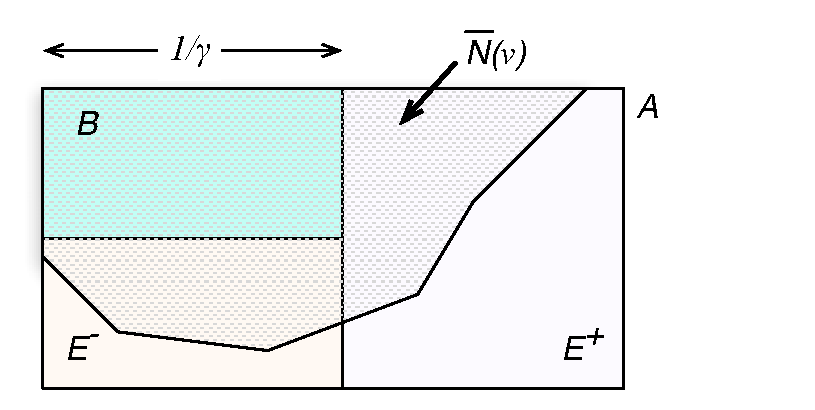
\includegraphics[width=3.2in]{proof_of_lemma_PD'3a.pdf}
\caption{Illustration of the sets $\wbarN(\nu)$, $A$, $B$,
  $E^-$ and $E^+$ in the proof of Lemma~\ref{lem: PD1:
    primary overlap}. Let $X \Subset Y$ mean that the facility
	sets $X$ is obtained from $Y$ by splitting facilities.
	We then have $A \Subset \wtildeN(j)$, 
	$B \Subset  \wtildeclsnb(j) \cap \wbarclsnb(\kappa)$, 
	$E^- \Subset  \wtildeclsnb(j) - \wbarclsnb(\kappa)$, 
	$E^+ \Subset \wtildeN(j) - \wtildeclsnb(j)$.}
\label{fig: sets lemma PD'3a}
\end{center}
\end{figure}

  We define the sets $A$, $B$, $E^-$ and $E^+$ as the subsets of
  $\facilityset$ (the final set of facilities) that were obtained from
  splitting facilities in the sets $\wtildeN(j)$, $\wtildeclsnb(j)\cap
  \wbarclsnb(\kappa)$, $\wtildeclsnb(j) - \wbarclsnb(\kappa)$ and
  $\wtildeN(j) - \wtildeclsnb(j)$, respectively.  (See
  Figure~\ref{fig: sets lemma PD'3a}.)  We claim that at the end
  $B\subseteq \wbarclsnb(\nu)$, with the caveat that the ties in the
  definition of $\wbarclsnb(\nu)$ are broken in favor of the
  facilities in $B$.  (This is the tie-breaking rule that we mentioned
  in the definition of $\wbarclsnb(\nu)$.)  This will be sufficient to
  prove the lemma because $B\neq\emptyset$, by the algorithm.

  We now prove this claim. In this paragraph $\wbarN(\nu)$ denotes the
  final set $\wbarN(\nu)$ after both phases are completed. Thus the total
connection value of $\wbarN(\nu)$ to $\nu$ is $1$.
	Note first that
  $B\subseteq \wbarN(\nu) \subseteq A$, because we never remove
  facilities from $\wbarN(\nu)$ and we only add facilities from
  $\wtildeN(j)$.  Also, $B\cup E^-$ represents the facilities obtained
  from $\wtildeclsnb(j)$, so $\sum_{\mu\in B\cup E^-} \bary_{\mu} =
  1/\gamma$.  This and $B\subseteq \wbarN(\nu)$ implies that the total
  connection value of $B\cup (\wbarN(\nu)\cap E^-)$ to $\nu$ is at
  most $1/\gamma$. But all facilities in $B\cup (\wbarN(\nu)\cap E^-)$
  are closer to $\nu$ (taking into account our tie breaking in property (NB))
 	than those in $E^+\cap \wbarN(\nu)$. It follows
  that $B\subseteq \wbarclsnb(\nu)$, completing the proof.
\end{proof}

%%%%%%%%%%%%%%

\begin{lemma}\label{lem: PD1: primary optimal}
  Property (PD'.\ref{PD:assign:cost}) holds.
\end{lemma}

\begin{proof}
This proof is similar to that for Lemma~\ref{lem: PD:assign:cost holds}.
For a client $j$ and demand $\eta$, we will write
$\tcccls^\eta(j)$ and $\dmaxcls^\eta(j)$ to denote the values of
$\tcccls(j)$ and $\dmaxcls(j)$ at the time when $\eta$
was created. (Here $\eta$ may or may not be a demand of client $j$).

Suppose $\nu \in j$ is assigned to a primary demand $\kappa \in p$.
By the way primary demands are constructed in the partitioning
algorithm, $\wtildeclsnb(p)$ becomes $\wbarN(\kappa)$, which is equal
to the final value of $\wbarclsnb(\kappa)$. So we have
$\clsdist(\kappa) = \tcccls^\kappa (p)$ and $\clsmax(\kappa) =
\dmaxcls^\kappa(p)$. Further, since we choose $p$ to minimize
$\tcccls(p) + \dmaxcls(p)$, we have that $\tcccls^\kappa(p) +
\dmaxcls^\kappa(p) \leq \tcccls^\kappa(j) + \dmaxcls^\kappa(j)$.

Using an argument analogous to that in the proof of Lemma~\ref{lem: tcc optimal}, 
our modified partitioning algorithm guarantees that
  $\tcccls^{\kappa}(j) \leq \tcccls^{\nu}(j) \leq \clsdist(\nu)$ and
  $\dmaxcls^{\kappa}(j) \leq \dmaxcls^{\nu}(j) \leq \clsmax(\nu)$ since $\nu$ was
  created later.
  Therefore, we have
%
  \begin{align*}
    \clsdist(\kappa) + \clsmax(\kappa) &= \tcccls^{\kappa}(p) +	\dmaxcls^{\kappa}(p) 
					\\
					&\leq \tcccls^{\kappa}(j) + \dmaxcls^{\kappa}(j) 
					\leq \tcccls^{\nu}(j) + \dmaxcls^{\nu}(j) 
					\leq \clsdist(\nu) + \clsmax(\nu),
  \end{align*}
%
completing the proof.
\end{proof}

%%%%%%%%

Now we have completed the proof that the computed partitioning satisfies
all the required properties. 


\paragraph{Algorithm~{\EBGS}.}
The complete algorithm starts with solving the LP(\ref{eqn:fac_primal}) and
computing the partitioning described earlier in this section.  Given
the partitioned fractional solution $(\barbfx, \barbfy)$ with the
desired properties, we start the process of opening facilities and
making connections to obtain an integral solution. To this end, for
each primary demand $\kappa\in P$, we open exactly one facility
$\phi(\kappa)$ in $\wbarclsnb(\kappa)$, where each
$\mu\in\wbarclsnb(\kappa)$ is chosen as $\phi(\kappa)$ with
probability $\gamma\bary_{\mu}$. For all facilities
$\mu\in\facilityset - \bigcup_{\kappa\in P}\wbarclsnb(\kappa)$, we
open them independently, each with probability
$\gamma\bary_{\mu}$. 

We claim that all probabilities are well-defined, that is
$\gamma\bary_{\mu} \le 1$ for all $\mu$. Indeed, if $\bary_{\mu}>0$ then
$\bary_{\mu} = \barx_{\mu\nu}$ for some $\nu$, by Property~(CO).
If $\mu\in \wbarclsnb(\nu)$ then the definition of close
neighborhoods implies that $\barx_{\mu\nu} \le 1/\gamma$.
If $\mu\in \wbarfarnb(\nu)$ then
$\barx_{\mu\nu} \le 1-1/\gamma \le 1/\gamma$, because $\gamma < 2$.
Thus $\gamma\bary_{\mu} \le 1$, as claimed.

Next, we connect demands to facilities.  Each primary demand
$\kappa\in P$ will connect to the only open facility $\phi(\kappa)$ in
$\wbarclsnb(\kappa)$.  For each non-primary demand $\nu\in \demandset
- P$, if there is an open facility in $\wbarclsnb(\nu)$ then we
connect $\nu$ to the nearest such facility. Otherwise, we connect
$\nu$ to the nearest far facility in $\wbarfarnb(\nu)$ if one is
open. Otherwise, we connect $\nu$ to its \emph{target facility}
$\phi(\kappa)$, where $\kappa$ is the primary demand that $\nu$ is
assigned to.

%%%%%%%%%%%

\paragraph{Analysis.}
By the algorithm, for each client $j$, all its $r_j$ demands are connected to
open facilities. If two different siblings $\nu,\nu'\in j$ are assigned, respectively,
to primary demands $\kappa$, $\kappa'$ then, by
Properties~(SI'.\ref{SI1:siblings disjoint}), (SI'.\ref{SI1:primary
  disjoint}), and (PD'.\ref{PD1:disjoint}) we have
%
\begin{equation*}
( \wbarN(\nu) \cup \wbarclsnb(\kappa)) \cap (\wbarN(\nu')\cup \wbarclsnb(\kappa')) = \emptyset.
\end{equation*}
%
This condition guarantees that $\nu$ and $\nu'$ are assigned to different facilities,
regardless whether they are connected to a neighbor facility or to its target facility.
Therefore the computed solution is feasible.

\medskip

We now estimate the cost of the solution computed by Algorithm {\EBGS}. The lemma
below bounds the expected facility cost.

%%%%%%%%%%

\begin{lemma} \label{lem: EBGS facility cost}
The expectation of facility cost $F_{\smallEBGS}$ of Algorithm~{\EBGS} is at most $\gamma F^\ast$.
\end{lemma}

\begin{proof}
By the algorithm, each facility $\mu\in \facilityset$ is opened with
probability $\gamma \bary_{\mu}$, independently of whether it belongs to the
close neighborhood of a primary demand or not. Therefore, by
  linearity of expectation, we have that the expected facility cost is
%
\begin{equation*}
	\Exp[F_{\smallEBGS}] = \sum_{\mu \in \facilityset} f_\mu \gamma \bary_{\mu} 
			= \gamma \sum_{i\in \sitesset} f_i \sum_{\mu\in i} \bary_{\mu} 
			= \gamma \sum_{i \in \sitesset} f_i y_i^\ast = \gamma F^\ast,
\end{equation*}
%
where the third equality follows from (PS.\ref{PS:yi}).
\end{proof}

%%%%%%%%%%%

\medskip

In the remainder of this section we focus on the connection cost. Let $C_{\nu}$ be the
random variable representing the connection cost of a demand $\nu$. Our objective is
to show that the expectation of $\nu$ satisfies
%
\begin{equation}
\Exp[C_\nu]	\leq \concost(\nu) \cdot \max\left\{\frac{1/e+1/e^\gamma}{1-1/\gamma}, 1 + \frac{2}{e^\gamma}\right\}.
		\label{eqn: expectation of C_nu for EBGS}
\end{equation}
%
If $\nu$ is a primary demand then, due to the algorithm, we have $\Exp[C_{\nu}] =
\clsdist(\nu) \le \concost(\nu)$, so (\ref{eqn: expectation of C_nu for EBGS}) is
easily satisfied.

Thus for the rest of the argument we will focus on the case when $\nu$
is a non-primary demand.  Recall that the
algorithm connects $\nu$ to the nearest open facility in
$\wbarclsnb(\nu)$ if at least one facility in $\wbarclsnb(\nu)$ is
open. Otherwise the algorithm connects $\nu$ to the nearest open
facility in $\wbarfarnb(\nu)$, if any. In the event that no facility in
$\wbarN(\nu)$ opens, the algorithm will connect $\nu$ to its target
facility $\phi(\kappa)$, where $\kappa$ is the primary demand that
$\nu$ was assigned to, and $\phi(\kappa)$ is the only facility open in
$\wbarclsnb(\kappa)$. Let $\Lambda^\nu$ denote the event that at least
one facility in $\wbarN(\nu)$ is open and $\Lambda^\nu_{\cls}$ be the
event that at least one facility in $\wbarclsnb(\nu)$ is open.
$\neg \Lambda^\nu$ denotes the complement event of $\Lambda^\nu$, that is,
the event that none of $\nu$'s neighbors opens. 
We want to estimate the following three conditional expectations: 
%
\begin{equation*}
  \Exp[C_{\nu} \mid
  \Lambda^\nu_{\cls}],\quad \Exp[C_{\nu} \mid \Lambda^\nu \wedge \neg
  \Lambda^\nu_{\cls}], \quad\text{and}\quad \Exp[C_{\nu} \mid \neg \Lambda^\nu], 
\end{equation*}
%
and their associated probabilities.

We start with a lemma dealing with the third expectation,
$\Exp[C_\nu\mid\neg \Lambda^{\nu}] = \Exp[d_{\phi(\kappa)\nu} \mid
\Lambda^{\nu}]$. The proof of this lemma relies on
Properties~(PD'.\ref{PD1:assign:overlap}) and
(PD'.\ref{PD1:assign:cost}) of modified partitioning and follows the
reasoning in the proof of a similar lemma
in~\cite{ByrkaGS10,ByrkaA10}.

%%%%%%%

\begin{lemma}\label{lem: EBGS target connection cost}
Assuming that no facility in $\wbarN(\nu)$ opens, the expected connection
cost of $\nu$ is
%
\begin{equation}
  \Exp[C_{\nu} \mid \neg \Lambda^{\nu}] \leq
  \clsdist(\nu) + 2\fardist(\nu).
  \label{eqn: expected connection cost target facility}
\end{equation}
%
\end{lemma}

\begin{proof}
It suffices to show a stronger inequality
\begin{equation}
  \Exp[C_{\nu} \mid \neg \Lambda^{\nu}] \leq
  \clsdist(\nu) + \clsmax(\nu) + \fardist(\nu)
			\label{eqn: lemma ebgs indirect connection cost},
\end{equation}
which then implies (\ref{eqn: expected connection cost
  target facility}) because $\clsmax(\nu) \leq
\fardist(\nu)$.  The proof of (\ref{eqn: lemma ebgs indirect
  connection cost}) is similar to that in
\cite{ByrkaA10}. For the sake of completeness, we provide it
here, formulated in our terminology and notation.

Assume that the event $\neg \Lambda^{\nu}$ is true, that is Algorithm~{\EBGS}
does not open any facility in $\wbarN(\nu)$.
Let $\kappa$ be the primary demand that $\nu$ was assigned to. Also let
%K
\begin{equation*}
K = \wbarclsnb(\kappa) \setminus \wbarN(\nu), \quad
V_{\cls} = \wbarclsnb(\kappa) \cap \wbarclsnb(\nu) \quad \textrm{and}\quad 
V_{\far} = \wbarclsnb(\kappa) \cap \wbarfarnb(\nu).
\end{equation*}
% 
Then $K, V_{\cls}, V_{\far}$ form a partition of
$\wbarclsnb(\kappa)$, that is, they are disjoint and their union is $\wbarclsnb(\kappa)$.
Moreover, we have that $K$ is not empty, because Algorithm~{\EBGS}
opens some facility in $\wbarclsnb(\kappa)$ and this facility cannot be in $V_{\cls}\cup V_{\far}$,
by our assumption. 
We also have that $V_{\cls}$ is not empty due to (PD'.\ref{PD1:assign:overlap}). 

Recall that $D(A,\eta) = \sum_{\mu\in A}d_{\mu\eta}\bary_{\mu}/\sum_{\mu\in A}\bary_{\mu}$
is the average distance between a demand $\eta$ and the facilities in a set $A$. We shall show that
%
\begin{equation}
	 D(K, \nu) \leq \clsdist(\kappa)+\clsmax(\kappa) + \fardist(\nu).
				\label{eqn: bound on D(K,nu)}
\end{equation}
%
This is sufficient, because, by the algorithm, $D(K,\nu)$ is exactly 
the expected connection cost for demand $\nu$ conditioned on
the event that none of $\nu$'s neighbors 
opens, that is the left-hand side of (\ref{eqn: lemma ebgs indirect connection cost}).
Further, (PD'.\ref{PD1:assign:cost}) states that 
$\clsdist(\kappa)+\clsmax(\kappa) \le \clsdist(\nu) + \clsmax(\nu)$, and thus
(\ref{eqn: bound on D(K,nu)})  implies (\ref{eqn: lemma ebgs indirect connection cost}).

\medskip

The proof of (\ref{eqn: bound on D(K,nu)}) is by analysis of several cases.
%

\medskip
\noindent
{\mycase{1}} $D(K, \kappa) \leq \clsdist(\kappa)$. For any
facility $\mu \in V_{\cls}$ (recall that $V_{\cls}\neq\emptyset$), 
we have $d_{\mu\kappa} \leq \clsmax(\kappa)$ 
and $d_{\mu\nu} \leq \clsmax(\nu) \leq \fardist(\nu)$. Therefore, using the
case assumption, we get
	$D(K,\nu) \leq D(K,\kappa) + d_{\mu\kappa} + d_{\mu\nu} 
				\leq \clsdist(\kappa) + \clsmax(\kappa) + \fardist(\nu)$.

\medskip
\noindent
{\mycase{2}} There exists a facility $\mu\in V_{\cls}$ such that
  $d_{\mu\kappa} \leq \clsdist(\kappa)$. Since $\mu\in V_{\cls}$, we infer
  that $d_{\mu\nu} \leq \clsmax(\nu) \leq \fardist(\nu)$.  Using
  $\clsmax(\kappa)$ to bound $D(K, \kappa)$, we have $D(K, \nu)
  \leq D(K, \kappa) + d_{\mu\kappa} + d_{\mu\nu} \leq
  \clsmax(\kappa) + \clsdist(\kappa) + \fardist(\nu)$.

\medskip
\noindent
{\mycase{3}} In this case we assume that neither of Cases~1 and 2 applies, that is
 $D(K, \kappa) > \clsdist(\kappa)$ and every $\mu \in V_{\cls}$ satisfies
 $d_{\mu\kappa} >  \clsdist(\kappa)$. This implies that
$D(K\cup V_{\cls}, \kappa) > \clsdist(\kappa) = D(\wbarclsnb(\kappa), \kappa)$.
Since sets $K$, $V_{\cls}$ and $V_{\far}$ form a partition of $\wbarclsnb(\kappa)$,
we obtain that in this case $V_{\far}$ is not
empty and $D(V_{\far}, \kappa) < \clsdist(\kappa)$. 
Let $\delta = \clsdist(\kappa) - D(V_{\far}, \kappa) > 0$. 
We now have two sub-cases:
%
\begin{description}
	
\item{\mycase{3.1}} {$D(V_{\far}, \nu) \leq \fardist(\nu) + \delta$}.
  Substituting $\delta$, this implies that $D(V_{\far}, \nu) +
  D(V_{\far},\kappa) \le \clsdist(\kappa) + \fardist(\nu)$.  From the
  definition of the average distance $D(V_{\far},\kappa)$ and
  $D(V_{\far}, \nu)$, we obtain that there exists some $\mu \in
  V_{\far}$ such that $d_{\mu\kappa} + d_{\mu\nu} \leq
  \clsdist(\kappa) + \fardist(\nu)$.  Thus $D(K, \nu) \leq D(K,
  \kappa) + d_{\mu\kappa} + d_{\mu\nu} \leq \clsmax(\kappa) +
  \clsdist(\kappa) + \fardist(\nu)$.

\item{\mycase{3.2}} {$D(V_{\far}, \nu) > \fardist(\nu) + \delta$}.
  The case assumption implies that $V_{\far}$ is a proper subset of
  $\wbarfarnb(\nu)$, that is $\wbarfarnb(\nu) \setminus V_{\far}
  \neq\emptyset$.  Let $\hat{y} = \gamma \sum_{\mu\in V_{\smallfar}}
  \bary_{\mu}$.  We can express $\fardist(\nu)$ using $\hat{y}$ as
  follows
%
\begin{equation*}
\fardist(\nu) = D(V_{\far},\nu) \frac{\hat{y}}{\gamma-1} +
    D(\wbarfarnb(\nu)\setminus V_{\far}, \nu) \frac{\gamma-1-\hat{y}}{\gamma-1}.
\end{equation*}
%
Then, using the case condition and simple algebra, we have
%
  \begin{align}
    \clsmax(\nu) &\leq D(\wbarfarnb(\nu) \setminus V_{\far}, \nu) 
			\notag
		\\
		&\leq \fardist(\nu) - \frac{\hat{y}\delta}{\gamma-1-\hat{y}} 
		\leq \fardist(\nu) - \frac{\hat{y}\delta}{1-\hat{y}},
			\label{eqn: case 3, bound on C_cls^max(nu)}
  \end{align}
%
where the last step follows from $1 < \gamma < 2$. 

On the other hand, since $K$, $V_{\cls}$, and $V_{\far}$ form a partition of $\wbarclsnb(\kappa)$,
we have
$\clsdist(\kappa) = (1-\hat{y}) D(K\cup V_{\cls}, \kappa) + \hat{y} D(V_{\far}, \kappa)$.
Then using the definition of $\delta$ we obtain
%
\begin{equation}
    D(K \cup V_{\cls}, \kappa) = \clsdist(\kappa) + \frac{\hat{y}\delta}{1-\hat{y}}.
				\label{eqn: formula for D(V_cls,kappa)}
\end{equation}
%
  Now we are essentially done. If there exists some $\mu \in V_{\cls}$ such
  that $d_{\mu\kappa} \leq \clsdist(\kappa) +
  \hat{y}\delta/(1-\hat{y})$, then	we have
%
  \begin{align*}
    D(K, \nu) &\leq D(K, \kappa) + d_{\mu\kappa} + d_{\mu\nu} \\
    &\leq \clsmax(\kappa) + \clsdist(\kappa) +
    			\frac{\hat{y}\delta}{1-\hat{y}}
    + \clsmax(\nu)\\
    &\leq \clsmax(\kappa) + \clsdist(\kappa) + \fardist(\nu),
  \end{align*}
%
where we used (\ref{eqn: case 3, bound on C_cls^max(nu)}) in the last step.
  Otherwise, from (\ref{eqn: formula for D(V_cls,kappa)}),
we must have $D(K, \kappa) \leq \clsdist(\kappa) +
  \hat{y}\delta/(1-\hat{y})$. Choosing any $\mu \in V_{\cls}$, it follows that
%
  \begin{align*}
    D(K, \nu) &\leq D(K, \kappa) + d_{\mu\kappa} + d_{\mu\nu} \\
    &\leq \clsdist(\kappa) + \frac{\hat{y}\delta}{1-\hat{y}} +
    		\clsmax(\kappa)  + \clsmax(\nu)\\
    &\leq \clsdist(\kappa) + \clsmax(\kappa) + \fardist(\nu),
  \end{align*}
%
again using (\ref{eqn: case 3, bound on C_cls^max(nu)}) in the last step.

\end{description}

This concludes the proof of (\ref{eqn: expected connection
  cost target facility}).  As explained earlier,
Lemma~\ref{lem: EBGS target connection cost} follows.
\end{proof}

Next, we derive some estimates for the expected cost of direct
connections.  The next technical lemma is a generalization of
Lemma~\ref{lem: echs expected C_nu}. In Lemma~\ref{lem: echs expected
  C_nu} we bound the expected distance to the closest open facility in
$\wbarN(\nu)$, conditioned on at least one facility in $\wbarN(\nu)$
being open. The lemma below provides a similar estimate for an
arbitrary set $A$ of facilities in $\wbarN(\nu)$, conditioned on that
at least one facility in set $A$ is open.  Recall that $D(A,\nu) =
\sum_{\mu \in A} d_{\mu\nu} \bary_{\mu} / \sum_{\mu \in A}
\bary_{\mu}$ is the average distance from $\nu$ to a facility in $A$. 

%%%%%%%

\begin{lemma}\label{lem: expected distance in EBGS}
  For any non-empty set $A\subseteq \wbarN(\nu)$, let $\Lambda^\nu_A$ be
  the event that at least one facility in $A$ is opened by Algorithm
  {\EBGS}, and denote by $C_\nu(A)$ the random variable representing
  the distance from $\nu$ to the closest open facility in $A$.  Then
  the expected distance from $\nu$ to the nearest open facility in
  $A$, conditioned on at least one facility in $A$ being opened, is
%
\begin{equation*}
	\Exp[C_\nu(A) \mid \Lambda^\nu_A ] \le D(A,\nu).
\end{equation*}
\end{lemma}

\begin{proof}
  The proof follows the same reasoning as the proof of Lemma~\ref{lem:
    echs expected C_nu}, so we only sketch it here. We start with a
  similar grouping of facilities in $A$: for each primary demand
  $\kappa$, if $\wbarclsnb(\kappa)\cap A\neq\emptyset$ then
  $\wbarclsnb(\kappa)\cap A$ forms a group. Facilities in $A$ that are
  not in a neighborhood of any primary demand form singleton groups.
  We denote these groups $G_1,...,G_k$. It is clear that the groups
  are disjoint because of (PD'.\ref{PD1:disjoint}). Denoting by
  $\bard_s = D(G_s, \nu)$ the average distance from $\nu$ to a group $G_s$, we
  can assume that these groups are ordered so that $\bard_1\le ... \le
  \bard_k$.

  Each group can have at most one facility open and the events
  representing opening of any two facilities that belong to different
  groups are independent. To estimate the distance from $\nu$ to the
  nearest open facility in $A$, we use an alternative
  random process to make connections, that is easier to
  analyze. Instead of connecting $\nu$ to the nearest open facility in
  $A$, we will choose the smallest $s$ for which $G_s$ has an open
  facility and connect $\nu$ to this facility. (Thus we selected an
  open facility with respect to the minimum $\bard_s$, not the actual
  distance from $\nu$ to this facility.)  This can only increase the
  expected connection cost, thus denoting $g_s = \sum_{\mu\in G_s}
  \gamma\bary_\mu$ for all $s=1,\ldots,k$, and letting $\Prob[\Lambda^\nu_A]$
  be the probability that $A$ has at least one facility open, we have
%
\begin{align}
    \Exp[C_\nu(A) \mid \Lambda^\nu_A] &\leq \frac{1}{\Prob[\Lambda^\nu_A]} (\bard_1 g_1 +
    \bard_2 g_2 (1 - g_1) + \ldots + \bard_k  g_k(1 -
    g_1)\ldots(1-g_{k-1}))
    \label{eqn: dist set to nu 1}
    \\
    &\leq \frac{1}{\Prob[\Lambda^\nu_A]} \frac{\sum_{s=1}^k \bard_s
      g_s}{\sum_{s=1}^k  g_s} (1 - \prod_{s=1}^k (1 -  g_s))
    \label{eqn: dist set to nu 2}
    \\
    \notag
    &= \frac{\sum_{s=1}^k \bard_s g_s}{\sum_{s=1}^k g_s} =
    \frac{\sum_{\mu \in A} d_{\mu\nu} \gamma \bary_{\mu}}{\sum_{\mu
        \in A} \gamma \bary_{\mu}}
    \\
    \notag
    &= \frac{\sum_{s=1}^k d_{\mu\nu} \bary_{\mu}}{\sum_{\mu \in A}
      \bary_{\mu}} = D(A, \nu).
    \\
    \notag
\end{align}
%
Inequality (\ref{eqn: dist set to nu 2}) follows from inequality
(\ref{eq:min expected distance}) in~\ref{sec: ECHSinequality}. The rest of the
derivation follows from $\Prob[\Lambda^\nu_A] = 1 - \prod_{s=1}^k (1 -
g_s)$, and the definition of $\bard_s$, $g_s$ and $D(A,\nu)$.
\end{proof}

A consequence of Lemma~\ref{lem: expected distance in EBGS} is the
following corollary which bounds the other two expectations
of $C_\nu$, when at least one facility is opened in $\wbarclsnb(\nu)$,
and when no facility in $\wbarclsnb(\nu)$ opens but a facility in
$\wbarfarnb(\nu)$ is opened.

%%%%%%%%%

\begin{corollary} \label{coro: EBGS close and far distance} 
%
{\rm (a)} $\Exp[C_{\nu} \mid \Lambda_{\cls}^\nu] \leq \clsdist(\nu)$,
and
{\rm (b)} $\Exp[C_{\nu} \mid \Lambda^\nu \wedge \neg \Lambda_{\cls}^\nu]
    			\leq \fardist(\nu)$.
\end{corollary}

\begin{proof}
When there is an open facility in $\wbarclsnb(\nu)$, the algorithm
  connect $\nu$ to the nearest open facility in
  $\wbarclsnb(\nu)$. When no facility in $\wbarclsnb(\nu)$ opens but
  some facility in $\wbarfarnb(\nu)$ opens, the algorithm connects
  $\nu$ to the nearest open facility in $\wbarfarnb(\nu)$. The rest of
  the proof follows from Lemma~\ref{lem: expected distance in
    EBGS}. By setting the set $A$ in Lemma~\ref{lem: expected distance
    in EBGS} to $\wbarclsnb(\nu)$, we have
%
  \begin{equation*}
    \Exp[C_{\nu} \mid \Lambda_{\cls}^\nu] \leq D(\wbarclsnb(\nu), \nu),
    = \clsdist(\nu),
    \label{eqn: expected connection cost close facility}
  \end{equation*}
% 
proving part (a), and by setting the set $A$ to $\wbarfarnb(\nu)$, we have
%
  \begin{equation*}
    \Exp[C_{\nu}
    \mid \Lambda^\nu \wedge \neg \Lambda_{\cls}^\nu] \leq
    D(\wbarfarnb(\nu), \nu) = \fardist(\nu),
    \label{eqn: expected connection cost far facility}
  \end{equation*}
which proves part (b).
\end{proof}

Given the estimate on the three expected distances when $\nu$ connects
to its close facility in $\wbarclsnb(\nu)$ in (\ref{eqn: expected
  connection cost close facility}), or its far facility in
$\wbarfarnb(\nu)$ in (\ref{eqn: expected connection cost far
  facility}), or its target facility $\phi(\kappa)$ in (\ref{eqn:
  expected connection cost target facility}), the only missing pieces
are estimates on the corresponding probabilities of each event, which
we do in the next lemma. Once done, we shall put all pieces together
and proving the desired inequality on $\Exp[C_{\nu}]$, that is
(\ref{eqn: expectation of C_nu for EBGS}).

The next Lemma bounds the probabilities for events
that no facilities in $\wbarclsnb(\nu)$ and $\wbarN(\nu)$ are
opened by the algorithm.

%%%%%%%%%%%

\begin{lemma}\label{lem: close and far neighbor probability}
{\rm (a)} $\Prob[\neg\Lambda^\nu_{\cls}] \le 1/e$, and
{\rm (b)} $\Prob[\neg\Lambda^\nu] \le 1/e^\gamma$.
\end{lemma}

\begin{proof}
  (a) To estimate $\Prob[\neg\Lambda^\nu_{\cls}]$, we again consider a
  grouping of facilities in $\wbarclsnb(\nu)$, as in the proof of
  Lemma~\ref{lem: expected distance in EBGS}, according to the primary
  demand's close neighborhood that they fall in, with facilities not
  belonging to such neighborhoods forming their own singleton groups.
  As before, the groups are denoted $G_1, \ldots, G_k$. It is easy to
  see that $\sum_{s=1}^k g_s = \sum_{\mu \in \wbarclsnb(\nu)} \gamma
  \bary_{\mu} = 1$. For any group $G_s$, the probability that a
  facility in this group opens is $\sum_{\mu \in G_s} \gamma
  \bary_{\mu} = g_s$ because in the algorithm at most one facility in
  a group can be chosen and each is chosen with probability $\gamma
  \bary_{\mu}$. Therefore the probability that no facility 
  opens is $\prod_{s=1}^k (1 - g_s)$, which is
  at most $e^{-\sum_{s=1}^k g_s} = 1/e$. Therefore we have
  $\Prob[\neg\Lambda^\nu_A] \leq 1/e$.

(b)
  This proof is similar to the proof of (a). The probability $\Prob[\neg\Lambda^\nu]$ is at most
  $e^{-\sum_{s=1}^k g_s} = 1/e^\gamma$, because we now have
  $\sum_{s=1}^k g_s = \gamma \sum_{\mu \in \wbarN(\nu)} \bary_{\mu} =
  \gamma \cdot 1 = \gamma$.
\end{proof}


We are now ready to bound the overall connection cost of
Algorithm~{\EBGS}, namely inequality (\ref{eqn: expectation of C_nu for EBGS}).

%%%%%%%

\begin{lemma}\label{lem: EBGS nu's connection cost}
The expected connection of $\nu$ is
%
\begin{equation*}
\Exp[C_\nu] \le
  \concost(\nu)\cdot\max\Big\{\frac{1/e+1/e^\gamma}{1-1/\gamma}, 1+\frac{2}{e^\gamma}\Big\}.
\end{equation*}
\end{lemma}

\begin{proof}
  Recall that, to connect $\nu$, the algorithm uses the closest facility in
  $\wbarclsnb(\nu)$ if one is opened; otherwise it will try to connect $\nu$
  to the closest facility in $\wbarfarnb(\nu)$. Failing that, it will
  connect $\nu$ to $\phi(\kappa)$, the sole facility open in the
  neighborhood of $\kappa$, the primary demand $\nu$ was assigned
  to. Given that, we estimate $\Exp[C_\nu]$ as follows:
%
  \begin{align}
    \Exp[C_{\nu}] 
		\;&= \;\Exp[C_{\nu}\mid \Lambda^\nu_{\cls}] \cdot \Prob[\Lambda^\nu_{\cls}]	
				\;+\; \Exp[C_{\nu}\mid \Lambda^\nu\ \wedge\neg \Lambda^\nu_{\cls}] 
				\cdot \Prob[\Lambda^\nu\, \wedge\neg \Lambda^\nu_{\cls}]	
				\notag
		\\
		& \quad\quad\quad
				+ \; \Exp[C_{\nu}\mid \neg \Lambda^\nu] \cdot \Prob[\neg \Lambda^\nu]
				\notag
		\\
		&\leq \; \clsdist(\nu) \cdot \Prob[\Lambda^\nu_{\cls}]
			\;+\; \fardist(\nu)	
				\cdot \Prob[\Lambda^\nu\, \wedge\neg \Lambda^\nu_{\cls}]
                      \label{eqn: apply three expected dist}
						\\
                        &\quad\quad\quad
			+\; [\,\clsdist(\nu) + 2\fardist(\nu)\,] \cdot \Prob[\neg\Lambda^\nu]
		\notag
		\\
                &=\; [\,\clsdist(\nu) + \fardist(\nu)\,]\cdot \Prob[\neg\Lambda^\nu] 
						\;+\; 
							[\,\fardist(\nu)   -\clsdist(\nu)\,]
                                \cdot \Prob[\neg\Lambda^\nu_{\cls}]
                              \;+\;  \clsdist(\nu)
                                                        \notag
		\\
             &\leq\; [\,\clsdist(\nu) + \fardist(\nu)\,] \cdot \frac{1}{e^\gamma}
             \;+\; [\,\fardist(\nu) - \clsdist(\nu)\,] \cdot \frac{1}{e}
             \;+\; \clsdist(\nu)
             \label{eqn: probability estimate}
             \\
             \notag
             &=\; \Big(1 - \frac{1}{e} + \frac{1}{e^\gamma}\Big)\cdot \clsdist(\nu)
 				\;+\; \Big(\frac{1}{e} + \frac{1}{e^\gamma}\Big)\cdot\fardist(\nu).
\end{align}
%
Inequality (\ref{eqn: apply three expected dist}) follows from
Corollary~\ref{coro: EBGS close and far distance} and 
Lemma~\ref{lem: EBGS target connection cost}. 
Inequality (\ref{eqn: probability estimate}) follows from 
Lemma~\ref{lem: close and far neighbor probability} and
$\fardist(\nu) - \clsdist(\nu)\ge 0$.

Now define $\rho =\clsdist(\nu)/\concost(\nu)$. It is easy to
see that $\rho$ is between 0 and 1. Continuing the above
derivation, applying (\ref{eqn:avg dist cls dist far dist}), we get
%
\begin{align*}
\Exp[C_{\nu}]
             \;&\le\; \concost(\nu) 
			\cdot\left((1-\rho)\frac{1/e+1/e^\gamma}{1-1/\gamma} 
				+ \rho (1 + \frac{2}{e^\gamma})\right)
			\\
             &\leq \concost(\nu) 
				\cdot \max\left\{\frac{1/e+1/e^\gamma}{1-1/\gamma}, 1 + \frac{2}{e^\gamma}\right\},
\end{align*}
%
and the proof is now complete.
\end{proof}

With Lemma~\ref{lem: EBGS nu's connection cost} proven, we are now ready to bound our total connection cost.
For any client $j$ we have
%
\begin{align*}
\sum_{\nu\in j} C^{\avg}(\nu)
	&= \sum_{\nu\in j}\sum_{\mu\in\facilityset} d_{\mu\nu}\barx_{\mu\nu} 
	\\
	&= \sum_{i\in\sitesset}d_{ij}\sum_{\mu\in i}\sum_{\nu\in j} \barx_{\mu\nu}
	= \sum_{i\in\sitesset} d_{ij}x_{ij}^\ast = C_j^\ast.
\end{align*}
% 
Summing over all clients $j$ we obtain that the total expected connection cost is
%
\begin{equation*}
	\Exp[ C_{\smallEBGS} ] \le  C^\ast\max\left\{\frac{1/e+1/e^\gamma}{1-1/\gamma}, 1+\frac{2}{e^\gamma}\right\}.
\end{equation*}
%
Recall that the expected facility cost is bounded by $\gamma F^\ast$,
as argued earlier. Hence the total expected cost is bounded by $\max\{\gamma,
\frac{1/e+1/e^\gamma}{1-1/\gamma}, 1+\frac{2}{e^\gamma}\}\cdot
\LP^\ast$. Picking $\gamma=1.575$ we obtain the desired ratio.

%%%%%%

\begin{theorem}\label{thm:ebgs}
  Algorithm~{\EBGS} is a $1.575$-approximation algorithm for \FTFP.
\end{theorem}

%% ch5 primal-dual results
\chapter{Primal-dual Algorithms} 
\label{ch: primal-dual} 

In this chapter we present results and discuss combinatorial
algorithms to the FTFP problem. These approaches, although
employ the Linear Program in guiding the algorithm and
deriving approximation ratio, the use of LP is implicit. In
particular, the algorithms do not require solving the LP and
having access to a fractional optimal solution. Two notable
such approaches are primal-dual and dual-fitting. In this
chapter we assume the primal problem is a minimization
problem and the dual problem is a maximization problem, to
be consistent with our {\FTFP} problem. In primal-dual
algorithms, we start with a feasible dual solution, usually
with all dual variables set to zero, then we raise a subset
of dual variables and update the corresponding primal
variables accordingly. At any time, we keep the dual
solution feasible and we stop when the primal solution
becomes feasible. The approximation ratio is derived by a
relaxed version of the complementary slackness conditions.

Another approach, dual-fitting, starts with an empty dual
solution as well, and works in iterations. In each
iteration, the algorithm raises a subset of dual variables,
and updates corresponding primal variables. The algorithm
stops when the primal solution is feasible. The difference
is that in dual-fitting, the dual solution may not be
feasible, and we require the cost of the primal solution
bounded by the value of the possibly infeasible dual
solution. The next step is to find a suitable number
$\gamma$, which may depend on the input size, such that the
dual solution, when divided by $\gamma$, becomes
feasible. It is easy to see that $\gamma$ provides an upper
bound on the approximation ratio, because the value of a
feasible dual solution is a lower bound on the value of an
optimal primal solution.

Jain and Vazirani~\cite{JainV01} designed a primal-dual
algorithm, which we call the JV algorithm, for the {\UFL}
problem. Recall that in the {\UFL}, all demands $r_j =
1$. In the JV algorithm, every client $j$ has a number
$\alpha_j$ associated. All $\alpha_j$ start at zero, and all
clients are unconnected initially. The algorithm has two
phases. The first phase runs in iterations. In each
iteration, all $\alpha_j$ that were not temporarily
connected are raise uniformly. The contribution from a
client $j$ to a facility $i$ is $\max\{0, \alpha_j -
d_{ij}\}$. Whenever a facility received enough total
contribution, that is $\sum_{j\in\clientset} (\alpha_j -
d_{ij})_+ = f_i$, then $i$ is temporarily open and all
clients with $\alpha_j \geq d_{ij}$ temporarily connect to
$i$. The facility $i$ is called the witness of the client
$j$. The first phase concludes when all clients are
temporarily connected. In the second phase, we construct an
auxiliary graph with nodes being temporarily open facilities
in the first phase. Two nodes $i_1$ and $i_2$ are connected
by an edge in this auxiliary graph if there exists some
client $j$ that contributes to both of them, that is,
$\alpha_j > d_{i_1 j}$ and $\alpha_j > d_{i_2 j}$. We then
pick a maximal independent set in the auxiliary graph as the
set of facilities to open. For connections, if a client $j$
has an open facility $i$ with $d_{ij} < \alpha_j$, then it
connects to that facility. Notice that there can be at most
one such facility. If not, and if there exists some open
facility $i$ such that $d_{ij} = \alpha_j$, then $j$
connects to $i$. These two types of connections are called
\emph{direct} connections. If neither is true, then there
exists some temporarily open facility $i$ such that
$\alpha_j \geq d_{ij}$, namely $j$'s witness. Since $i$ is
not open, there must exists some facility $i'$ that is open
and some client $j'$ such that $\alpha_{j'} > d_{i'j}$ and
$\alpha_{j'} > d_{i j'}$. We then connect $j$ to one such
$i'$ and this type of connection is an \emph{indirect}
connection. 

We now analyze the cost of the solution. Due to the
algorithm, we have $\alpha_{j'} \leq \min\{t(i), t(i')\}$
where $t(i)$ is the time that facility $i$ is temporarily
open. The reason is that, if $\alpha_{j'} > t(i)$, then it
would have temporarily connected to facility $i$ earlier so
its $\alpha_{j'}$ value would have been smaller. On the
other hand, since facility $i$ is the witness of client $j$,
we have $t(i) \leq \alpha_j$~\footnote{$t(i) < \alpha_j$ is
  possible if facility $i$ is temporarily open and later $j$
  has $\alpha_j = d_{ij}$ to temporarily connect to facility
  $i$.} Therefore we have $\alpha_j \geq \alpha_{j'} \geq
\max\{d_{i'j'}, d_{i j'}\}$. In addition, we also have
$\alpha_j \geq d_{ij}$. Hence $d_{i'j} \leq d_{i'j'} +
d_{ij'} + d_{ij} \leq \alpha_{j'} + \alpha_{j'} + \alpha_j
\leq 3\alpha_j$. To complete the dual solution, we define
$\beta_{ij} = \alpha_j - d_{ij}$ if facility $i$ is open and
client $j$ contributes to facility $i$, and $\beta_{ij} = 0$
otherwise. Now we estimate the total cost of this dual
solution. For facility cost we have $\sum_{i,j} \beta_{ij}$,
and for connection cost, if a client $j$ is directly
connected, then its $d_{ij} \leq \alpha_j - \beta_{ij}$,
otherwise it is $d_{ij} \leq 3\alpha_j$. The total cost is
hence no more than $3\sum_{j\in\clientset} \alpha_j$. Since
$\{\alpha_j\}$ form a feasible dual solution, we have the
optimal solution value is no less than
$\sum_{j\in\clientset} \alpha_j$. Therefore, we have our
solution costs no more than $3$ times the cost of an optimal
solution.

The fault-tolerant facility location problem ({\FTFL}) was
introduced by Jain and Vazirani~\cite{JainV03} primarily to
demonstrate that their primal-dual algorithm on {\UFL} can
be applied to a more general problem, where clients could
have demand more than $1$, and each facility could be open
or close. A client $j$ with demand $r_j$ needs to be
connected to $r_j$ different facilities. The primal-dual
algorithm by Jain and Vazirani on {\FTFL} gives a ratio of
$3\ln \max_j r_j$. Subsequent attempts on adapting either
the primal-dual approach or the dual-fitting approach to
{\FTFL} with a sub-logarithmic approximation ratio were not
successful, although for the uniform-demand case, that is,
when all $r_j$ are equal, Adrian Bumb~\cite{Bumb02} showed
that the JV algorithm~\cite{JainV01} for {\UFL} can be
adapted to obtain the same ratio $3$ as for {\UFL}. On a
separate paper, Swamy and Shmoys~\cite{SwamyS08} showed that
a greedy algorithm analyzed using dual-fitting can be shown
to have a ratio of $1.52$. For the non-uniform demand case,
the best known result is an $O(\log
n)$-approximation~\cite{JainV03}.

For our problem, {\FTFP}, we have seen in earlier chapters
that it can be approximated with the same ratio as {\UFL}
when LP-rounding is used. However, the attempt to obtain a
sub-logarithmic approximation ratio on {\FTFP} using the
primal-dual algorithm or the dual-fitting algorithm were not
successful. On the positive side, we derive a weak result
that the greedy algorithm does give a $O(\log n)$ ratio for
{\FTFP}. This also sets stage for our presentation of a hard
example in the following section. We remark here that the
$O(\log n)$ ratio does not even use the triangle
inequality. On the negative side, we provide an example
showing that the greedy algorithm with dual-fitting analysis
can at best give a ratio of $O(\log n/ \log\log n)$ under a
very reasonable assumption, which we call the
\emph{local-charging} assumption. As usual we have $n =
|\clientset|$.

In the following we first describe the greedy algorithm and
its analysis. We show that the greedy algorithm is $O(\log
n)$-approximation using the dual-fitting analysis. Then we
present our example showing a lower bound on the
dual-fitting analysis on the greedy algorithm. We conclude
this chapter with some possible approaches to obtain
sub-logarithmic approximation results.

\section{The Greedy algorithm with $O(\log n)$ Ratio}
\label{sec:upp}
In this section we show that the greedy algorithm which
repeatedly picking the best star (the one with minimum
average cost) gives an approximation ratio of $H_n = \ln(n)$
where $n=|\clientset|$ is the number of clients. A star is a
site $i$ and a subset of clients $C'$. The cost of such a
star $S$ is $c(S) = f_i + \sum_{j\in C'} d_{ij}$, and the
average cost of $S$ is $c(S) / |C'|$. Call a client $j$
fully-connected, or \emph{exhausted} if $j$ has made $r_j$
connections. Let $U$ be the set of not fully-connected
clients. While not all clients fully-connected, the
algorithm picks a star $S=(i,C')$ with $C' \subseteq U$, and
open one facility at site $i$. Each client in $C'$ then
makes one more connection with site $i$. The algorithm
terminates when all clients are fully-connected. To see the
algorithm can be implemented to run in polynomial time, one
observes that once a star becomes best, it remains best
until one or more of its member clients become
exhausted. Thus we can accomplish multiple iterations in a
single step and the number of steps is polynomially bounded
by $|\sitesset|\cdot|\clientset|$.

Now we analyze the cost of the solution, using the
dual-fitting analysis similar to Jain
{\etal}~\cite{JainMMSV03}. When we run the greedy algorithm,
for every client $j$, we associate each demand of $j$ with a
number $\alpha_j^l$, which is the average cost of the star
when $l^{th}$ demand of $j$ is connected. Now we let
$\alpha_j = \alpha_j^{r_j}$, that is, take $\alpha_j$ to be
the finishing $\alpha_j^l$, and order clients by increasing
$\alpha_j$. That is,
\begin{equation*}
  \alpha_1 \leq \alpha_2 \leq \ldots \leq \alpha_n
\end{equation*}

Due to the algorithm, for every $j=1,\ldots,n$, we have
\begin{equation*}
  \sum_{l=j}^n (\alpha_j - d_{il})_+ \leq f_i
\end{equation*}
for every site $i$.  The reason is that, when the last
demand of $j$ is connected, all clients $j+1,\ldots,n$ are
still active so (their $\alpha_j$ are still increasing)
their total contribution cannot exceed $f_i$.

Now we take a closer look at the numbers $\{\alpha_j\}$. We
know that the algorithm's total cost is exactly
$\sum_{j=1}^n \sum_{l=1}^{r_j} \alpha_j^l$, which is no more
than $\sum_{j=1}^n r_j \alpha_j$ since we take $\alpha_j$ to
be $\alpha_j^{r_j}$. Now if we can show that $\sum_{j=1}^n
r_j \alpha_j$ is no more than $\gamma \cdot \OPT$, where
$\textrm{OPT}$ is the cost of an integral optimal solution
to the FTFP instance, then we claim our algorithm computes
an integral solution whose cost is within a factor of
$\gamma$ from $\OPT$.

We show that $\sum_{j=1}^n r_j \alpha_j$ is within a factor
of $\gamma$ from $\textrm{OPT}$ by showing that
$\{\alpha_j/\gamma\}$ is a feasible dual solution to the
following program, which is the dual program of the primal
LP for FTFP.
\begin{align*}
  \max\; &\sum_j r_j\alpha_j\\
  \textrm{subject to: }& \sum_{j=1}^n (\alpha_j - d_{ij})_+
  \leq f_i \quad \forall i \in \sitesset\\
\end{align*}

To find the minimum $\gamma$ that would shrink
$\{\alpha_j\}$ to a feasible dual solution, we need to find
a worst case instance to maximize $\gamma$, also it is clear
that the worst case instance must contain a star whose
feasibility requirement would achieves the value of
$\gamma$, and this star would be the worst star in that
instance.

As a first step we can drop the $\max\{0, \cdot\}$, because
we can always find a new star by dropping those $j$ with
$\alpha_j - d_{ij}$ term negative, and that new star would
still be a worst case star. Suppose a worst case star has
$k$ clients, and is with facility $i$, then we have
\begin{equation*}
  \sum_{j=1}^k \alpha_j - d_{ij} \leq f_i
\end{equation*}
Here we rename clients in the new star to be $1,\ldots,k$,
although among them, they are still ordered by their
$\alpha_j$.

Now our goal is to find a supremum of the following program:
\begin{align*}
  \max\; & \frac{\sum_{j=1}^k \alpha_j}{f_i + \sum_{j=1}^k d_{ij}}\\
  \textrm{subject to: } & \sum_{l=j}^k (\alpha_l -
  d_{il})_+\leq f_i \textrm{ for } j=1,\ldots,k\\
\end{align*}
Actually this is a series of programs for $k=1,2,\ldots$.

Since we are dealing with a particular star, we can abstract
away $i$, to obtain the following program:
\begin{align}
  \label{eq:star}
  \max\; & \frac{\sum_{j=1}^k \alpha_j}{f + \sum_{j=1}^k
    d_j}\\ \notag
  \textrm{subject to: } & \sum_{l=j}^k (\alpha_j - d_{l})_+
  \leq f \textrm{ for } j=1,\ldots,k\\ \notag
\end{align}

Now we claim we can drop the $\max\{0, \cdot\}$ operator
because this would relax the constraint in (\ref{eq:star})
and can only make objective value larger (since we are
maximizing), so the real optimal is upper bounded by the
relaxed optimal. This allows us to work on the following
program instead.
\begin{align}
  \label{eq:frlp}
  \max\; & \frac{\sum_{j=1}^k \alpha_j}{f + \sum_{j=1}^k
    d_j}\\ \notag
  \textrm{subject to: } & \sum_{l=j}^k (\alpha_j - d_{l})
  \leq f \textrm{ for } j=1,\ldots,k\\ \notag
\end{align}

For each $j=1,\ldots,k$, the constraint above simply can be
rewritten as
\begin{equation}
  (k-j+1) \alpha_j \leq f + \sum_{l=j}^k d_l \leq f +
  \sum_{l=1}^k d_l.
\end{equation}
The first inequality is a rewrite of the constraint in
(\ref{eq:frlp}) and the second is straightforward.

Therefore we have $\alpha_j \leq (1/(k-j+1)) (f +
\sum_{j=1}^k d_j)$, and it easily follows that
\begin{equation}
  \sum_{j=1}^n \alpha_j \leq (1/k + 1/(k-1) + \ldots + 1) =
  H_k \leq H_n = \ln(n)
\end{equation}
So we have shown that $\{\alpha_j / \gamma\}$ when $\gamma =
H_n$ is a feasible dual solution and therefore
$\sum_{j\in\clientset} r_j \alpha_j$ is no more than
$H_n\cdot \OPT$. As our primal solution has cost no more
than $\sum_{j\in\clientset} r_j \alpha_j$, the greedy
algorithm computes a solution within $H_n$ from the optimal.

The $H_n$ approximation result is rather weak and is hardly
the best approximation ratio possible for the greedy
algorithm. An astute reader might notice that we have not
used the triangle inequality in deriving the approximation
ratio, although we are working on metric {\FTFP}. On the
other hand, similar attemps in adapting the greedy algorithm
for {\UFL} to {\FTFL} and look for a sub-logarithmic ratio
were not successful by other researchers, as described in
the beginning of this chapter. Although {\FTFP} seems to be
easier to approximate than {\FTFL} when LP-rounding
algorithms were used, it seems the fault-tolerant
requirement in both problems sets a hurdle for primal-dual
based techniques. In the following section we provide an
example that illustrates some difficulty when adapting the
dual-fitting analysis to fault-tolerant facility location
problems.

\section{An Example Showing the Difficulty in Obtaining
  $O(1)$ Ratio}

For FTFP, the greedy algorithm that repeatedly picks the
best star until all clients have all demands satisfied can
be implemented in polynomial time. In Section~\ref{sec:upp}
we show that this algorithm is $H_n$-approximation where
$n=|\mathcal C|$ is the number of clients. Since the same
greedy algorithm is shown to have constant approximation
ratio for UFL~\cite{MahdianMSV01}, a natural question to ask
is whether greedy can be shown to have $O(1)$ approximation
ratio. Here we give an example that hints a negative answer.

We assume the greedy algorithm is analyzed using the
dual-fitting technique, which associates with every client
$j$ with a number $\alpha_j$, interpreted as a dual solution
to the LP~(\ref{eqn:fac_dual}). However, the dual solution
$\{\alpha_j\}$ in general may not be feasible. The
dual-fitting technique aims at finding a smallest possible
number $\gamma$ such that, after the dual solution
$\{\alpha_j\}$ is shrinked (divided) by $\gamma$, all dual
constraints are satisfied. That is
\begin{equation*}
\sum_{j\in \mathcal C} (\alpha_j/\gamma
- d_{ij})_+ \leq f_i \qquad \text{ for all } i\in \mathcal F. 
\end{equation*}
That $\gamma$ is taken as the approximation ratio.

In the greedy algorithm, a star with minimum average cost is
picked at each iteration and each member client of that star
then gets one more connection. It is not specified by the
algorithm how we distribute the cost of $f_i$ into member
clients, which is part of the analysis. Nonetheless we
assume that the cost of $f_i$ is distributed among members
only, and not to clients outside this star. We call this
\emph{local charging} assumption. Our second assumption is
that the proposed dual solution $\alpha_j$, is taken as the
average of individual $\alpha_j^l$ for each of the $l^{th}$
demand of client $j$, with $l=1,\ldots,r_j$. That is
$\alpha_j = \sum_{l=1}^{r_j} \alpha_j^l / r_j$. Suppose the
$l^{th}$ demand of $j$ is satisfied while $j$ is in a star
with facility $i$, then $\alpha_j^l = d_{ij} + f_i^{j,l}$,
where $f_i^{j,l}$ is the portion of $f_i$ attributed to $j$
in the analysis. Notice that taking the average implies the
$\alpha_j$ values thus computed make $\sum_{j\in\clientset}
r_j \alpha_j$ equal to the cost of the integral solution by
the greedy algorithm.

%%%%%%%%%%%%%%%%%%% start figure %%%%%%%%%%%%%%%%%%%%%%%%%%%%%
\begin{figure}
  \centering
  \begin{tikzpicture}[auto]
    \node[draw,rectangle,minimum size=.7cm] (fac) at (-4,0) {};
    \node at (-5,0) {$f_1$};
    
    \node[draw,ellipse,minimum width=4cm,minimum
    height=1.8cm] (client1) at
    (6,0) {$n_1 = k^{k-1}, r_1$};
    \node[draw,ellipse,minimum width=4cm,minimum
    height=1.8cm] (client2) at
    (6,-3) {$n_2 = k^{k-2}, r_2$};
    \node[draw,ellipse,minimum width=4cm,minimum
    height=1.8cm] (client3) at
    (6,-6) {$n_3 = k^{k-3}, r_3$};
    \node[draw,ellipse,minimum width=4cm,minimum
    height=1.8cm] (clientk) at
    (6,-12) {$n_k = 1, r_k$};
    
    \node at (-3,-10) {\large{demands $r_1 \ll r_2 \ll \ldots \ll r_k$}};

    \draw (fac) to node {$d_1=0$} (client1);
    \draw[bend right] (fac) to node {$d_2 = d_1 + f_1 /
      n_2$}  (client2);
    \draw[bend right] (fac) to node {$d_3 = d_2 + f_1 /
      n_3$}  (client3);
    \draw[bend right] (fac) to node {$d_k = d_{k-1} + f_1 / n_k$}  (clientk);
  \end{tikzpicture}
  \caption{An example showing the greedy algorithm for FTFP,
    analyzed using dual-fitting, could give a solution with
    cost $\Omega(\log n / \log\log n)$ from the optimal
    value, assuming facility cost can only be charged to
    clients within the star.}
  \label{fig:greedy_lower_bound}
\end{figure}
%%%%%%%%%%%%%%%%% end figure %%%%%%%%%%%%%%%%%%
%%%%%%%%%%%%%%%%%%%%%%%%%%%%%%%%%%%%%%%%%%%%%%%

We now give our example in
Figure~\ref{fig:greedy_lower_bound}. Our example has one
site and $k$ groups of clients. Opening one facility at that
site costs $f_1$. The first group has $n_1$ clients each
with demand $r_1$, all at distance $d_1 = 0$ from $f_1$. The
other groups are listed below:
\begin{align*}
  &d_1 = 0\\
  &d_2 = \frac{f_1}{n_1}\\
  &d_3 = f_1/n_2 + d_2 = f_1/n_2 + f_1/n_1 = f_1 (\frac{1}{n_2} + \frac{1}{n_1})\\
  &\ldots\\
  &d_k = f_1/n_{k-1} + d_{k-1} = f_1 (\frac{1}{n_{k-1}} + \ldots + \frac{1}{n_1})\\
\end{align*}
For the numbers, we need $r_1 \ll r_2 \ll \ldots \ll r_k$,
and $n_1 = u^{k-1}, n_2 = u^{k-2}, \ldots, n_k = u^0 = 1$
for some number $u$ (Actually we take $u=k$, this choice may
not be the best possible).

Call a star with facility cost zero \emph{trivial}. It is
\emph{non-trivial} if the facility has non-zero cost. Now
the greedy execution goes like this: The first non-trivial
star (with $r_1$ replica) is $(f_1, n_1)$. Then we have a
trivial star of zero cost facility and all $n_2$ clients in
group $2$ for $r_1$ replica. The second non-trivial star
(with $r_2$ replica) is $(f_1, n_2)$. Notice that $r_2 \gg
r_1$. The $r_1$ replica of trivial star with group $2$
satisfy $r_1$ demand of the $n_2$ group. After that the
$n_2$ group clients each has residual demand $r_2 - r_1 =
r_2$. The process repeats until the $k^{th}$ group finishes
with $r_k$ new facilities.

According to our local charging assumption, we have
$\alpha_1 = f_1$, now defined as the total dual value of
clients in group $n_1$, regardless how the analysis would
distribute within that group. Similarly $\alpha_2 = f_1 +
n_2 d_2$, and so on. Substituing in the numbers, we have

\begin{align*}
  &\alpha_1 = f_1\\
  &\alpha_2 = f_1 + n_2 d_2 = f_1 + f_1/n_1\cdot n_2 = f_1 (1 + n_2 /
  n_1)\\
  &\alpha_3 = f_1 + n_3 d_3 = f_1 + f_1 (\frac{1}{n_2} +
  \frac{1}{n_1}) n_3 = f_1 (1 + \frac{n_3}{n_2} + \frac{n_3}{n_1})\\
  &\ldots\\
  &\alpha_k = f_1 + n_k d_k = f_1 + f_1 n_k (\frac{1}{n_{k-1}} + \ldots
  \frac{1}{n_1})\\
\end{align*}
Notice that $r_1 \ll r_2 \ll \ldots \ll r_k$ implies $\alpha_j$ is
decided by the max among $\alpha_j^l$.

Now back to the dual constraint, it requires that the shrinking factor
$\gamma$ needs to satisfy the following inequality:
\begin{equation}
  \frac{\alpha_1}{\gamma} - d_1 + \frac{\alpha_2}{\gamma} - d_2 +
  \ldots + \frac{\alpha_k}{\gamma} - d_k \leq f_1.
\end{equation}
Substitute in the $\alpha_j$ values derived above, we have
\begin{align*}
  \gamma &\geq (\sum_{j=1}^k \alpha_j) / (f_1 + \sum_{j=1}^k d_j)\\
  &\geq \frac{f_1 + n_1 d_1 + f_1 + n_2 d_2 + f_1 + n_3 d_3 + \ldots +
    f_1 + n_k
    d_k}{f_1 + n_1 d_1 + n_2 d_2 + \ldots + n_k d_k}\\
  &= 1 + (k-1)f_1 / (f_1 + n_1 d_1 + n_2 d_2 + \ldots + n_k d_k)\\
  &= 1 + (k-1)f_1 / \left(f_1 + n_2 f_1 / n_1 + \ldots + n_k f_1
    (\frac{1}{n_{k-1}} + \frac{1}{n_{k-2}} + \ldots +
    \frac{1}{n_1})\right)\\
  &= 1 + (k-1) / \left(1 + n_2 / n_1 + \ldots + n_k
    (\frac{1}{n_{k-1}} + \frac{1}{n_{k-2}} + \ldots +
    \frac{1}{n_1})\right)\\
  &= 1 + (k-1) / \left(1 + 1/u + \ldots + (\frac{1}{u} + \ldots +
    \frac{1}{u^{k-1}})\right)\\
  &= 1 + (k-1) / \left(1 + k/u + (k-1)/u^2 + \ldots +
    1/u^{k-1}\right)\\
  &\geq 1 + (k-1) / \left(1 + k/u + k/u^2 + \ldots +
    k/u^{k-1}\right)\\
  &= 1 + (k-1) / \left(1 + 1 + 1/k + \ldots + 1/k^{k-2}\right)\\
  &\approx k/2\\
\end{align*}
So for $k$ groups we can force a shrinking factor $\gamma$
as big as $k/2$. Recall that we have greedy being no more
than $H_n$-approximation. Is that a contradiction? No,
because we have the number of clients $n=k^{k-1} + k^{k-1} +
\ldots + 1 = k^k$, so $k = O(\log n / \log\log
n)$. Therefore, the example shows that dual fitting with
local charging cannot hope to get $O(\log n / \log\log n)$
ratio or better.

\paragraph{Remark} Notice this example is similar in spirit
to the $\Omega(\log n/ \log\log n)$ example for Hochbaum's
algorithm for UFL, constructed by Mahdian {\etal}
~\cite{JainMMSV03}.

%% ch6 conclusion
\chapter{Conclusion} \label{ch: conclusion} 

In thisb dissertation we studied the fault-tolerant facility
placement problem ({\FTFP}), a generalization of the
well-known uncapacitated facility location problem
({\UFL}). We demonstrated that the known LP-rounding
algorithms for {\UFL} can be adapted to {\FTFP} while
preserving the approximation ratio. To accomplish this
reduction, we developed two techniques, namely demand
reduction and adaptive partition, which could be of more
general interest. Our results demonstrated that {\FTFP}
seems easier to approximate, compared to {\FTFL}.

We also studied the primal-dual and dual-fitting approach,
and provided a possible explanation on the difficult to
obtain a constant approximation ratio using those techniques.

We hope our work in this dissertation will help other
researchers interested in the fault-tolerant variant of the
facility location problems to develop more insight into the
difficulty and possible solutions when clients demand more
than one facility and we still need to keep total cost under
control.

In anticipating future research, we tend to agree with the
authors, Byrka {\etal}, with their remark on {\UFL} and
{\FTFL}, that both problems are likely to have approximation
algorithms with ratio matching the $1.463$ lower bound. And
from our demand reduction technique, it is almost surely
that {\FTFP} shall have a $1.463$-approximation algorithm,
provided that {\FTFL} can be approximated to meet the lower
bound.

\bibliographystyle{plain}
\bibliography{facility}

\appendix
\chapter{Technical Background}

\section{Linear Programming and Integer Programming}
\label{sec: ILP}

In this section we give a short introduction on Linear
Programming and Integer Programming with an emphasis on
their applicability in design and analysis of approximation
algorithms for {\NP}-optimization problems.

Most {\NP}-optimization problems have a natural integer
program in which we use variables to represent parameters in
the solution that we seek, and write the constraints imposed
by feasiblity of the solution. The objective function is
obtained by the cost function of the solution, specified by
the problem. For example, in the Vertex Cover problem, we
are given a graph $G=(V,E)$ and we are to find a subset $W$
of $V$, such that every edge $e\in E$ has at least one
endpoint in $W$, and we want the set $W$ to have minimum
size. To formulate this problem as an integer program, we
use $x_v \in \{0,1\}$ to denote whether a node $v\in V$ is
in $W$ or not. The constraint is that for every edge
$e=(u,v)$, we have $x_u + x_v \geq 1$. The objective is to
minimize $\sum_{v\in V} x_v$. The integer program for Vertex
Cover is written as
\begin{align*}
  &\text{minimize } \sum_{v\in V} x_v\\
  &\text{subject to } x_u + x_v \geq 1  \qquad \forall (u,v) \in
  E\\
  &x_v \in \{0, 1\} \qquad \forall v \in V\\
\end{align*}
In general an integer program cannot be solved exactly in
polynomial time, as integer programming is
{\NP}-hard. However, if we relax the integral constraint and
allow the variables to take fractional value, we then obtain
a Linear Program (LP) and LP is polynomially solvable, for
example, using the ellipsoid method or the interior point
method. Thus we can first solve the LP optimally, obtaining
a fractional optimal solution to the LP. The value of the
fractional optimal solution is then a lower bound on the
value of the optimal integral solution, assuming a
minimization problem. Our next step is then to round the
fractional solution appropriately, so that we maintain the
feasibility while keeping the cost from increasing too
much. The exact rounding procedure is problem specific and
we shall not delve into the details here. The rounding
relevant to the FTFP problem in this thesis is presented in
detail in Chapter~\ref{ch: lp-rounding}.

We now give a brief introduction of linear programming,
see~\cite{Chvatal83} for an introductory book on this topic.
A general Linear Program can be written as
\begin{align}
  \label{eqn:lp_primal}
  \text{minimize } & \sum_{j=1}^n c_j x_j & \\ \notag
  \text{subject to } & \sum_{j=1}^n a_{ij} x_j \geq b_i,
   & \text{for } i = 1, \ldots, m\\ \notag
   & x_j \geq 0 & \text{for } j = 1, \ldots, n\\ \notag
\end{align}
For the LP above, we can take its dual as
\begin{align}
  \label{eqn:lp_dual}
  \text{maximize } & \sum_{i=1}^m b_i y_i &\\ \notag
  \text{subject to } & \sum_{i=1}^m a_{ij} y_i \leq c_j
   & \text{for } j = 1, \ldots, n\\ \notag
   & y_i \geq 0 & \text{for } i = 1,\ldots,m\\ \notag
\end{align}
The LP (\ref{eqn:lp_primal}) is called the primal program
and the LP (\ref{eqn:lp_dual}) is called the dual program.
The weak duality theorem tells us that, for every feasible
solution $\bfx$ for the primal (\ref{eqn:lp_primal}) and
$\bfy$ for the dual (\ref{eqn:lp_dual}), we have that
$\textbf{c}^T \bfx \geq \textbf{b}^T \bfy$. The strong
duality theorem tells us that if both the primal
(\ref{eqn:lp_primal}) and the dual (\ref{eqn:lp_dual}) are
feasible, then both of them have optimal solution
$\bfx^\ast$ and $\bfy^\ast$ and their objective function
values equal, that is $\textbf{c}^T \bfx^\ast = \textbf{b}^T
\bfy^\ast$. Moreover, the complementary slackness conditions
assert that two feasible solutions $\bfx$ and $\bfy$ are
both optimal to LP (\ref{eqn:lp_primal}) and
(\ref{eqn:lp_dual}) respectively, if and only if, for every
primal variable $x_j$, either $x_j = 0$ or the corresponding
constraint in the dual is tight, that is $\sum_{i=1}^m
a_{ij} y_i = c_j$. And for every dual variable $y_i$, either
$y_i = 0$ or the corresponding constraint in the primal is
tight, that is $\sum_{j=1}^n a_{ij} x_j = b_i$. The
complementary slackness conditions provide a simple way to
validate the optimality when one is presented with two
solutions, proposed to be optimal for the primal and dual
program respectively.

The complementary slackness conditions play a crucial role
in the design and analysis of approximation algorithms. For
example, suppose we have an algorithm that computes a
feasible integral solution $\bfx$ to the primal program
(\ref{eqn:lp_primal}) and a feasible integral solution to
the dual program (\ref{eqn:lp_dual}). Moreover, we know that
the two solutions satisfy a relaxed version of the
complementary slackness conditions: for some numbers
$\gamma$ and $\rho$, we have
\begin{align*}
  \text{either } y_i = 0  \quad \text{or } \quad b_i \leq \sum_{j}
  a_{ij} x_j \leq \gamma\, b_i \qquad \text{for } i = 1,
  \ldots, m.\\
  \text{either } x_j = 0  \quad \text{or } \quad \rho\, c_j \leq
  \sum_{i}a_{ij}y_i \leq c_j \qquad \text{for } j = 1,
  \ldots, n.\\
\end{align*}
Then the integral solution $\bfx$ has cost no more than
$\gamma/\rho$ times the optimal value. In particular, we
have $\sum_{j} c_j x_j \leq \gamma/\rho \sum_{i} b_i y_i$
and the value for a feasible dual solution, namely $\sum_{i}
b_i y_i$, is a lower bound on the optimal value of the
primal program.

As an application of the complementary slackness conditions,
we look at their use in the design and analysis of
algorithms for the facility location problems. Recall that
we define the neighborhood $N(j)$ of a client $j$ as the set
of facilities with $x_{ij}^\ast > 0$, where
$\bfx^\ast,\bfy^\ast$ is some fractional optimal fractional
solution and $\bfalpha^\ast, \bfbeta^\ast$ is some optimal
fractional dual solution. The complementary slackness
conditions provide an upper bound on the maximum distance
from a facility $i \in N(j)$ to a client $j$, since one dual
constraint says $\alpha_j - \beta_{ij} \leq d_{ij}$ and if
the primal solution has $x_{ij}^\ast > 0$, then the
inequality is actually an equality and we have
$\alpha_j^\ast - \beta_{ij}^\ast = d_{ij}$. Together with
$\beta_{ij}^\ast \geq 0$, we have $\alpha_j^\ast \geq
d_{ij}$ for every $i$ such that $x_{ij}^\ast > 0$.

The idea of using relaxed complementary slackness conditions
in designing approximation algorithms for the uncapacitated
facility location problem is demonstrated by Jain and
Vazirani~\cite{JainV01}. They proposed an algorithm that
outputs an integral solution $(\bfx, \bfy)$ to the primal
program (\ref{eqn:fac_primal}) and a feasible (possibly
fractional) solution $(\bfalpha,\bfbeta)$ to the dual
program (\ref{eqn:fac_dual})~\footnote{For the uncapacitated
  facility location problem we have all $r_j = 1$ for
  $j\in\clientset$.}. Moreover, the two solutions satisfy the
conditions that
\begin{align*}
  &\text{either } \sum_{j} \beta_{ij} = f_i  \quad \text{ or
} \quad y_i = 0.\\
  &\text{either } 1/3\, d_{ij} \leq \alpha_j - \beta_{ij}
  \leq d_{ij} \quad \text{ or } \quad x_{ij} = 0.\\
\end{align*}
The solution $(\bfx,\bfy)$ then is an $3$-approximation to
the optimal solution.

\section{Proof of Inequality (\ref{eqn: echs ineq direct
    cost, step 1})}
\label{sec: ECHSinequality}

In Sections~\ref{sec: 1.736-approximation} and \ref{sec:
  1.575-approximation} we use the following inequality
%
\begin{align}
  \label{eq:min expected distance}
  \bard_1 g_1 + \bard_2 g_2 (1-g_1) +
  \ldots &+ \bard_k g_k (1-g_1) (1-g_2) \ldots (1-g_k)\\ \notag
  &\leq \frac{1}{\sum_{s=1}^k g_s} \left(\textstyle\sum_{s=1}^k \bard_s g_s\right)\left(\textstyle\sum_{t=1}^k g_t \textstyle\prod_{z=1}^{t-1} (1-g_z)\right).
\end{align}
%
for $0 < \bard_1\leq \bard_2 \leq \ldots \leq \bard_k$, and
$0 < g_1,...,g_s \le 1$.

\medskip

We give here a new proof of this inequality, much simpler
than the existing proof in \cite{ChudakS04}, and also
simpler than the argument by Sviridenko~\cite{Svi02}.  We
derive this inequality from the following generalized
version of the Chebyshev Sum Inequality:
%
\begin{equation}
  \label{eq:cheby}
  \textstyle{\sum_{i}} p_i \textstyle{\sum_j} p_j a_j b_j \leq \textstyle{\sum_i} p_i a_i \textstyle{\sum_j} p_j b_j,
\end{equation}
%
where each summation runs from $1$ to $l$ and the sequences
$(a_i)$, $(b_i)$ and $(p_i)$ satisfy the following
conditions: $p_i\geq 0, a_i \geq 0, b_i \geq 0$ for all $i$,
$a_1\leq a_2 \leq \ldots \leq a_l$, and $b_1 \geq b_2 \geq
\ldots \geq b_l$.

Given inequality (\ref{eq:cheby}), we can obtain our
inequality (\ref{eq:min expected distance}) by simple
substitution
%
\begin{equation*}
  p_i \leftarrow g_i, a_i \leftarrow \bard_i, b_i \leftarrow
  \Pi_{s=1}^{i-1} (1-g_s),
\end{equation*}
%
for $i = 1,...,k$.

For the sake of completeness, we include the proof of
inequality (\ref{eq:cheby}), due to Hardy, Littlewood and
Polya~\cite{HardyLP88}. The idea is to evaluate the
following sum:
%
\begin{align*}
  S &= \textstyle{\sum_i} p_i \textstyle{\sum_j} p_j a_j b_j - \textstyle{\sum_i} p_i a_i \textstyle{\sum_j} p_j b_j
	\\
  & = \textstyle{\sum_i \sum_j} p_i p_j a_j b_j - \textstyle{\sum_i \sum_j} p_i a_i p_j b_j
	\\
  & = \textstyle{\sum_j \sum_i} p_j p_i a_i b_i - \textstyle{\sum_j \sum _i} p_j a_j p_i b_i
	\\
	&= \half \cdot \textstyle{\sum_i \sum_j} (p_i p_j a_j b_j - p_i a_i p_j b_j + p_j p_i a_i
  							b_i - p_j a_j p_i b_i)
\\
  &= \half \cdot \textstyle{\sum_i \sum_j} p_i p_j (a_i - a_j)(b_i - b_j) \leq 0.
\end{align*}
The last inequality holds because $(a_i-a_j)(b_i-b_j) \leq
0$, since the sequences $(a_i)$ and $(b_i)$ are ordered
oppositely.


\end{document}

% marek Tue Jul  3 10:21:05 PDT 2012
% marek Sun Jul  1 14:57:39 PDT 2012
% lyan Sat Jun 30 2012, 22:01:27
% marek Sat Jun 30 10:08:59 PDT 2012
% lyan Fri Jun 29 19:54:18 PDT 2012
% marek Thu Jun 28 09:21:14 PDT 2012
% lyan Thu Jun 28 00:11:28 PDT 2012
% marek Wed Jun 27 11:24:07 PDT 2012
% lyan Wed Jun 27 2012, 10:08:21
% marek Tue Jun 26 14:48:45 PDT 2012
% lyan Mon Jun 25 2012, 22:23:13
% marek Sun Jun 24 16:46:23 PDT 2012
% marek Wed Jun 20 04:42:40 PDT 2012
% lyan, Sun Jun 17 2012, 09:49:22
% marek Sat Apr  7 16:42:21 PDT 2012
% marek Thu Apr  5 11:39:58 PDT 2012
% marek Wed Apr  4 11:28:20 PDT 2012
% lyan, 04/01/12 10:20 PM
% lyan, Mon Mar 26 2012, 09:10:54
% lyan, Tue Mar 20 2012, 23:28:17
% lyan, 03/18/12 12:28 PM
% marek Sat Mar 17 13:42:32 PDT 2012
% marek, Wed Mar  7 21:28:24 PST 2012
% marek Mon Mar 12 12:08:25 PDT 2012



\end{document}

%% reference
%% http://www.maths.qmul.ac.uk/~fv/books/mw/mwbook.pdf
%%
%% TODO: pdflatex has font issue with \beta k, ligature?

%% 05/15/2013, first draft